\chapter{Μεθοδολογία}
\label{ch:chapter3}

Στο παρόν κεφαλαίο αυτό παρουσιάζεται η μεθοδολογία που ακολουθήθηκε
κατά την διάρκεια της σύλλογης των δεδομένων των πειραμάτων με το
\textlatin{GitHub Copilot} και με το \textlatin{GitHub Copilot Chat}.
Αρχικά, η επιλογή της εφαρμογής πάνω στην οποία το \textlatin{GitHub
Copilot} αξιολογήθηκε, περιγράφεται παρακάτω.

\section{Επιλογή Εφαρμογής}

Για την επιλογή της κατάλληλης εφαρμογής, λήφθηκαν οι παρακάτω
παράμετροι υπ' όψιν:

\begin{itemize}
  \item
    \textbf{Πολυπλοκότητα της εφαρμογής:} Η εφαρμογή πρέπει να είναι
    αρκετά πολύπλοκη ώστε να απαιτεί την χρήση του \textlatin{GitHub
    Copilot} για την ανάπτυξη του κώδικα.
  \item
    \textbf{Τύπος της εφαρμογής:} Η εφαρμογή πρέπει να είναι μια ιδέα
    αντίστοιχη με τις υπόλoιπες υλοποιήσεις του κλάδου της Μηχανικής
    Λογισμικού και συγκεκριμένα της Ανάπτυξης Ιστότοπων
    \textlatin{\textbf{Web Development}}.
  \item
    \textbf{Γλώσσα της εφαρμογής και Τεχνολογική Στοίβα
    (\textlatin{Technology Stack}):} Η επιλογή της Τεχνολογικής Στοίβας
    πρέπει να γίνει με βάση μοντέρνες τεχνολογίες και με ευρεία χρήση,
    προκειμένου το μοντέλο να έχει την περισσότερη εμπειρία και τις
    καλύτερες αποδόσεις, αλλά και να γίνεται μια αξιολόγηση με πραγματικά
    και εξελισσόμενα εργαλεία.
\end{itemize}

Με βάση τις παραπάνω παραμέτρους, επιλέχθηκε η ανάπτυξη μιας εφαρμογής η
οποία θα αποτελείται από έναν ιστότοπο που θα παρέχει ένα μέσο δικτύωσης
που αφορά τα βιντεοπαιχνίδια. Η εφαρμογή αυτή είχε ήδη αναπτυχθεί στα
πλαίσια του μαθήματος ``Μηχανική Λογισμικού Ι'', επομένως οι βασικές
ανάγκες και λειτουργίες της εφαρμογής είχαν καταγραφθεί. Η επιλογή αυτή
έγινε προκειμένου η αξιολόγηση του κώδικα και των προτάσεων του
\textlatin{GitHub Copilot} να μην έχει αλλαγές με βάση τις αλλαγές που
προέκυψαν κατά τον σχεδιασμό της εφαρμογής. Η εφαρμογή αποτελείται από
τρεις (3) βασικές λειτουργίες:

\begin{itemize}
  \item
    Κριτική παιχνιδιών και κοινοποίηση των κριτικών των χρηστών με τους
    υπόλοιπους χρήστες της εφαρμογής.
  \item
    Διαχείριση και κοινοποίηση λιστών \textlatin{(playlists)} από
    βιντεοπαιχνίδια με τους υπόλοιπους χρήστες της εφαρμογής.
  \item
    Δυνατότητα στον χρήστη να σχολιάσει τις κριτικές των άλλων χρηστών,
    καθώς και να ``ακολουθήσει'' άλλους χρήστες, λαμβάνοντας ειδοποιήσεις
    για τις ενέργειές τους.
\end{itemize}

Παρατίθεται το Σχεσιακό Διάγραμμα Οντοτήτων της εφαρμογής:

\begin{figure}[htbp]
  \centering
  \includegraphics[width=\textwidth]{Relational Database Diagram -
  Component Kit (Community).pdf}
  \caption{Σχεσιακό Διάγραμμα Οντοτήτων της εφαρμογής}
  \label{fig:rdd}
\end{figure}

\subsection{Τεχνολογική Στοίβα \textlatin{Technology Stack}}

Η επιλογή της Τεχνολογικής Στοίβας έγινε με βάση την ευρεία χρήση των
τεχνολογιών αυτών, την ευκολία στην ανάπτυξη και την ευκολία στην
ενσωμάτωση του \textlatin{GitHub Copilot}. Η εφαρμογή αναπτύχθηκε με την
χρήση των παρακάτω τεχνολογιών:

\begin{itemize}
  \item
    \textbf{Γλώσσα Προγραμματισμού}: Η εφαρμογή αναπτύχθηκε με την χρήση
    της γλώσσας προγραμματισμού \textlatin{Typescript} \cite{typescript},
    ενός συντακτικού υπερσυνόλου της γλώσσας \textlatin{JavaScript}
    \cite{javascript}, μια από τις πιο διαδομένες γλώσσες προγραμματισμού
    στον κόσμο. \cite{tiobe, languagechart} Συγκεκριμένα, το 2024 η
    \textlatin{Javascript} ήταν η πρώτη στην λίστα της επισκόπησης του
    \textlatin{Stack Overflow}, μετά από 60.171 ψήφους. \cite{so2024} Την
    πρώτη θέση επίσης έλαβε το 2023 και το 2022. \cite{so2022,so2023}

    Η γλώσσα \textlatin{Javascript} επίσης, είναι η γλώσσα προγραμματισμού
    που εκτελείται στις ιστοσελίδες του διαδικτύου, μέσω της μηχανής
    \textlatin{V8} της \textlatin{Google} \cite{v8} για τους περιηγητές
    διαδικτύου που βασίζονται στην μηχανή περιηγητή ανοιχτού κώδικα
    \textlatin{Chromium} \cite{chromium}, της μηχανής
    \textlatin{SpiderMonkey} της \textlatin{Mozilla} \cite{spidermonkey}
    για τους περιηγητές που χρησιμοποιούν τη μηχανή περιηγητή ανοιχτού
    κώδικα \textlatin{Gecko} \cite{gecko}, και της μηχανής
    \textlatin{JavaScriptCore} της \textlatin{Apple} \cite{javascriptcore}
    για τους περιηγητές που χρησιμοποιούν τη μηχανή περιηγητή
    \textlatin{WebKit} \cite{webkit}, δίνοντάς της τον τίτλο της γλώσσας
    του διαδικτύου.
  \item
    \textbf{Πίσω Ανάπτυξη (\textlatin{Backend Development}):} Η πίσω
    ανάπτυξη της εφαρμογής έγινε με την χρήση της βιβλιοθήκης
    \textlatin{tRPC} \cite{trpc}, μιας βιβλιοθήκης που παρέχει την
    δυνατότητα δημιουργίας \textlatin{API} με την χρήση της γλώσσας
    \textlatin{Typescript} και του περιβάλλοντος εκτέλεσης
    (\textlatin{runtime}) \textlatin{Node.js} \cite{node}. Το
    \textlatin{Node.js} βρισκόταν στην πρώτη θέση για πλαίσιο διαδικτύου
    (\textlatin{web framework}) στην επισκόπηση του \textlatin{Stack
    Overflow} το 2024 \cite{so2024}.
    \begin{figure}[H]
      \begin{center}
        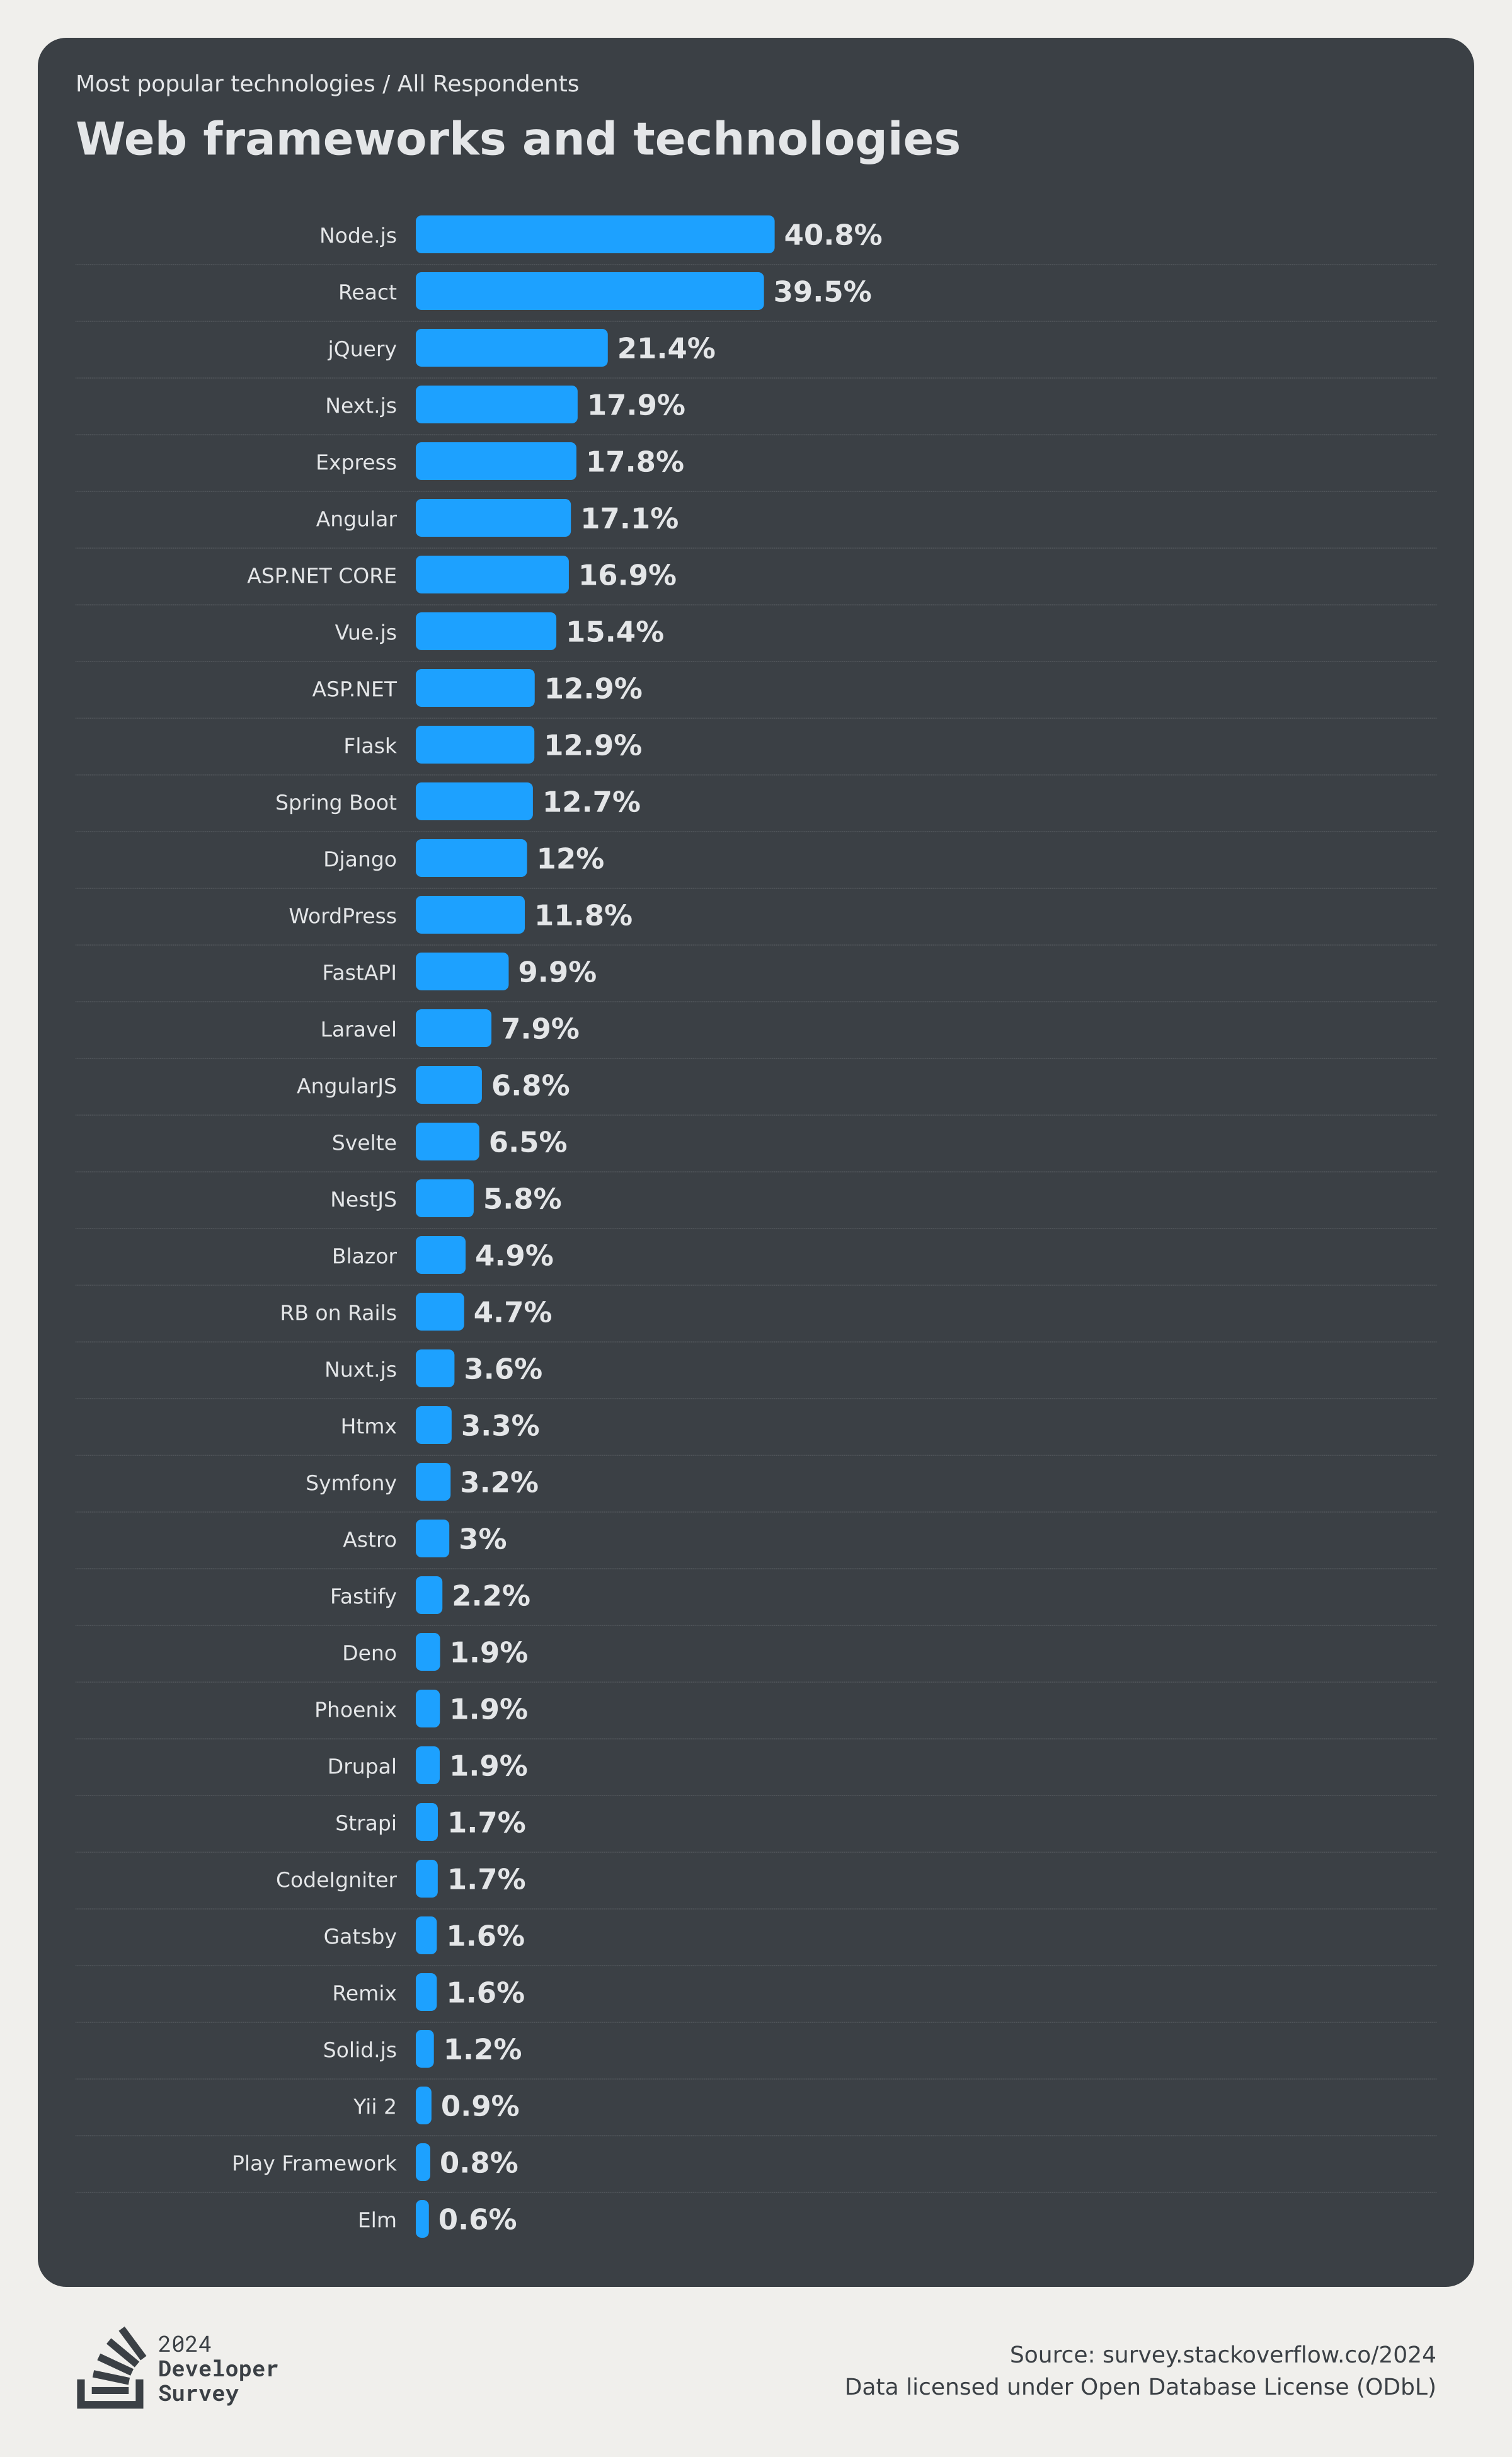
\includegraphics[height=\dimexpr
          \textheight-15\baselineskip-\parskip-.2em-
        \abovecaptionskip-\belowcaptionskip\relax]{stack-overflow-tech.png}
        \caption{Δημοφιλέστερα Πλαίσια Διαδικτύου και τεχνολογίες του
        2024, \textit{Δανεισμένο από \cite{so2024}}}
      \end{center}
      \label{fig:SO2024FRAMEWORKS}
    \end{figure}

    Τα δεδομένα της εφαρμογής αποθηκεύτηκαν σε μια βάση δεδομένων
    \textlatin{MySQL} \cite{mysql}, μια από τις πιο διαδεδομένες σχεσιακές
    βάσεις δεδομένων \cite{so2024}. Tο εργαλείο της Αντικειμενο-σχεσιακής
    Απεικόνισης \textlatin{(ORM)} που χρησιμοποιήθηκε ήταν το
    \textlatin{Prisma} \cite{prisma}, το οποίο παρέχει την δυνατότητα
    δημιουργίας απλών και ασφαλών ερωτημάτων \textlatin{(queries)} στην
    βάση δεδομένων. To σύστημα διαχείρισης της ταυτότητας των χρηστών
    \textlatin{(authentication)} και των δικαιωμάτων τους
    \textlatin{(authorization)} υλοποιήθηκε με την χρήση της βιβλιοθήκης
    \textlatin{NextAuth.js} \cite{nextauth}.
    \begin{figure}[H]
      \begin{center}
        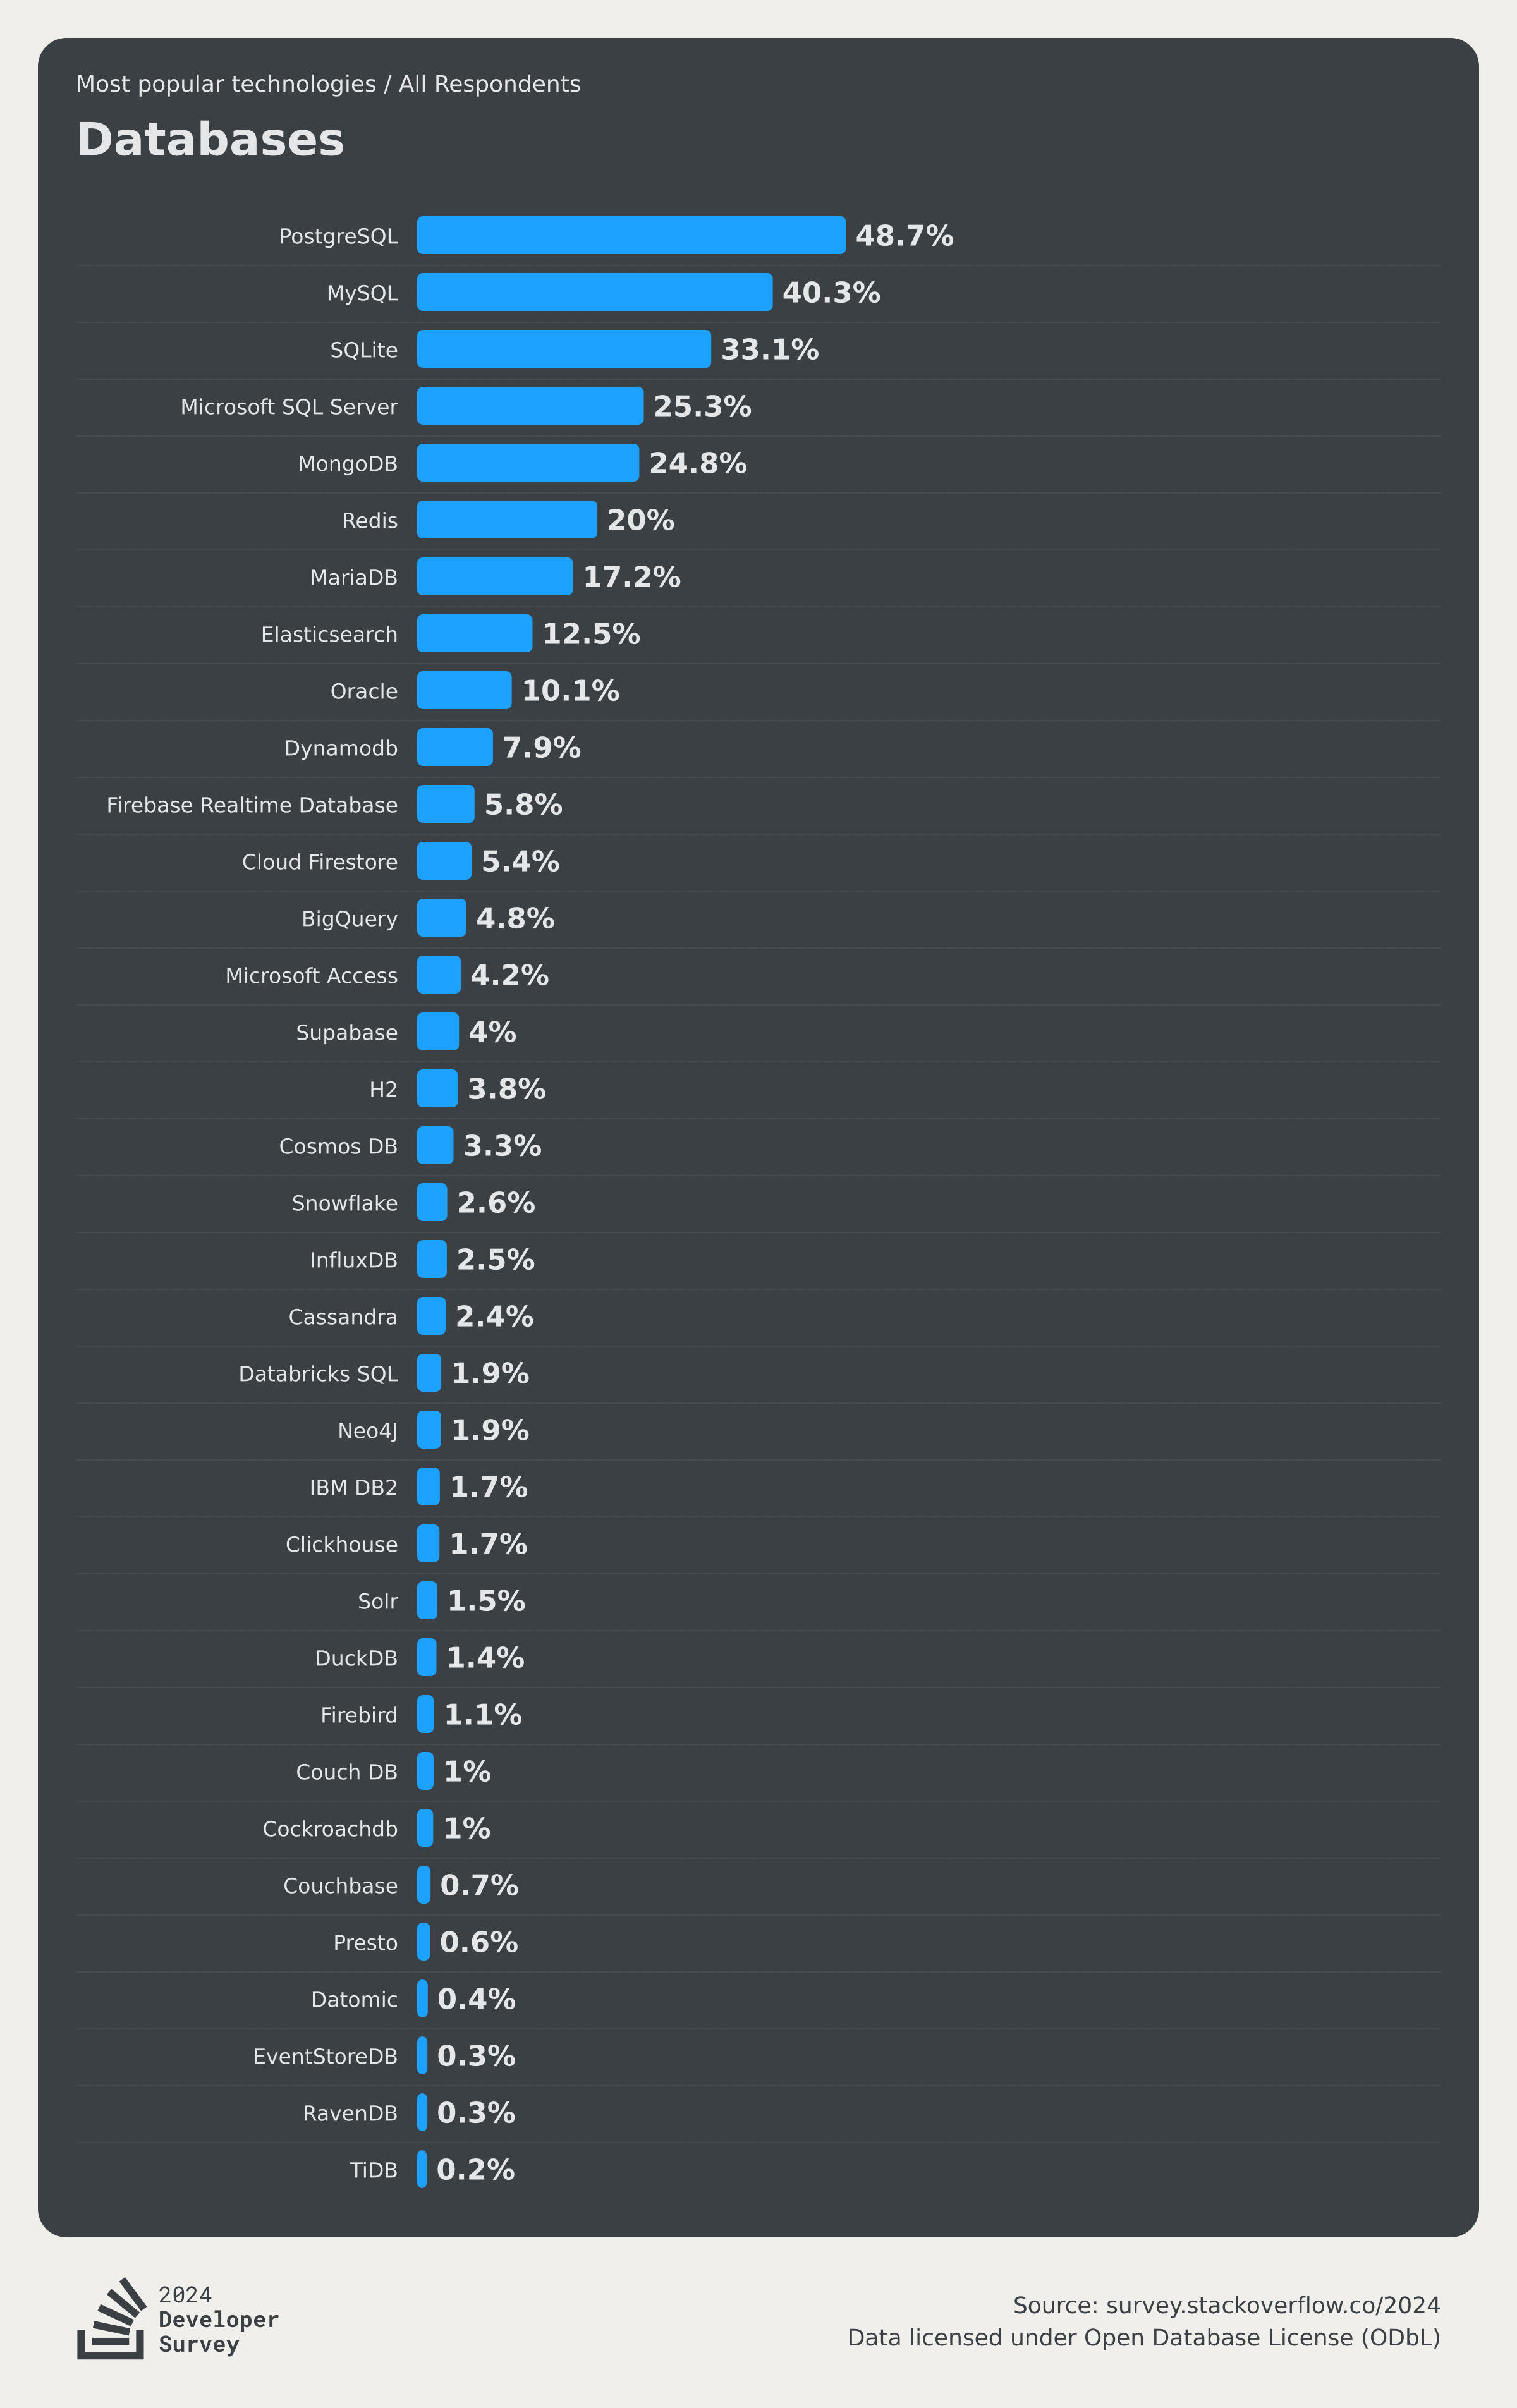
\includegraphics[height=\dimexpr
          \textheight-15\baselineskip-\parskip-.2em-
        \abovecaptionskip-\belowcaptionskip\relax]{stack-overflow-db.png}
        \caption{Δημοφιλέστερες Βάσεις Δεδομένων του 2024,
        \textit{Δανεισμένο από \cite{so2024}}}
      \end{center}
      \label{fig:SO2024DB}
    \end{figure}
  \item
    \textbf{Εμπρόσθια Ανάπτυξη (\textlatin{Frontend Development}):} Η
    εμπρόσθια ανάπτυξη της εφαρμογής έγινε με την χρήση της
    \textlatin{React} \cite{react}, μιας βιβλιοθήκης της
    \textlatin{JavaScript} για την ανάπτυξη διεπαφών χρήστη, την πλέον πιο
    ευρέως γνωστή βιβλιοθήκη \textlatin{Javascript} για ανάπτυξη διεπαφών
    χρήστη \cite{so2024}. Συγκεκριμένα, χρησιμοποιήθηκε το πλαίσιο
    εργασίας \textlatin{Next.js} \cite{nextjs}, το οποίο παρέχει
    δυνατότητες όπως την προ-φόρτωση των σελίδων, την δυνατότητα
    δημιουργίας στατικών ιστοσελίδων, και την δυνατότητα δημιουργίας
    δυναμικών ιστοσελίδων, αποτελώντας ένα από τα πιο ευρέως
    χρησιμοποιημένα πλαίσια εργασίας.
  \item
    \textbf{Έλεγχος Λογισμικού (\textlatin{Software Testing}):} Για τον
    έλεγχο της λειτουργίας του παραγόμενου κώδικα, χρησιμοποιήθηκε το
    πλαίσιο εργασίας \textlatin{Jest} \cite{jest}, το οποίο παρέχει την
    δυνατότητα δημιουργίας και εκτέλεσης δοκιμαστικών συνόλων κώδικα, με
    σκοπό την εξασφάλιση της άρτιας λειτουργίας του κώδικα.
    \cite{Jacobson1999,irena2008,swebok2004,miller1981,shaw1990}
\end{itemize}

Η παραπάνω στοίβα ονομάστηκε \textlatin{T3 stack}, έχοντας πλέον
δημιουργήσει μια μεγάλη κοινότητα στον κλάδο της ανάπυτξης ιστότοπων και
της ανάπτυξης λογισμικού. \cite{t3repo}

\begin{figure}[H]
  \begin{center}
    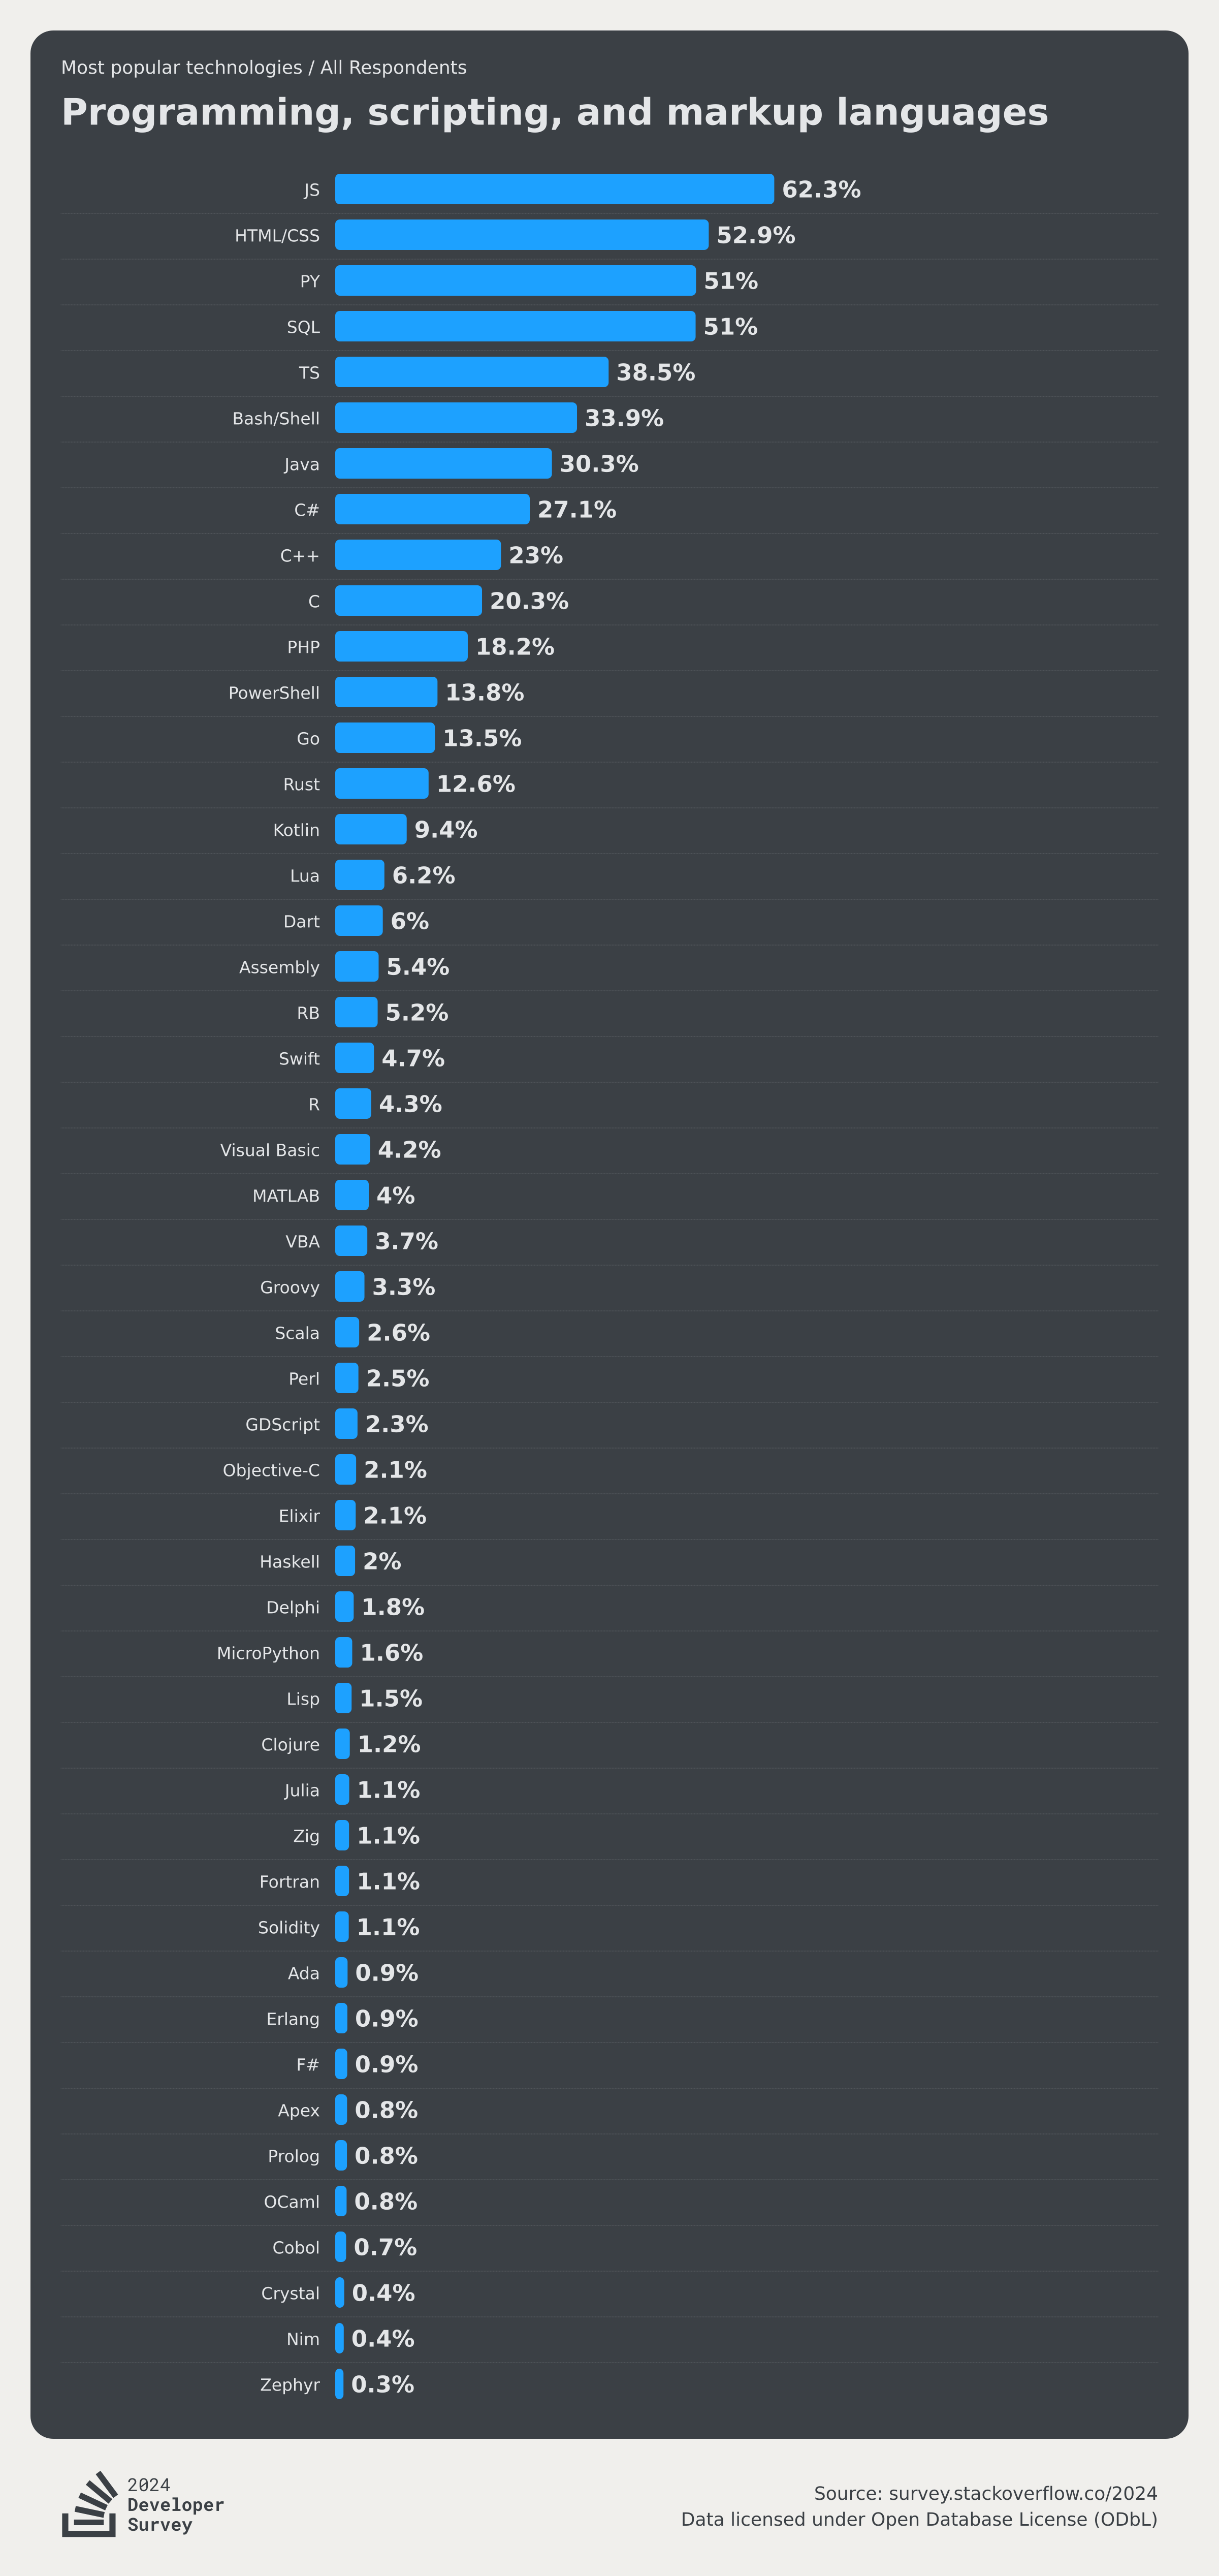
\includegraphics[height=\dimexpr
      \textheight-12\baselineskip-\parskip-.2em-
    \abovecaptionskip-\belowcaptionskip\relax]{stack-overflow-2024-languages.png}
    \caption{Δημοφιλέστερες Γλώσσες Προγραμματισμού του 2024,
    \textit{Δανεισμένο από \cite{so2024}}}
  \end{center}
  \label{fig:SO2024LANGS}
\end{figure}

\section{Επιλογή Περιβάλλοντος Ανάπτυξης }

Η επιλογή του περιβάλλοντος ανάπτυξης έγινε με βάση την ευκολία στην
ενσωμάτωση του \textlatin{GitHub Copilot} και την ευρεία χρήση του
περιβάλλοντος ανάπτυξης. Η επιλογή έγινε στο \textlatin{Visual Studio
Code} \cite{vscode}, το πιο δημοφιλές, σύμφωνα με την επισκόπηση του
\textlatin{Stack Overflow} του 2024, περιβάλλον ανάπτυξης
\cite{so2024}. To \textlatin{Visual Studio Code} είναι ένα περιβάλλον
ανάπτυξης ανεπτυγμένο από την \textlatin{Microsoft} το 2015,
χρησιμοποιώντας την ανοιχτού κώδικα πλατφόρμα \textlatin{Code - OSS}. To
\textlatin{GitHub Copilot Chat} ήταν για πρώτη φορά διαθέσιμο στο
\textlatin{Visual Studio Code} μέσω της ομώνυμης επέκτασης.
\cite{copilotchatrepo}

\begin{figure}[H]
  \begin{center}
    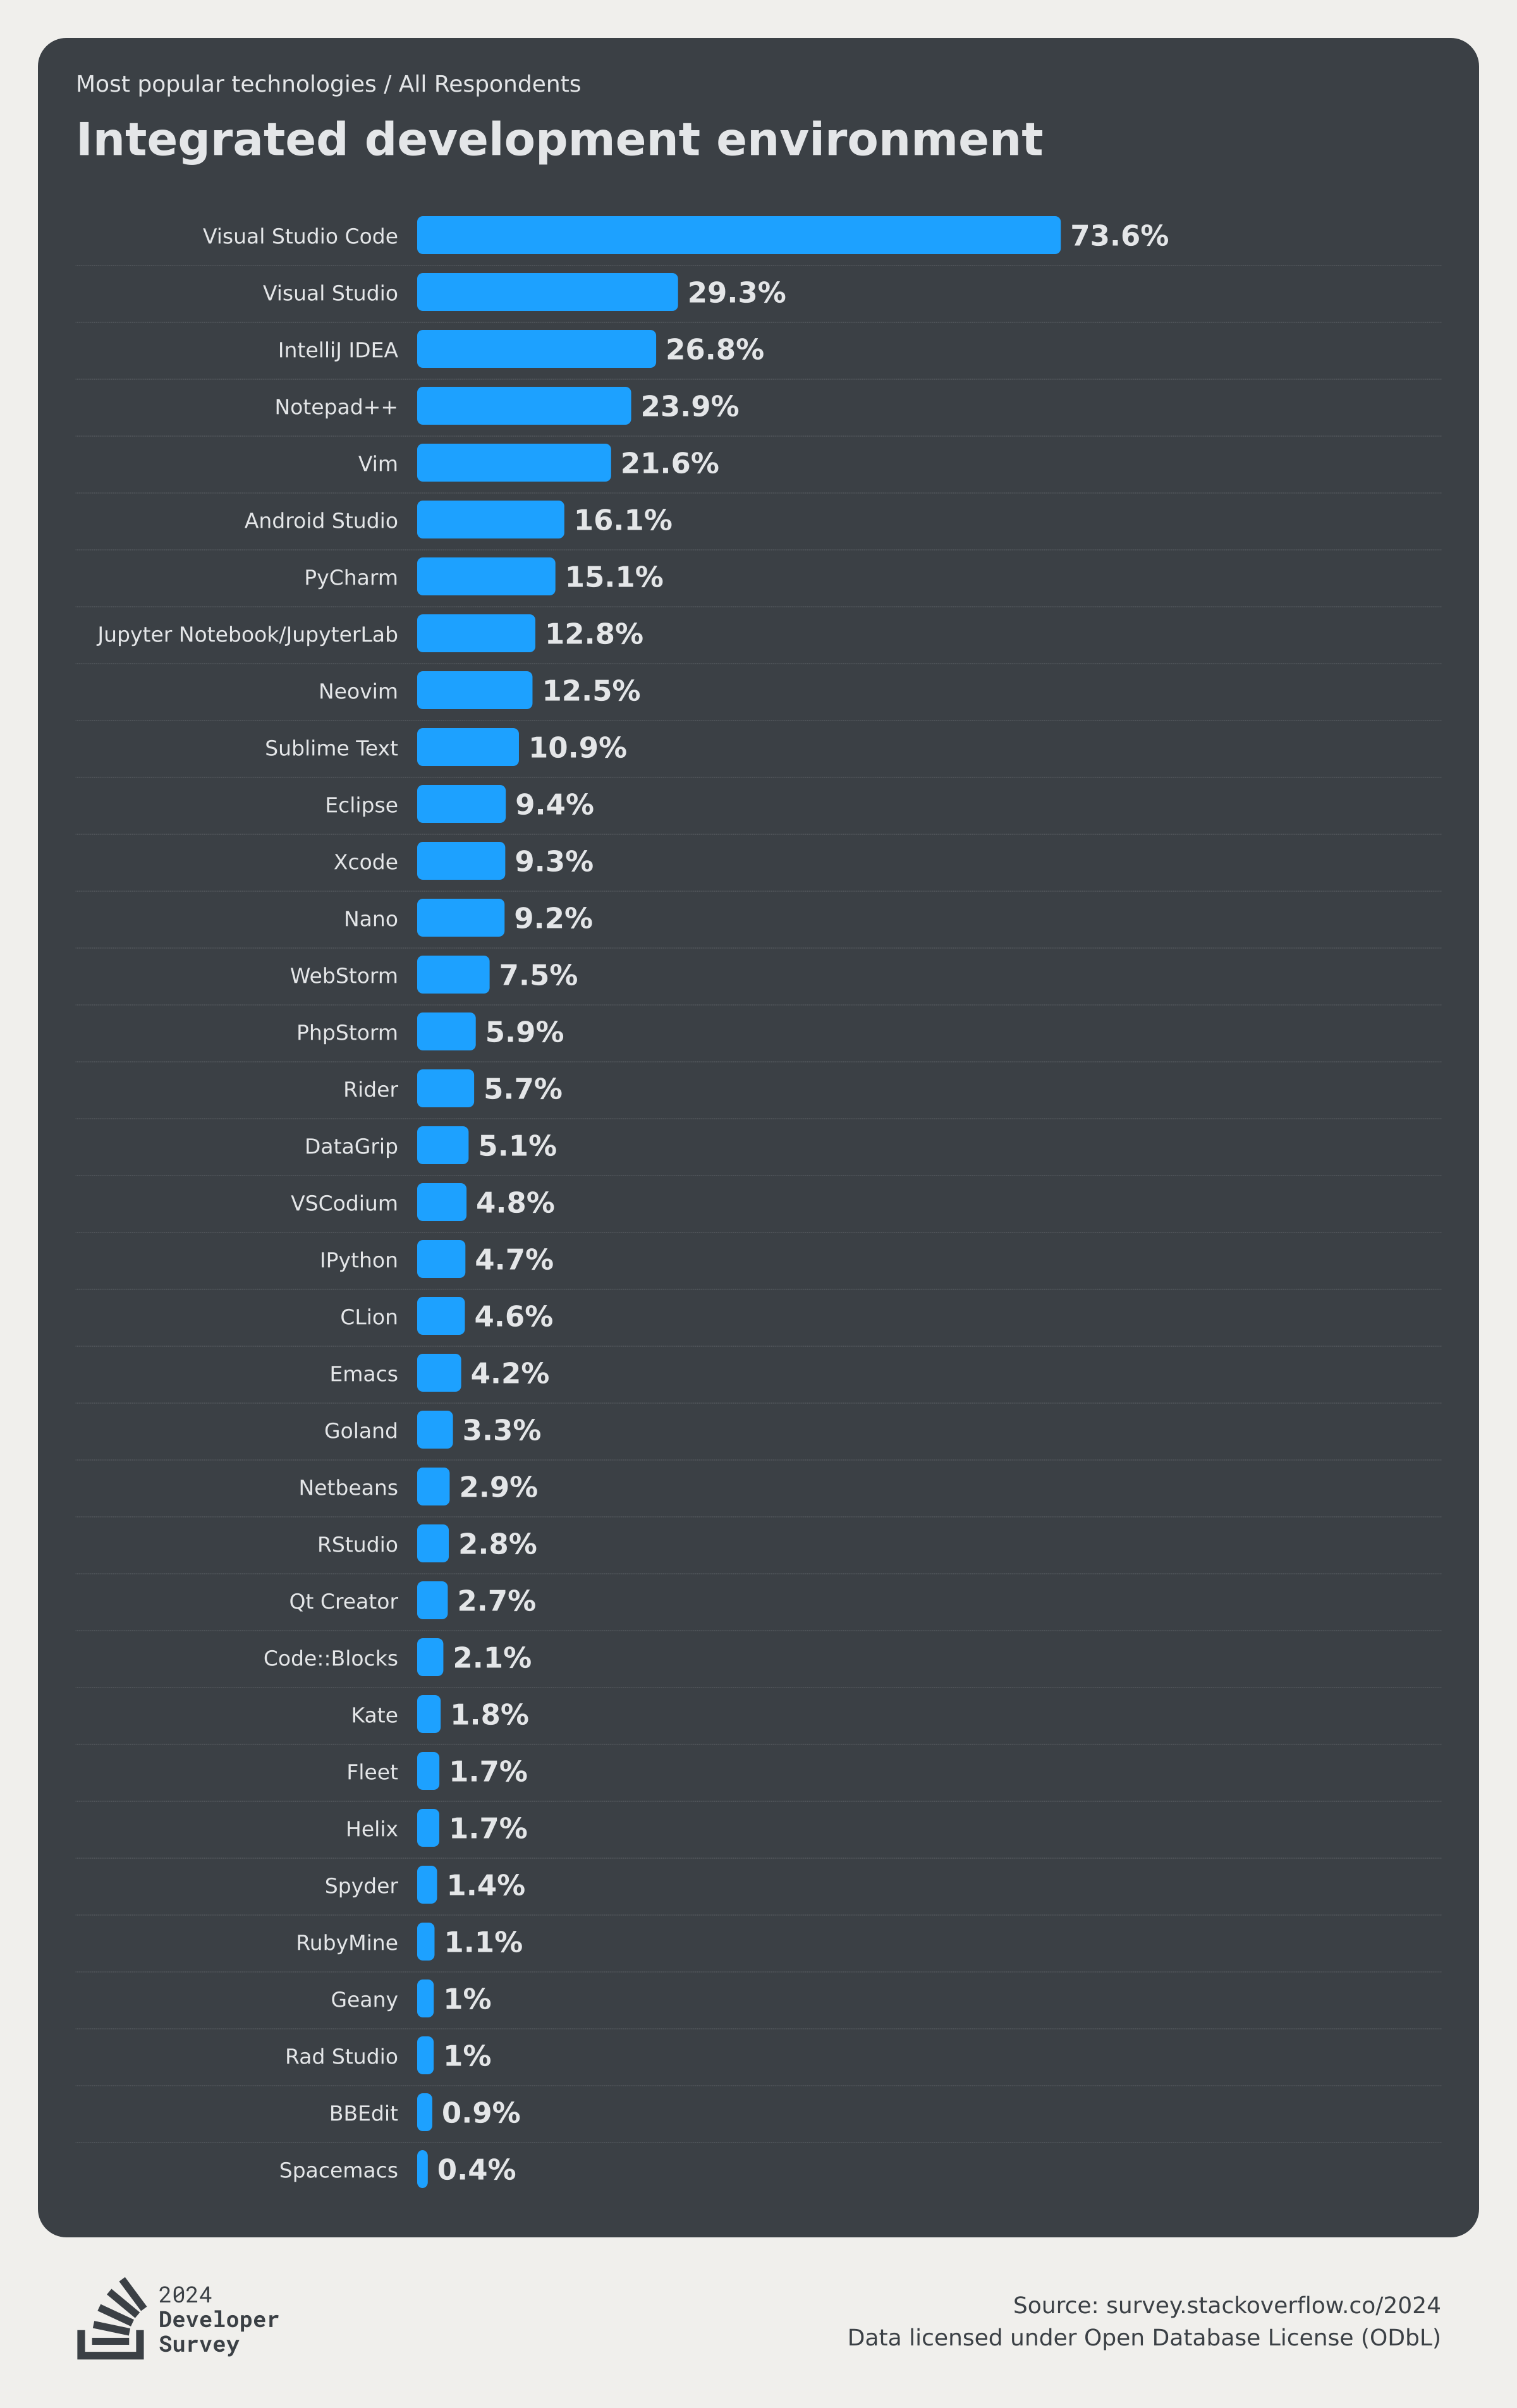
\includegraphics[height=\dimexpr
      \textheight-15\baselineskip-\parskip-.2em-
    \abovecaptionskip-\belowcaptionskip\relax]{stack-overflow-ide.png}
    \caption{Δημοφιλέστερα περιβάλλοντα ανάπτυξης (\textlatin{IDE}) του
    2024, \textit{Δανεισμένο από \cite{so2024}}}
  \end{center}
  \label{fig:SO2024IDES}
\end{figure}

\section{Συλλογή Δεδομένων}

Για την συλλογή των δεδομένων, αρχικά δημιουργήθηκε ο σκελετός της βάσης
κώδικα \textlatin{(codebase)}, καθώς και μια λειτουργικότητα της
εφαρμογής, μαζί με τα αντίστοιχα αρχεία ελέγχου της λειρουγίας του
κώδικα. Η λειτουργικότητα που επιλέχθηκε να αναπτυχθεί χωρίς την χρήση
του μοντέλου ήταν αυτής της σειράς του βιντεοπαιχνιδιού
\textlatin{(Franchise)}. Η επιλογή έγινε γιατί η λειτουργικότητα αυτή
ήταν αρκετά απλή, καθώς η σειρά έχει μόνο σχέσεις 1:Μ με οντότητα του
βιντεοπαιχνιδιού \textlatin{(Game)} \ref{fig:rdd}.

Με αυτό τον τρόπο, δημιουργήθηκαν μέθοδοι για την δημιουργία, την
ανάγνωση, την ενημέρωση και την διαγραφή των σειρών του βιντεοπαιχνιδιού
\textlatin{(CRUD)}, καθώς και έλεγχοι για την σωστή εκτέλεση αυτών, με
βάση την ταυτοποίηση και των δικαιωμάτων των χρηστών. Σκοπός της
προεργασίας αυτής ήταν η αξιολόγηση του κατά πόσο το μοντέλο θα
ακολουθούσε τις κατευθυντήριες γραμμές που ορίστηκαν από τον
προγραμματιστή.

\subsection{Διαχείρηση Ποιότητας Κώδικα}
Για να διασφαλιστεί η ποιότητα του κώδικα του σκελετού της βάσης
κώδικα, χρησιμοποιήθηκε το εργαλείο διαχείρισης ποιότητας κώδικα
\tl{Cyclopt}. Το \tl{Cyclopt} αξιολογεί μια βάση κώδικα
με βάση διάφορες μετρικές, παρέχοντας πληροφορίες για τη συνολική
υγεία και συντηρησιμότητα του λογισμικού \cite{cyclopt}.
Το \tl{Cyclopt} αξιολογεί μια βάση κώδικα χρησιμοποιώντας διάφορες
βασικές μετρικές:

\begin{itemize}
  \item Συντηρησιμότητα: Αυτή η μετρική αξιολογεί πόσο εύκολο είναι
    να τροποποιηθεί, να ενημερωθεί και να επεκταθεί η βάση κώδικα με
    την πάροδο του χρόνου. Λαμβάνει υπόψη παράγοντες όπως η δομή του
    κώδικα σε επιμέρους λειτουργικές μονάδες και τον βαθμό
    αλληλεξάρτησης μεταξύ διαφορετικών τμημάτων του κώδικα
    \cite{maintainability}.

  \item Αναγνωσιμότητα: Αυτή η μετρική αξιολογεί πόσο εύκολα οι
    ανθρώπινοι προγραμματιστές μπορούν να κατανοήσουν και να
    ερμηνεύσουν τον κώδικα. Λαμβάνει υπόψη παράγοντες όπως οι
    συμβάσεις ονοματοδοσίας, η δομή του κώδικα και η τεκμηρίωση
    \cite{readability}.
  \item Ευπάθειες Ασφαλείας: Το \tl{Cyclopt} σαρώνει τον κώδικα για
    πιθανές αδυναμίες ασφαλείας και κοινές ευπάθειες, βοηθώντας στον
    εντοπισμό και την αντιμετώπιση των κινδύνων νωρίς στη διαδικασία
    ανάπτυξης \cite{security_vulnerabilities}.
  \item Πολυπλοκότητα: Το εργαλείο χρησιμοποιεί δύο κύρια μέτρα για
    την αξιολόγηση της πολυπλοκότητας του κώδικα:
    \begin{enumerate}
      \item Πολυπλοκότητα \tl{Halstead}: Αυτή η μετρική, που
        αναπτύχθηκε από τον \tl{Maurice Howard Halstead}, μετρά την
        πολυπλοκότητα ενός προγράμματος με βάση τον αριθμό των
        τελεστών και των τελεστέων στον κώδικα \cite{halstead}.
      \item Πολυπλοκότητα   \tl{McCabe}: Aυτή η μετρική ποσοτικοποιεί
        τον αριθμό των
        γραμμικά ανεξάρτητων μονοπατιών μέσα από τον πηγαίο κώδικα
        ενός προγράμματος \cite{mccabe}.
      \end{enumarate}
  \end{itemize}
  Χρησιμοποιώντας το \tl{Cyclopt} στη διαδικασία ανάπτυξης,
  στόχος ήταν η διατήρηση υψηλών προτύπων ποιότητας κώδικα καθ' όλη
  τη διάρκεια του έργου, διασφαλίζοντας ότι η βάση κώδικα παραμένει
  συντηρήσιμη, αναγνώσιμη και ασφαλής καθώς αυξάνεται σε πολυπλοκότητα.
  \subsection{Διαδικασία Συλλογής Δεδομένων}

  Για την καλύτερη μορφή και κατηγοριοποίηση των δεδομένων, η κάθε
  προτροπή χωρίστηκε σε τέσσερις (4) κατηγορίες, με βάση τo είδος της:

  \begin{itemize}
    \item
      \textbf{Γλώσσας (\textlatin{Language})}: Προτροπές που αφορούν
      ερωτήσεις για την γλώσσα προγραμματισμού (συντακτικό, δομή).
    \item
      \textbf{Πίσω Ανάπτυξης (\textlatin{Backend})}: Προτροπές που αφορούν
      ερωτήσεις για την ανάπτυξη του \textlatin{API} της εφαρμογής.
    \item
      \textbf{Ελέγχου (\textlatin{Testing})}: Προτροπές που αφορούν
      ερωτήσεις για την ανάπτυξη ελέγχου για τις μεθόδους που έχουν γραφτεί.
    \item
      \textbf{Άλλες}: Προτροπές που αφορούν ερωτήσεις που δεν σχετίζονται με
      την συγγραφή κώδικα (για την λειτουργικότητα του \textlatin{GitHub
        Copilot}, για την δομή των απαντήσεών του, τυχόν λάθη από πλευρά του
      προγραμματιστή κατά την σύνταξη της προτροπής).
  \end{itemize}

  Πέρα από την αρχική κατηγοριοποίηση των προτροπών, η κάθε προτροπή
  επίσης κατηγοριοποίηθηκε περαιτέρω, με το κάθε θέμα της ερώτησης, όπως
  για παράδειγμα ανάπτυξη των μεθόδων που αφορούσαν μια οντότητα της
  εφαρμογής και ανάπτυξη ελέγχων αυτών των μεθόδων, εκ των οποίων ελέγχων
  χωρίστηκαν σε \textlatin{Integration Tests} (έλεγχοι συμβατότητας) και
  σε \textlatin{Unit Tests} (έλεγχοι μονάδας) \cite{jamilTesting,
  Kathiriya}. Οι διαφορές μεταξύ των δύο είναι οι εξής:
  \begin{itemize}
    \item
      \textbf{\textlatin{Unit Testing} (Έλεγχος Μονάδας)}: Το
      \textlatin{Unit Testing} επικεντρώνεται στον έλεγχο μεμονωμένων
      κομματιών κώδικα, συνήθως μεθόδων ή συναρτήσεων, σε απομόνωση.
      Στοχεύει στην επαλήθευση ότι κάθε μονάδα του λογισμικού λειτουργεί
      σωστά.
    \item
      \textbf{\textlatin{Integration Testing} (Έλεγχος Συμβατότητας)}: Το
      \textlatin{Integration Testing} εξετάζει πώς διαφορετικά μέρη του
      συστήματος λειτουργούν μαζί. Ελέγχει την αλληλεπίδραση μεταξύ
      διαφορετικών μονάδων ή συστατικών για να διασφαλίσει ότι συνεργάζονται
      σωστά ως σύνολο. Η ειδοποιός διαφορά είναι ότι το \textlatin{Unit
      Testing} εστιάζει σε μεμονωμένα κομμάτια κώδικα, ενώ το
      \textlatin{Integration Testing} εξετάζει πώς αυτά τα κομμάτια
      συνεργάζονται. \cite{patton2005software}
  \end{itemize}

  Για την συλλογή των δεδομένων, δημιουργήθηκε μια περσόνα ενός
  προγραμματιστή για το μοντέλο \cite{zhou2024sotopia,AitBaha2023,
  xu2023expertprompting}, με τους κανόνες να ακολουθεί κάθε του απάντηση
  μια συγκεκριμένη δομή. Ζητήθηκε από το μοντέλο να αρχίζει κάθε μήνυμα με
  το θέμα της ερώτησης, τον τύπο της ερώτησης και έναν άριθμο που
  αναπαριστά την σειρά της ερώτησης για το συγκεκριμένο θέμα. Στη
  συνέχεια, ζητήθηκε από το μοντέλο να βάζει σχόλια στον κώδικα που
  πάραγε, υποδεικνύοντας την αρχή και το τέλος του παραγόμενου κώδικα, με
  τη μορφή \textlatin{\textit{BEGIN\_COPILOT\_CODE / END\_COPILOT\_CODE}}.
  Τέλος, ζητήθηκε από το μοντέλο να παράγει κώδικα που να ακολουθεί τις
  κατευθυντήριες γραμμές που ορίστηκαν από τον προγραμματιστή.

  \begin{figure}[H]
    \begin{center}
      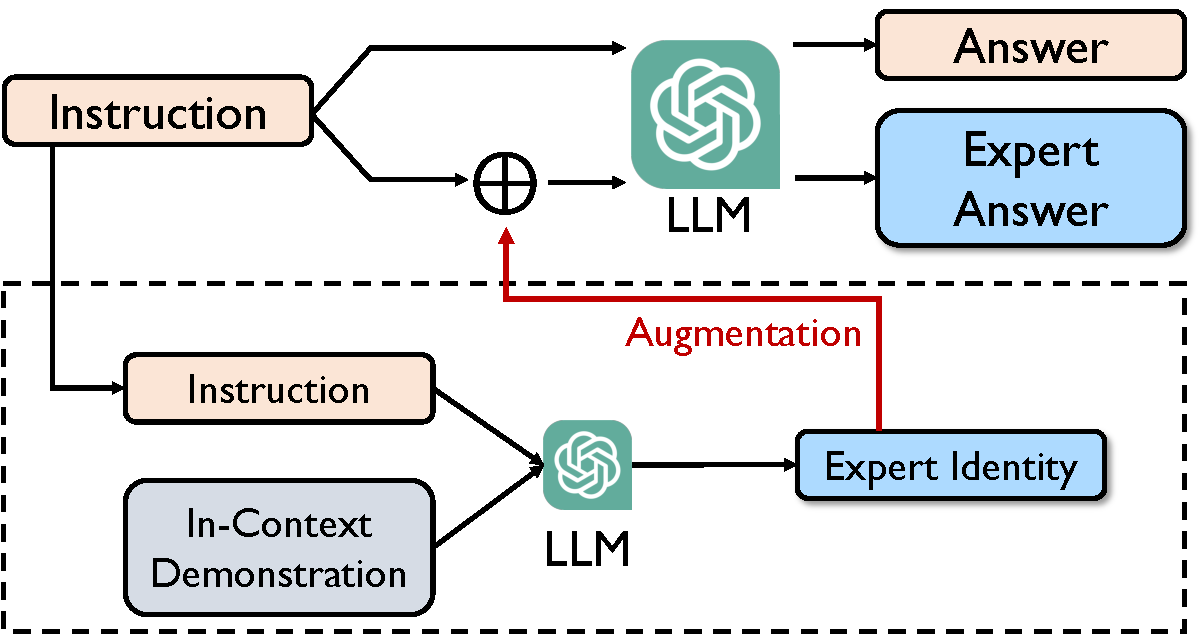
\includegraphics[width=\textwidth]{ExpertPrompting.pdf}
      \caption{Η μεθοδολογία δημιουργίας περσόνας για το μοντέλο,
      \textit{Δανεισμένο από \cite{xu2023expertprompting}} }
    \end{center}
    \label{fig:ExpertPrompting}
  \end{figure}

  \begin{figure}[H]
    \begin{center}
      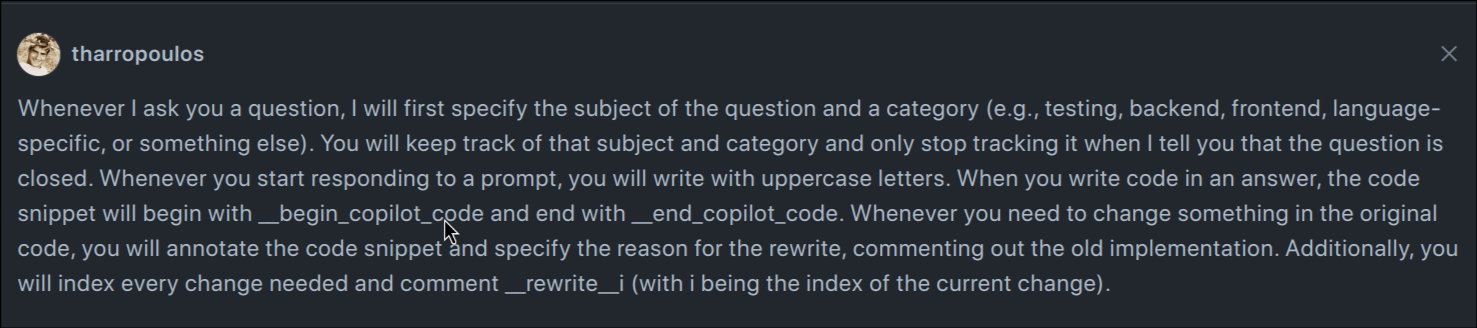
\includegraphics[width=\textwidth]{persona.png}
      \caption{Η προτροπή που δόθηκε στο μοντέλο για την δημιουργία της
      περσόνας}
    \end{center}
    \label{fig:persona}
  \end{figure}

  Η επιλογή να ζητηθεί από το μοντέλο να υποδεικνύει τον κώδικα που
  παράγει έγινε προκειμένου να συλλεχθούν δεδομένα για την ποιότητα του
  κώδικα που παρήχθη, αλλά και για να καταγραφτούν οι φορές που ο
  προγραμματιστής επενέβη, με σκοπό να διορθώσει λάθη που το μοντέλο
  αδυνατούσε. Η τακτική αυτή προϋπόθετε ότι ο προγραμματιστής και
  χειριστής του μοντέλου θα είχε την δυνατότητα να αντιληθφεί τα λάθη που
  παρήχθησαν από το μοντέλο, και να τα διορθώσει, καθώς και να γνωρίζει
  πώς να προτρέψει το μοντέλο να απαντήσει την επιθυμητή απάντηση. Χωρίς
  αυτήν την απόφαση, το μοντέλο θα παρήγαγε κώδικα ο οποίος δεν θα ήταν
  λειτουργικός, καθώς υπήρχαν συντακτικά λάθη που δεν μπορούσε να
  παρατηρήσει.

  \begin{figure}[H]
    \begin{center}
      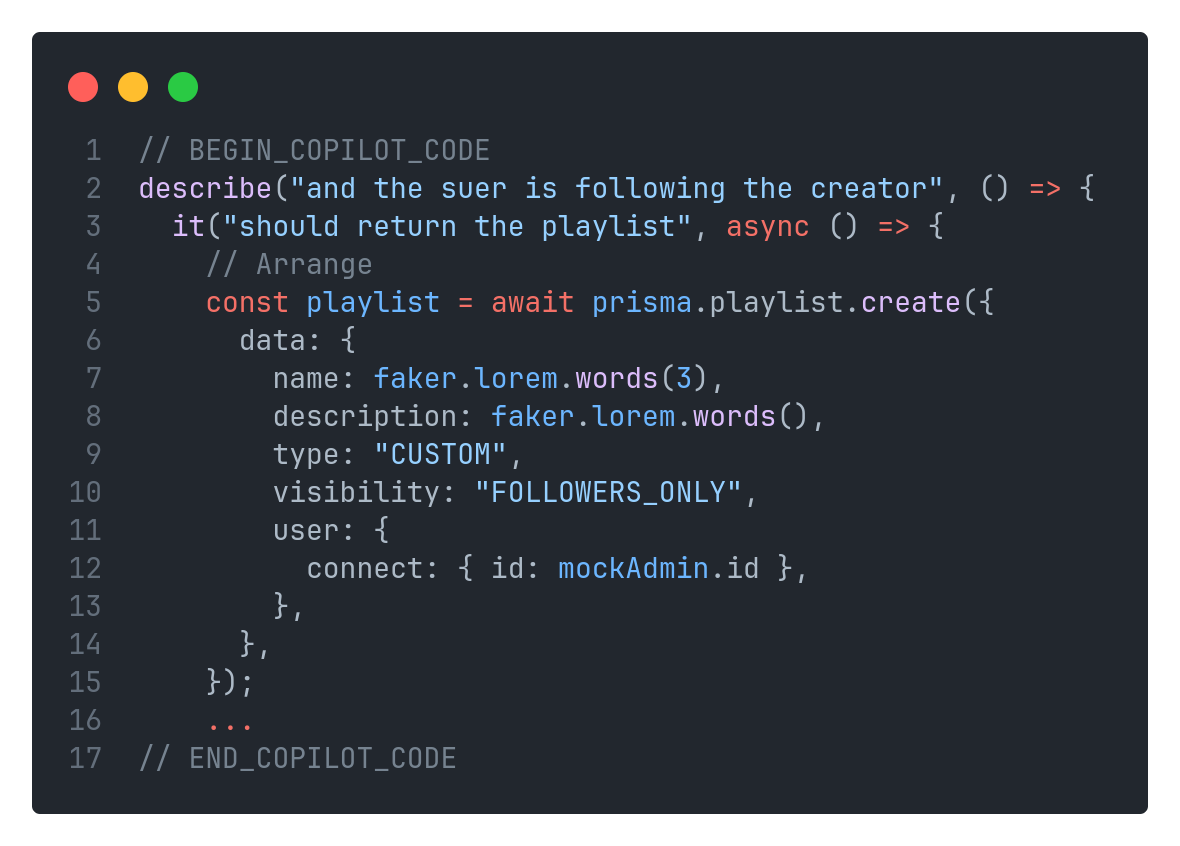
\includegraphics[width=\textwidth]{copilot_code.png}
      \caption{Παράδειγμα κώδικα που παρήχθη από το μοντέλο, με
      ορθογραφικό λάθος}
    \end{center}
    \label{fig:copilotCode}
  \end{figure}

  Η διόρθωση λαθών από τον προγραμματιστή αποτέλεσε έσχατη λύση, καθώς
  πρώτη επιλογή ήταν η αποφυγή συγγραφής κώδικα από τον προγραμματιστή,
  μέσω επισύμανσης των λαθών στο μοντέλο, με την προσδοκία ότι το μοντέλο
  θα διόρθωνε το λάθος χωρίς την ανάγκη επέμβασης του προγραμματιστή. Τα
  λάθη που διορθώθηκαν από το μοντέλο μετά την προτροπή του προγραμματιστή
  σημειώθηκαν με σχόλια με πρόθημα \textlatin{\textit{REWRITE}}, για
  αλλαγές σε μία σειρά κώδικα, ενώ με σχόλια με πρόθημα
  \textlatin{\textit{REVISION}} για αλλαγές σε μικρά κομμάτια κώδικα.

  \begin{figure}[H]
    \begin{center}
      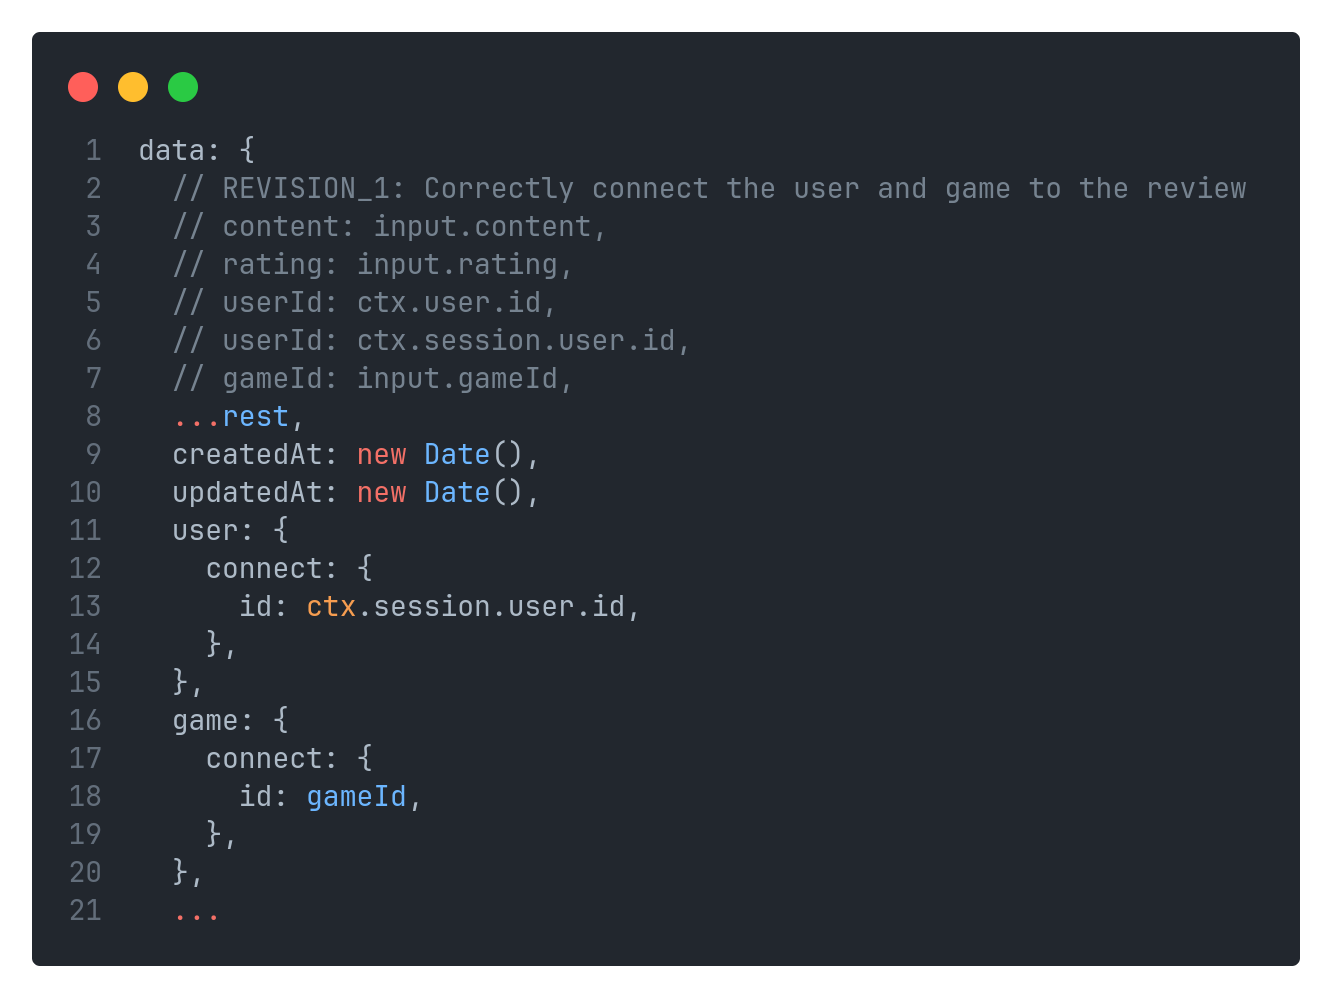
\includegraphics[width=\textwidth]{revision.png}
      \caption{Παράδειγμα διόρθωσης λάθους από το μοντέλο μεγάλης έκτασης,
      μετά την προτροπή του προγραμματιστή}
    \end{center}
    \label{fig:revision}
  \end{figure}

  \begin{figure}[H]
    \begin{center}
      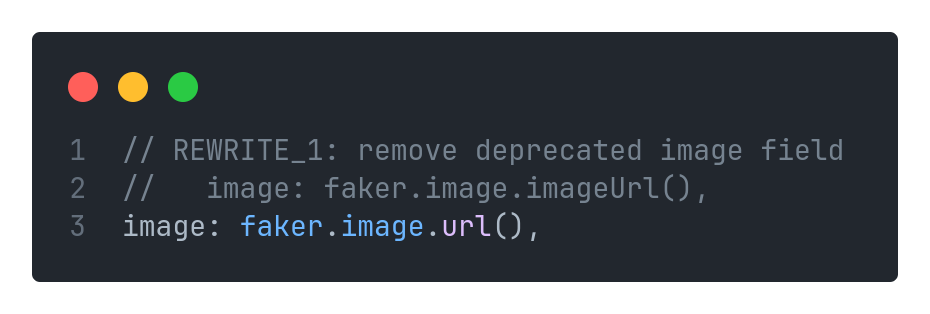
\includegraphics[width=\textwidth]{rewrite.png}
      \caption{Παράδειγμα διόρθωσης λάθους από το μοντέλο μικρής έκτασης,
      μετά την προτροπή του προγραμματιστή}
    \end{center}
    \label{fig:rewrite}
  \end{figure}

  Κατά την διόρθωση λαθών, ο προγραμματιστής άφηνε σχόλια, εξηγώντας το
  λόγο που παρενέβη, με σκοπό την καλύτερη δυνατή τεκμηρίωση, αλλά και την
  εκμάθηση του μοντέλου, με σκοπό την αποφυγή μελλοντικών λαθών,
  σημειώνοντας τα κομμάτια κώδικα με τα σχόλια
  \textlatin{\textit{BEGIN\_NON\_COPILOT\_CODE /
  END\_NON\_COPILOT\_CODE}}.

  \begin{figure}[H]
    \begin{center}
      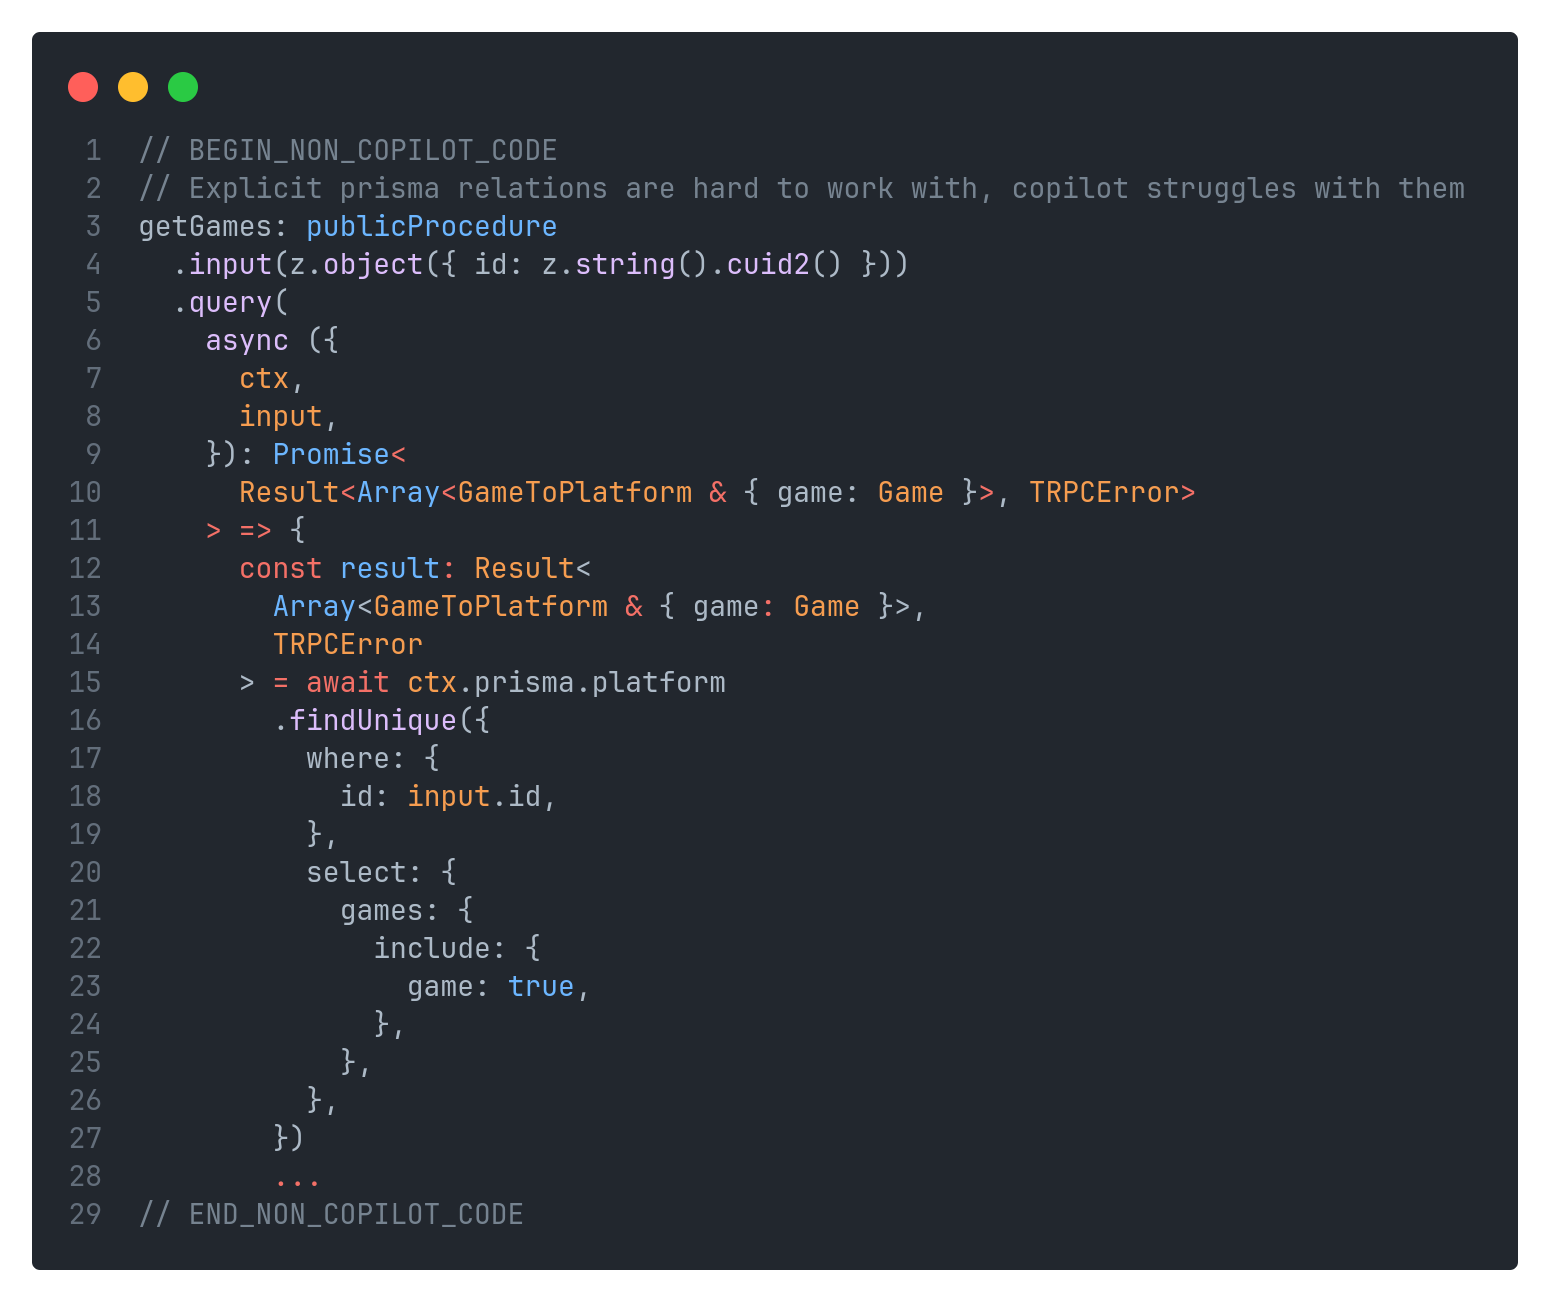
\includegraphics[width=\textwidth]{manual_intervention.png}
      \caption{Παράδειγμα διόρθωσης λάθους από τον προγραμματιστή, μετά
      την αδυναμία του μοντέλου να διορθώσει το λάθος}
    \end{center}
    \label{fig:nonCopilotCode}
  \end{figure}

  Λάθη που διορθώθηκαν μέσω μιας γραμμής (όπως ονομασίες μεταβλητών ή
  συμβόλων), σημειώθηκαν με σχόλια με πρόθημα
  \textlatin{\textit{MANUAL\_REWRITE}}. Επίσης, κατά την χειροκίνητη
  συγγραφή κώδικα, το μοντέλο του \textlatin{GitHub Copilot}, έδινε στον
  προγραμματιστή προτάσεις διόρθωσης του κώδικα. Ορισμένες προτάσεις που
  έλυναν το πρόβλημα, ενσωματώθηκαν στον τελικό κώδικα, σημειώνοντας την
  αρχή και το τέλος του κώδικα που παρήχθη σε πραγματικό χρόνο, μέσω
  σχολίων \textlatin{\textit{BEGIN\_COPILOT\_SUGGESTION /
  END\_COPILOT\_SUGGESTION}}, σημειώνοντας την αρχή και το τέλος του
  προτεινόμενου κομματιού κώδικα.

  \begin{figure}[H]
    \begin{center}
      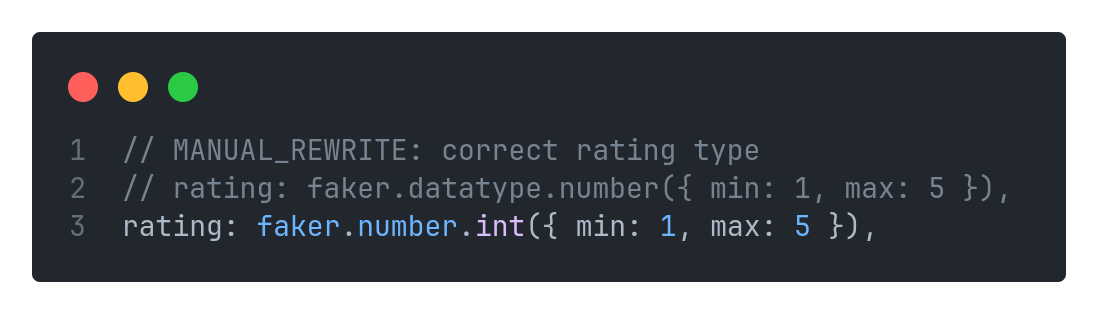
\includegraphics[width=\textwidth]{manual_rewrite.png}
      \caption{Παράδειγμα διόρθωσης λάθους μικρής έκτασης από τον
        προγραμματιστή, μετά την αδυναμία του μοντέλου να διορθώσει το
      λάθος}
    \end{center}
    \label{fig:manualRewrite}
  \end{figure}

  \subsection{Ανάλυση Δεδομένων}

  Μετά την συλλογή των δεδομένων, ακολούθησε η ανάλυσή των ευρημάτων, μέσω
  ενός αναλυτή (\textlatin{lexer} \cite{ball2018}), προκειμένου να
  μετρηθούν τα εξής:

  \begin{itemize}
    \item
      O αριθμός των περιστατικών επέμβασης του προγραμματιστή σε μεγάλες
      εκτάσεις κώδικα
    \item
      Ο αριθμός των περιστατικών επέμβασης του προγραμματιστή σε μικρές
      εκτάσεις κώδικα
    \item
      Ο αριθμός των περιστατικών που το μοντέλο διόρθωσε το λάθος σε μικρές
      εκτάσεις κώδικα
    \item
      Ο αριθμός των περιστατικών που το μοντέλο διόρθωσε μεγαλύτερα λάθη,
      έπειτα από προτροπή του προγραμματιστή
  \end{itemize}

  \begin{table}[h]
    \centering
    \begin{tabular}{lcc}
      \hline
      \textbf{Τύπος} & \textbf{Μικροαλλαγές \textlatin{Copilot}} &
      \textbf{Μικροαλλαγές προγραμματιστή} \\ \hline
      \textlatin{Backend} & 20 & 3 \\
      \textlatin{Integration Tests} & 26 & 7 \\
      \textlatin{Unit Tests} & 32 & 3 \\ \hline
    \end{tabular}
    \caption{Μικροαλλαγές ανά τύπο}
    \label{table:microchanges_by_subject}
  \end{table}

  \begin{table}[h]
    \centering
    \begin{tabular}{lcc}
      \hline
      \textbf{Τύπος} & \textbf{Αλλαγές \textlatin{Copilot}} &
      \textbf{Αλλαγές προγραμματιστή} \\ \hline
      \textlatin{Backend} & 3 & 10 \\
      \textlatin{Integration Tests} & 30 & 14 \\
      \textlatin{Unit Tests} & 4 & 3 \\ \hline
    \end{tabular}
    \caption{Αλλαγές μεγάλης έκτασης ανά τύπο}
    \label{table:major_changes_by_subject}
  \end{table}

  Τα δεδομένα λήφθηκαν μέσα από εικοσιοκτώ (28) αρχεία και πεντακόσιες
  εικοσιπέντε (525) προτροπές και συγκεκριμένα:
  \begin{itemize}
    \item
      Δεκαεπτά (17) αρχεία που αφορούν τον έλεγχο του κώδικα
    \item
      ΄Εντεκα (11) αρχεία που αφορούν την ανάπτυξη του \textlatin{API}
  \end{itemize}

  Παρατίθεται ένα διάγραμμα που αναπαριστά τα αποτελέσματα της ανάλυσης:

  \begin{figure}[htbp]
    \centering
    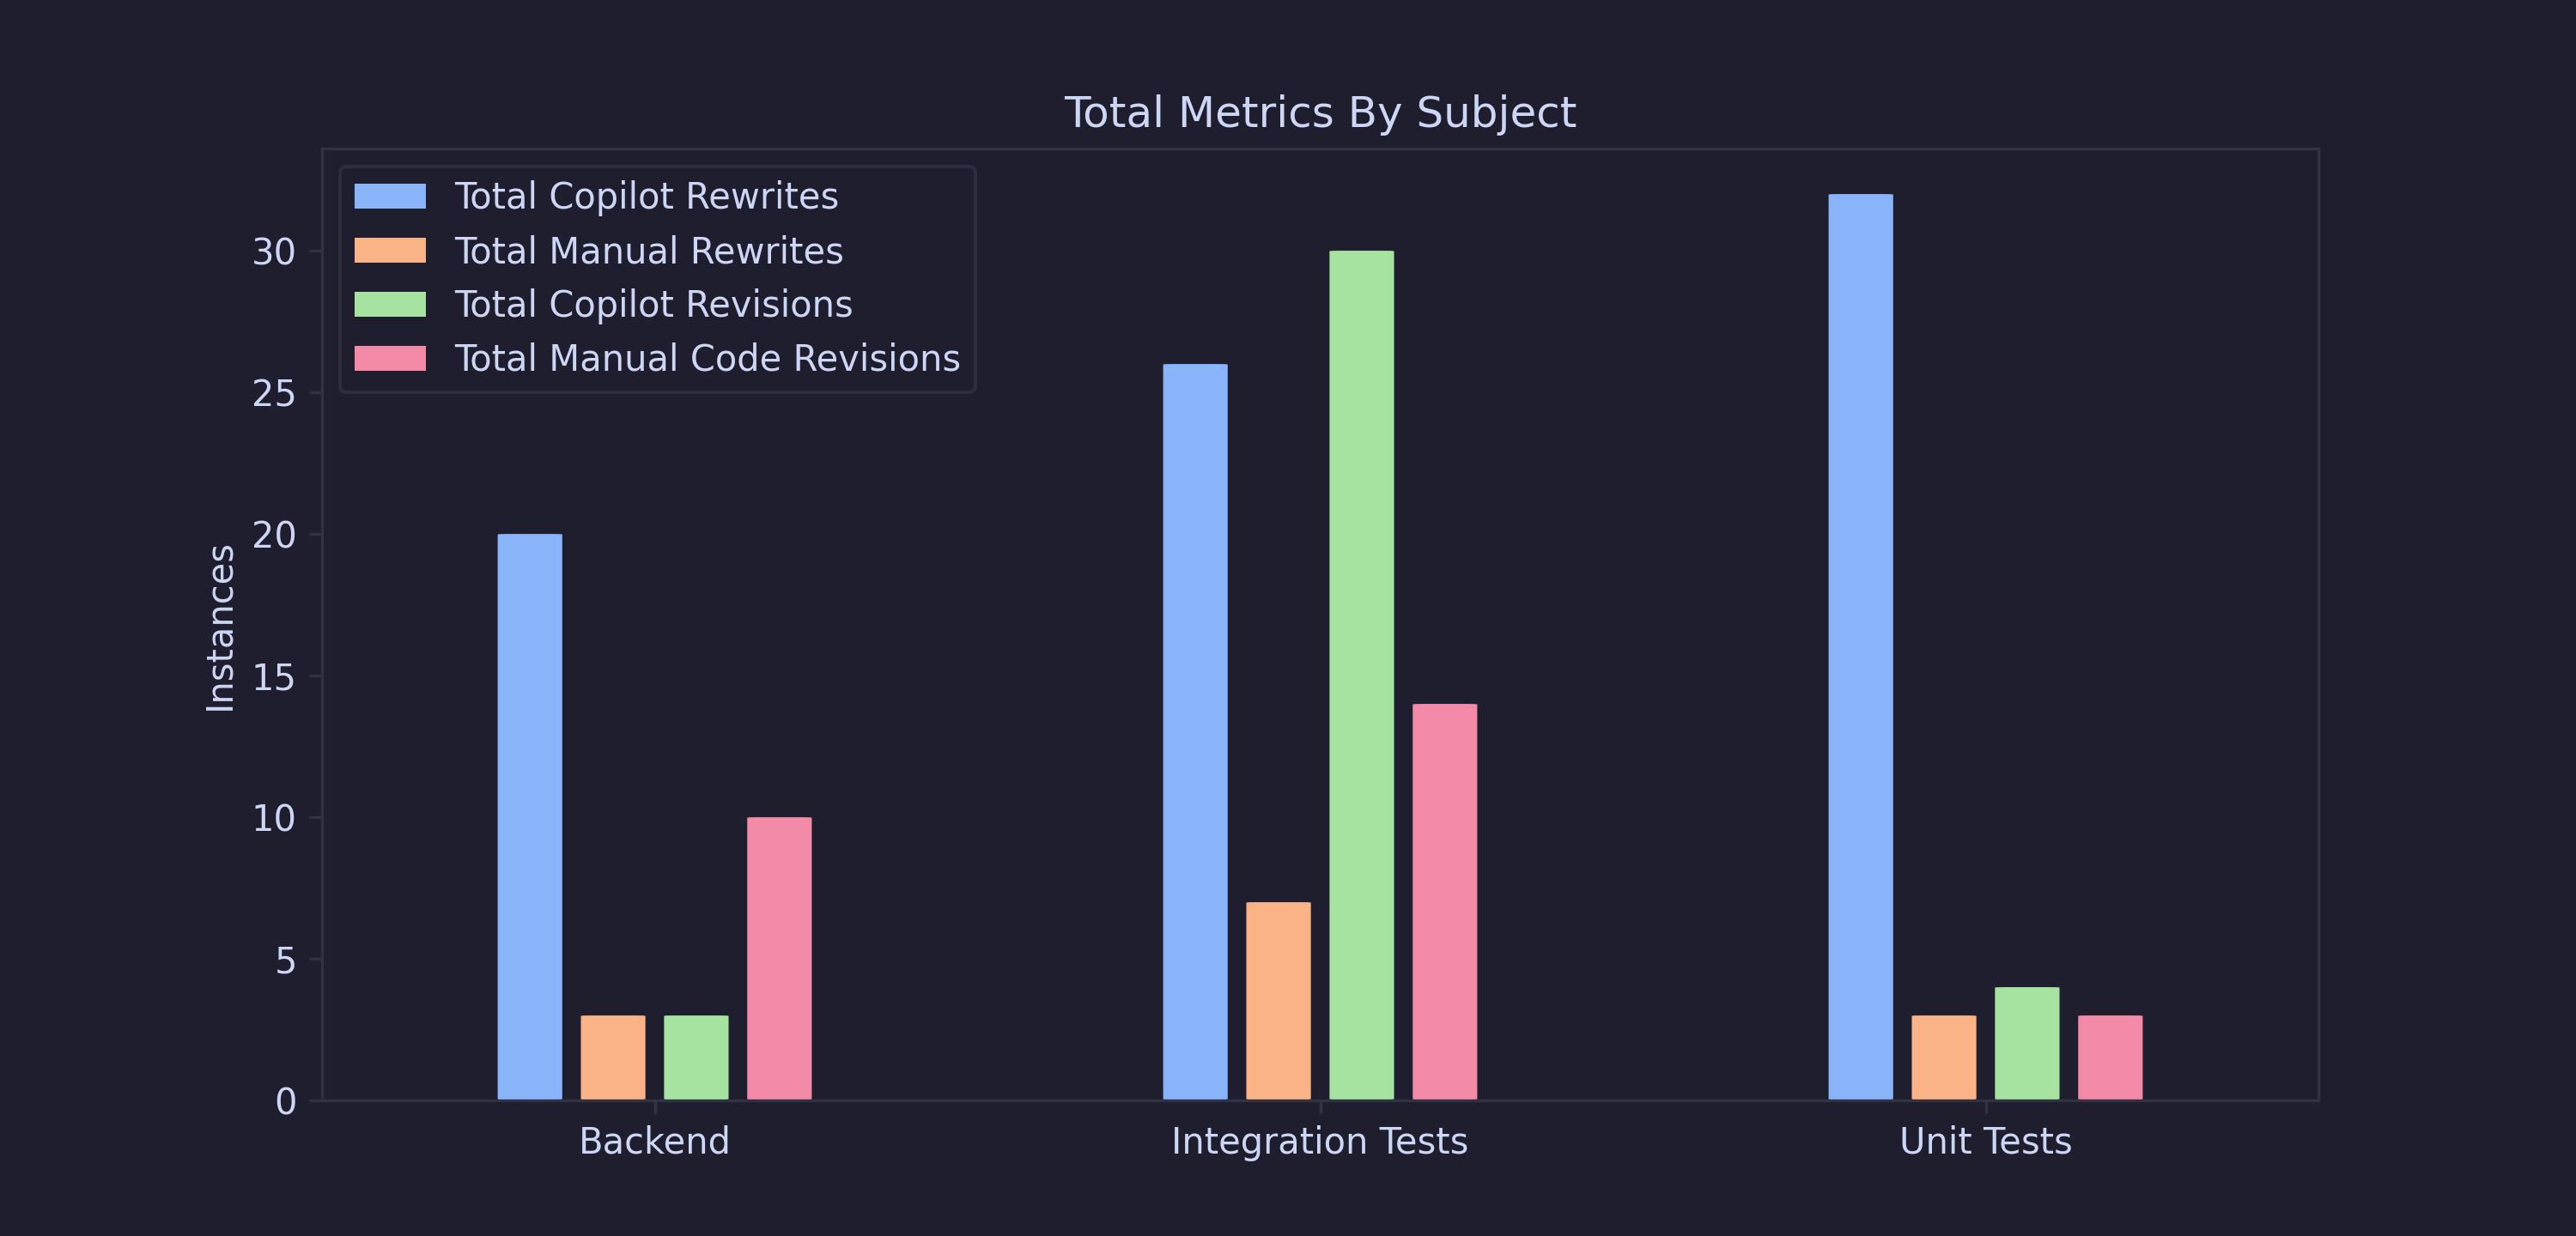
\includegraphics[width=\textwidth]{total_metrics_by_subject.png}
    \caption{Συνολικά μετρικά ανά τύπο}
    \label{fig:totalMetrics}
  \end{figure}

  ΄Οπως φαίνεται από το διάγραμμα \ref{fig:totalMetrics}, οι περισσότεροες
  αλλαγές που πραγματοποιήθηκαν από την πλευρά του μοντέλου έγιναν σε
  μικρές εκτάσεις κώδικα, ενώ οι περισσότερες αλλαγές που
  πραγματοποιήθηκαν από την πλευρά του προγραμματιστή έγιναν σε μεγάλες
  εκτάσεις κώδικα. Σε κάθε τύπο αρχείου παρατηρείται αυτή η τάση, με οτν
  προγραμματιστή να χρειάζεται να επεμβεί πολύ σπανιότερα σε σχέση με το
  μοντέλο και συγκεκριμένα, σε κάθε τύπο αρχείου, οι επεμβάσεις του
  προγραμματιστή για μικρές εκτάσεις κώδικα είναι οι λιγότερες.

  Αξιοσημείωτη επίσης η παρατήρηση ότι στην περίπτωση των αρχειών που
  αφορούσαν το \textlatin{Unit Testing}, οι αλλαγές σε μικρή έκταση κώδικα
  από το μοντέλο ήταν με διαφορά οι περισσότερες, ενώ παράλληλα οι
  υπόλοιπες αλλαγές ήταν ελάχιστες. Αυτό μπορεί να οφείλεται στη χρήση
  βιβλιοθηκών, με βάση τον έλεγχο του κώδικα και πιο συγκεκιμένα αυτή της
  \textlatin{faker.js}\cite{fakerjs}. Η συγκεκριμένη βιβλιοθήκη αφορά την
  δημιουργία ψεύτικων δεδομένων, στο ίδιο πνεύμα με το \textlatin{Lorem
  Ipsum} \cite{lipsum}, αλλά για δεδομένα που αφορούν ένα λογισμικό,
  ΄οπως ημερομηνίες, ονόματα, διευθύνσεις ηλεκτρονικού ταχυδρομίου κ.α.. Η
  βιβλιοθήκη έχει λάβει πολλές εκδόσεις τα τελευταία χρόνια, με αλλαγές
  στον τρόπο που καλούνται οι μέθοδοι του \textlatin{API} της, με
  αποτέλεσμα το μοντέλο να μην μπορεί να ακολουθήσει πάντοτε τις αλλαγές
  αυτές. Σημαντικό να σημειωθεί επίσης ότι το μοντέλο αδυνατούσε να
  παρατηρήσει τις αλλαγές που ζητήθηκαν από τον προγραμματιστή, με
  αποτέλεσμα να ζητηθεί μέσω διαφορετικής προτροπής η αλλαγή της ίδιας
  κλήσης μιας μεθόδου πάνω από μία φορά στο ίδιο αρχείο.

  Στην περίπτωση των αρχείων που αφορούσαν το \textlatin{Backend}, οι
  απαιτούμενες αλλαγές ήταν οι λίγοτερες σε πλήθος, με τη διαφρορά ότι οι
  περισσότερες επεμβάσεις του προγραμματιστή αφορούσαν την γραφή ολόκληρων
  μεθόδων. Η απουσία των απαραίτητων αλλαγών, οφείλεται στο γεγονός ότι η
  βασική λογική πίσω από ένα μεγάλο ποσοστό των μεθόδων αφορά την γραφή
  βασικών \textlatin{CRUD} μεθόδων, οι οποίες είναι προκαθορισμένες και
  δεν απαιτούν αλλαγές. Αυτό έχει ως αποτέλεσμα το μοντέλο να μην
  χρειάζεται να προτρέπεται να αλλάξει την λογική των μεθόδων, αλλά μόνο
  την υλοποίηση τους. Στις περιπτώσεις μεθόδων που επηρέαζαν οντότητες με
  σχέσεις Μ:Ν \cite{prisma2022manytomany}, το μοντέλο του
  \textlatin{GitHub Copilot} αδυνατούσε να ακολουθήσει την λογική, με
  αποτέλεσμα να χρειαστεί να υλοποιηθούν από τον προγραμματιστή.

  Παράδειγμα αποτελεί η περίπτωση της οντότητας του σχολίου. Τα σχόλια
  πραγματοποιούνται σε κριτικές των χρηστών, παρομοίως όπως σε άλλες
  εφαρμογές κοινωνικών δικτύων. Τα σχόλια πραγματοποιούνται σε κριτικές
  των χρηστών, παρομοίως όπως σε άλλες εφαρμογές κοινωνικών δικτύων. Κάθε
  σχόλιο έχει μια σχέση 1:Μ με την κριτική, μια σχέση 1:Μ με τον χρήστη,
  μια σχέση Μ:1 με τις αντιδράσεις τύπου Μου αρέσει \textlatin{(Likes)},
  αλλά μπορεί να έχει και άλλα σχόλια που συνδέονται με αυτό,
  δημιουργώντας ένα "νήμα" \textlatin{(thread)} σχολίων, παρόμοιο
  με έναδιατεταγμένο Κ-οστο δέντρo \cite{gabillon2002access}. Η λογική
  πίσω από την υλοποίηση των μεθόδων που αφορούν τα σχόλια, είναι
  περίπλοκη, με τα ερωτήματα που απαιτούνται να σταλθούν προς στη βάση
  μέσω του \textlatin{Prisma} να είναι πολλά και περίπλοκα. Το μοντέλο του
  \textlatin{GitHub Copilot} αδυνατούσε να ακολουθήσει την λογική, με
  αποτέλεσμα να χρειαστεί να υλοποιηθούν από τον προγραμματιστή.

  \begin{figure}[H]
    \centering
    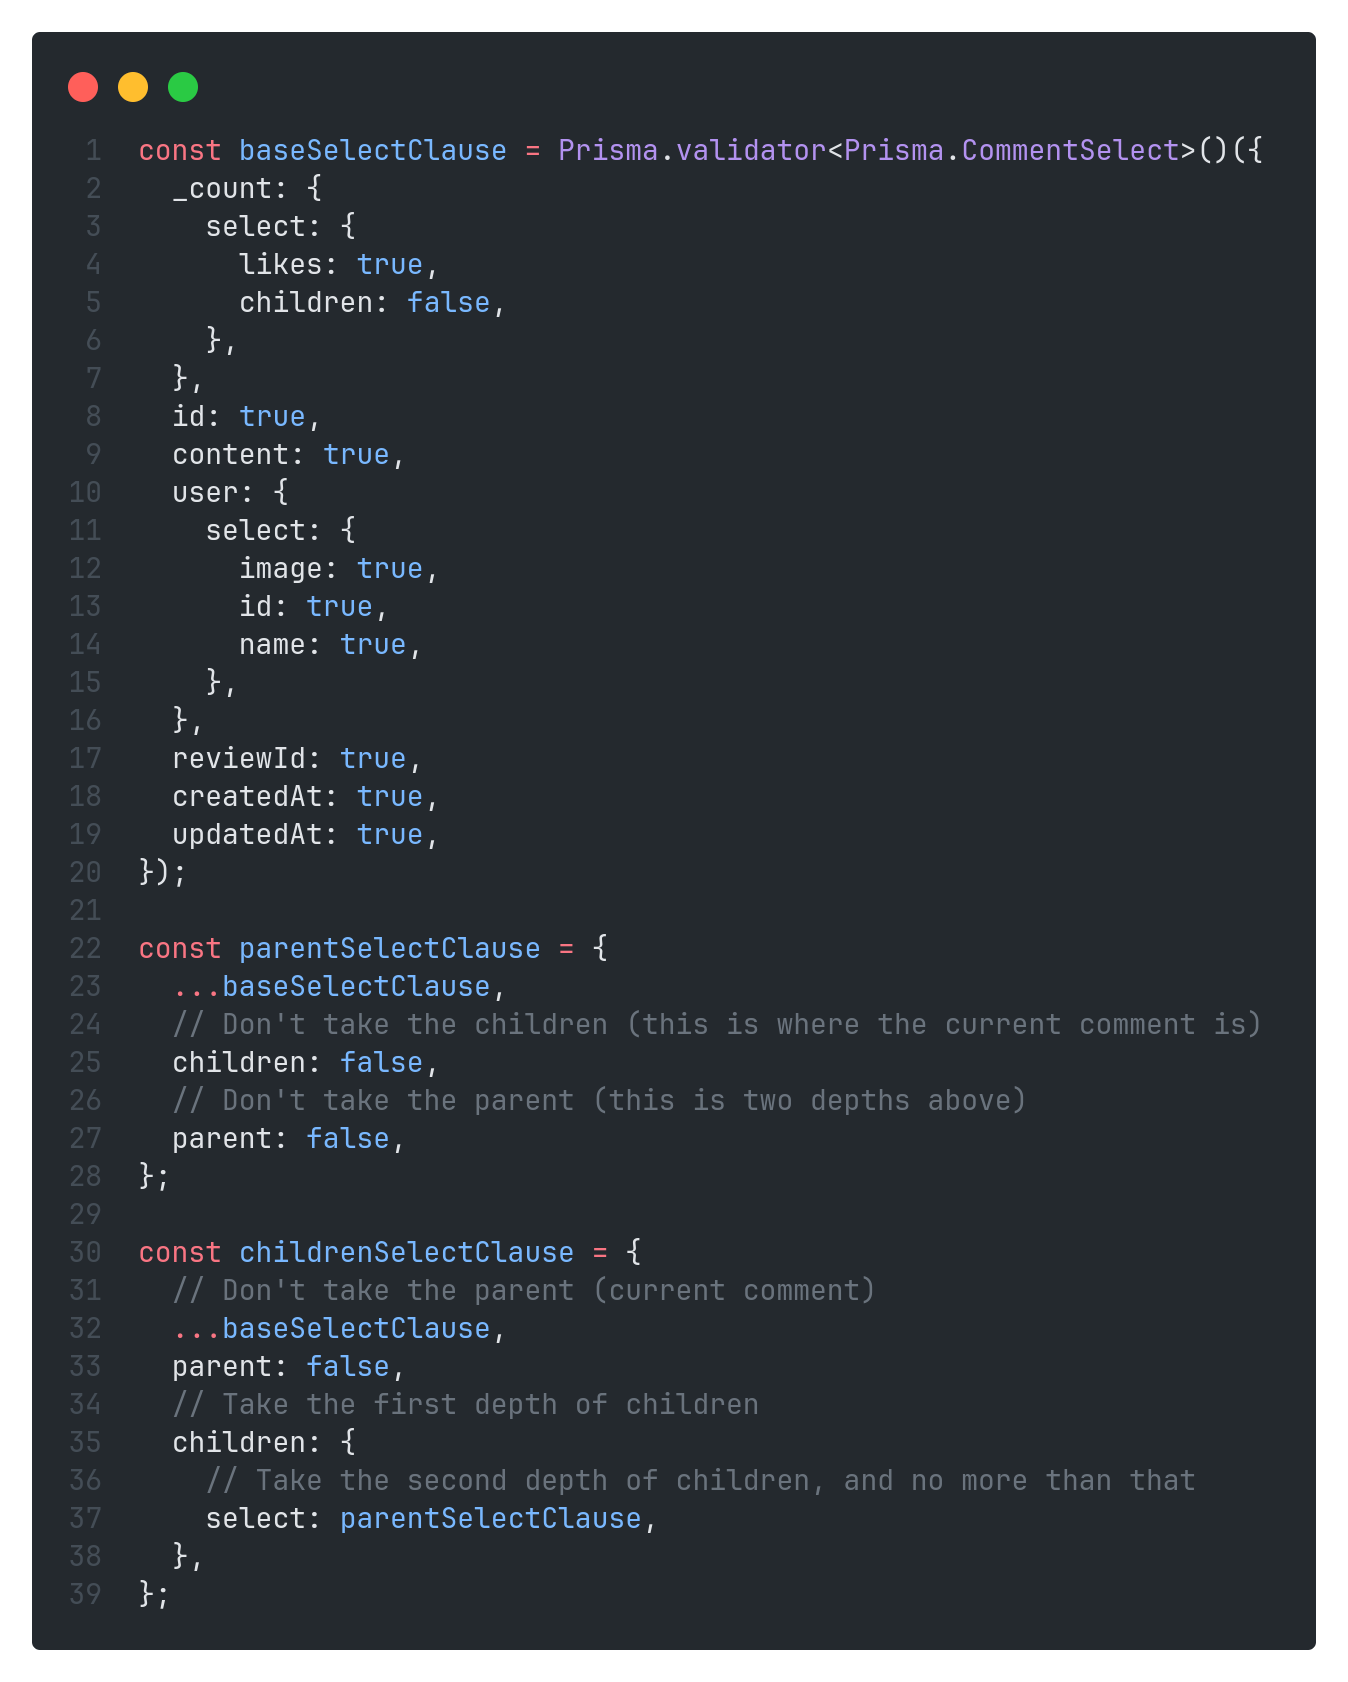
\includegraphics[width=\textwidth]{comment_select_clause.png}
    \caption{Παράδειγμα μεθόδου που αφορά τα σχόλια, με πολλαπλές
    σχέσεις Μ:Ν}
    \label{fig:commentSelectClause}
  \end{figure}

  \begin{figure}[H]
    \begin{center}
      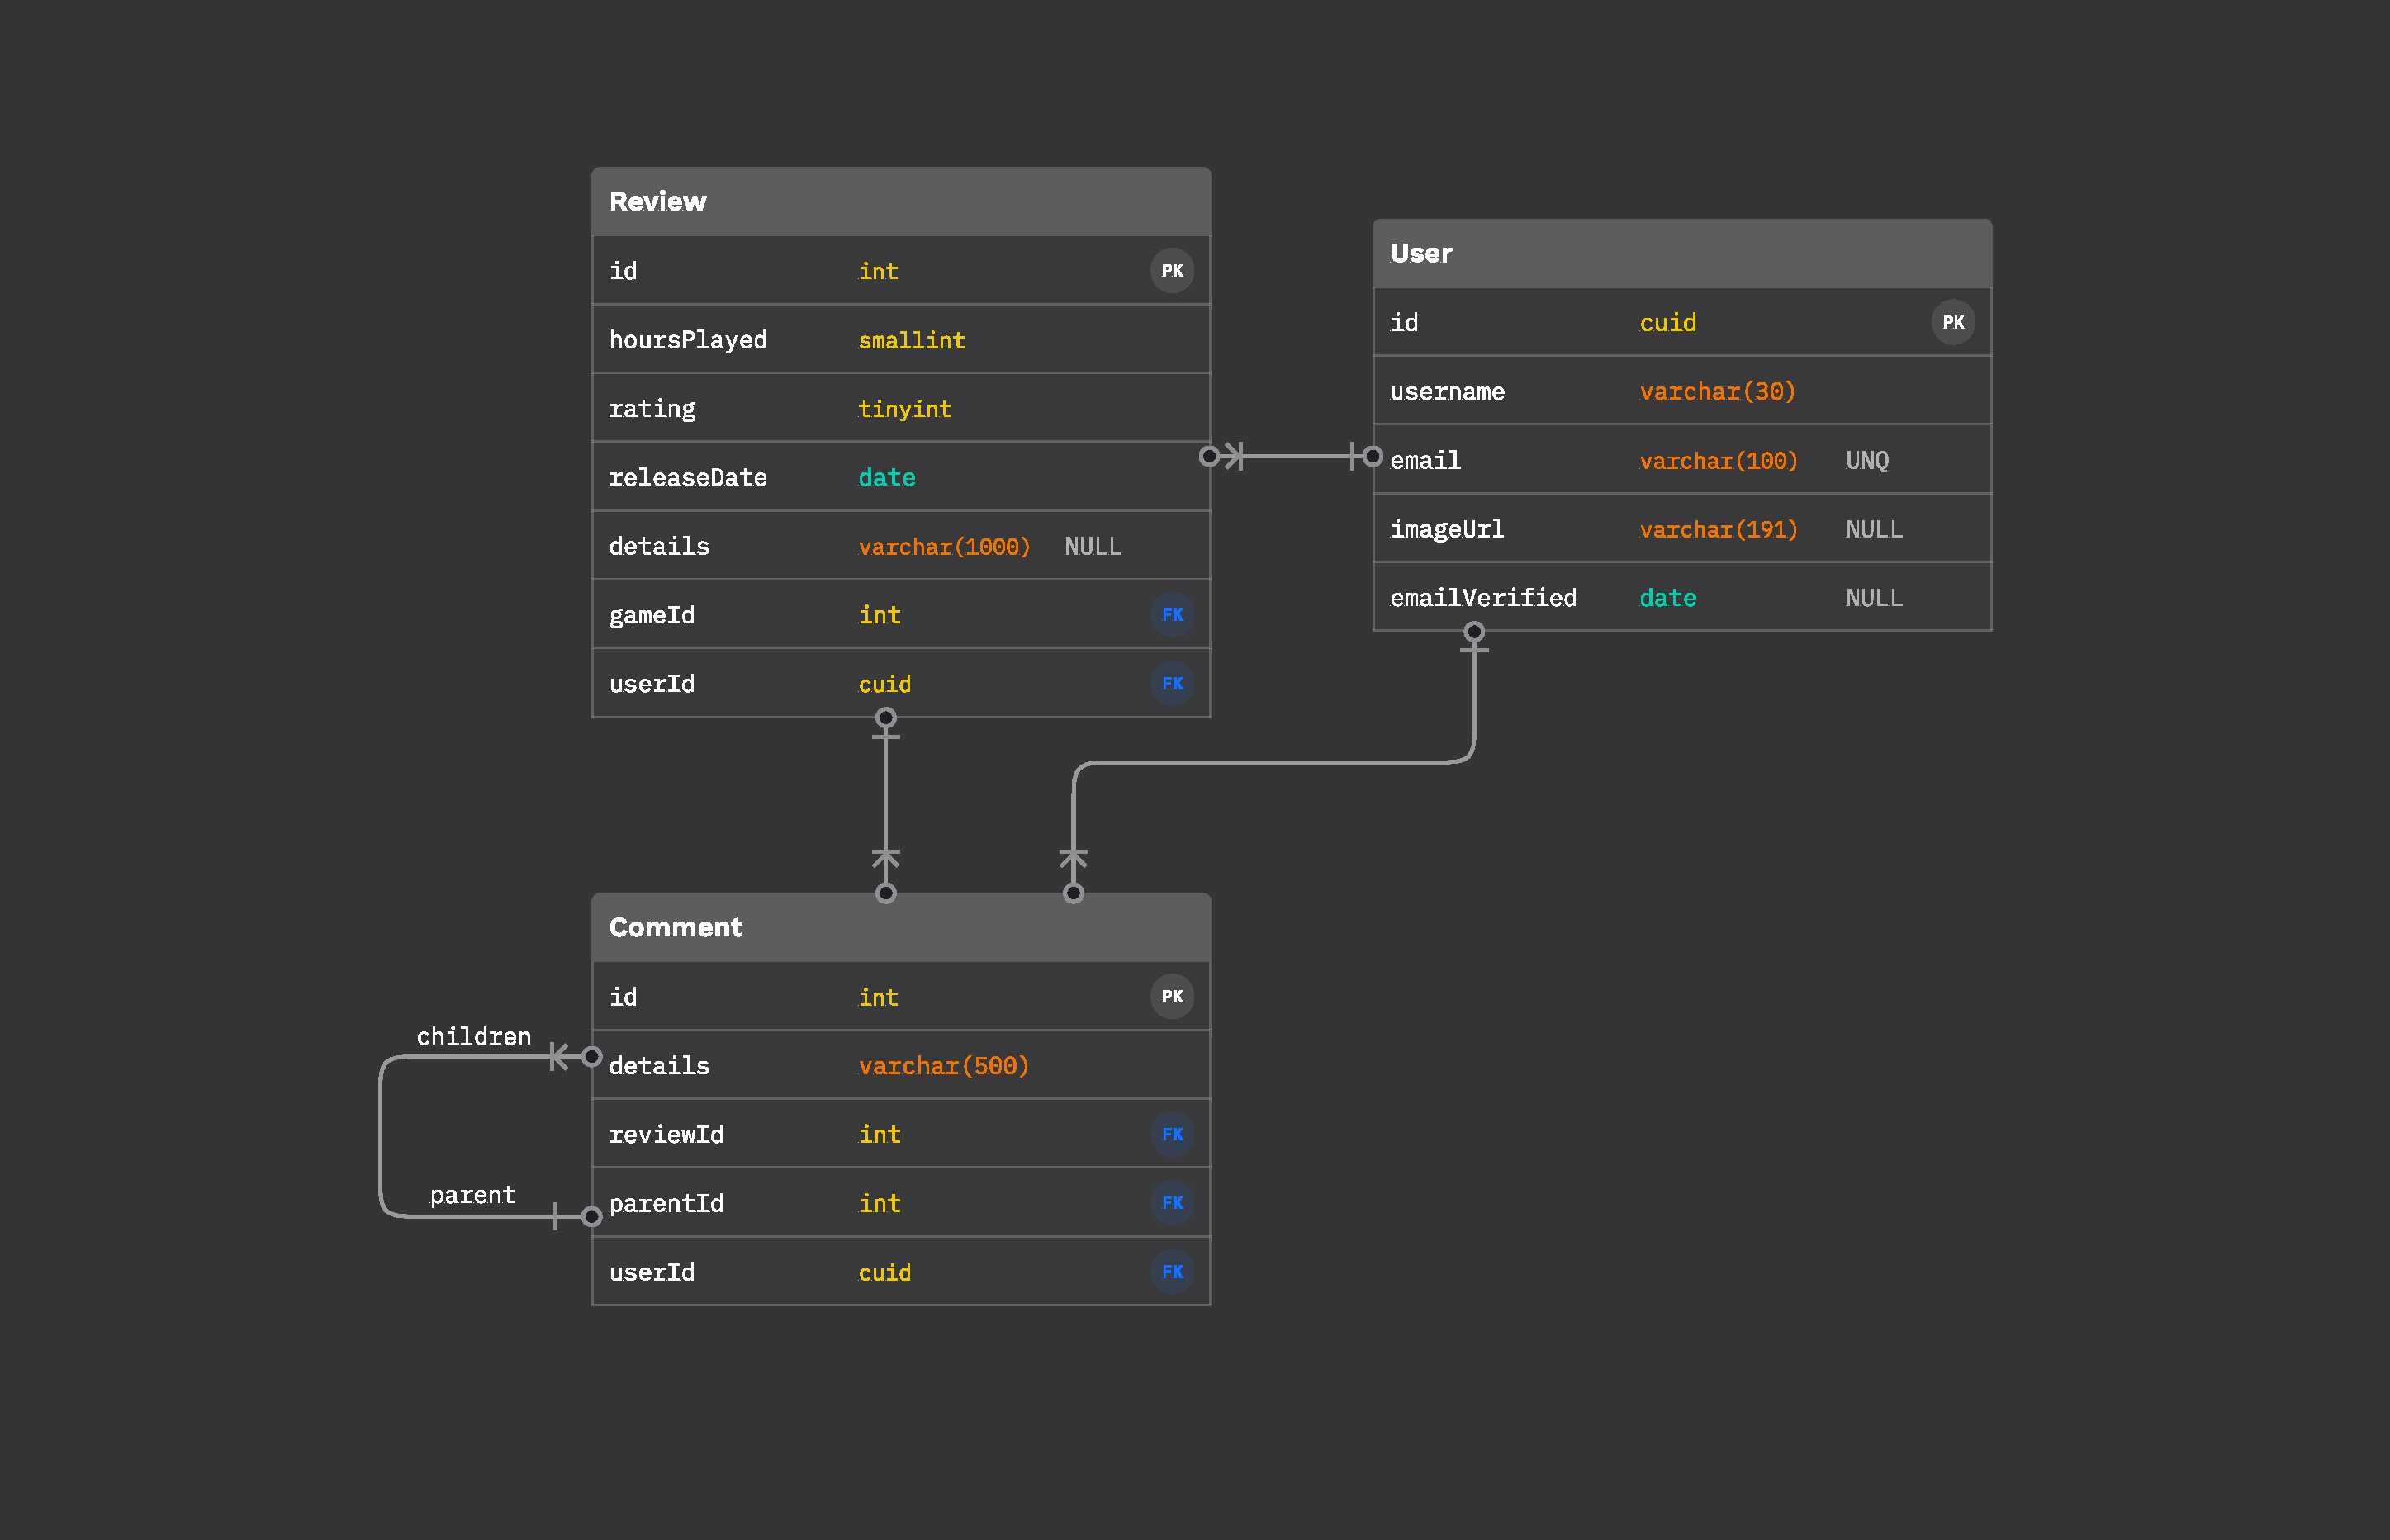
\includegraphics[width=\textwidth]{rdd-comment.pdf}
      \caption{Σχεσιακό διάγραμμα της οντότητας του σχολίου}
    \end{center}
    \label{fig:commentRdd}
  \end{figure}

  Στη περίπτωση της οντότητας της λίστας (\textlatin{Playlist}), η λογική
  της λειτουργικότητας αυτής είναι να δίνει στο χρήστη τη δυνατότητα να
  δημιουργεί λίστες με τα αγαπημένα του βιντεοπαιχνίδια. Ο κάθε χρήστης
  έχει κατά την εγγραφή του στην εφαρμογή πέντε (5) λίστες:
  \begin{itemize}
    \item
      Αγαπημένα (\textlatin{Liked}): Τα βιντεοπαιχνίδια που άρεσαν στον
      χρήστη, η πιο εύχρηστη λίστα για τον χρήστη
    \item
      Λίστα αναμονής (\textlatin{Backlog}): Τα βιντεοπαιχνίδια που θέλει να
      παίξει στο μέλλον
    \item
      Ολοκληρωμένα (\textlatin{Completed}): Τα βιντεοπαιχνίδια που έχει
      παίξει και φτάσει στο τέλος τους στο παρελθόν παίξει στο μέλλον
    \item
      Ενεργά (\textlatin{Playing}): Τα βιντεοπαιχνίδια που παίζει αυτή τη
      χρονική περίοδο
    \item
      Εγκαταλειμμένα (\textlatin{Dropped}): Τα βιντεοπαιχνίδια που δεν του
      άρεσαν και τα έχει εγκαταλείψει
  \end{itemize}

  Ο χρήστης έχει το δικαίωμα να δημιουργήσει όσες ακόμα προσαρμοσμένες
  \textlatin{(Custom)} λίστες θέλει, και να τις μοιραστεί είτε με τους
  ακολούθους του, είτε να τις κάνει δημόσιες, είτε να τις κρατήσει ως
  ιδιωτικές.

  \begin{figure}[H]
    \begin{center}
      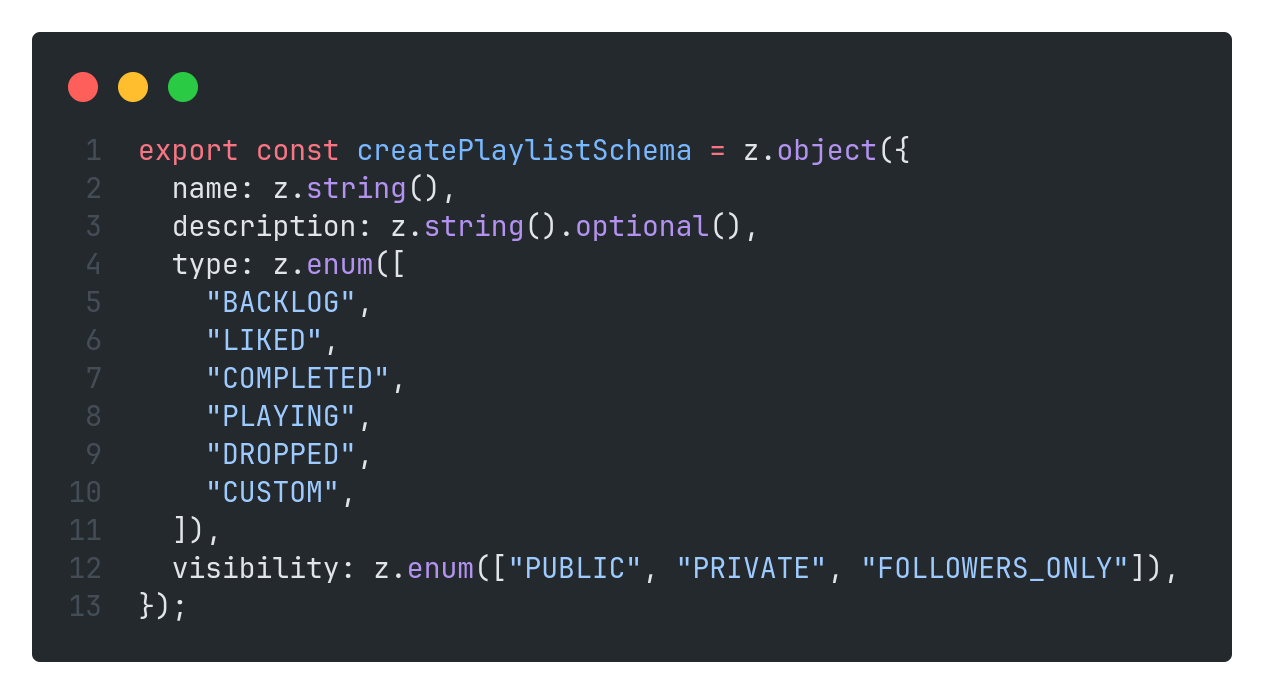
\includegraphics[width=\textwidth]{playlistschema.png}
      \caption{Τύπος δεδομένων για την δημιουργία της οντότητας της
      λίστας}
    \end{center}
    \label{fig:playlistSchema}
  \end{figure}

  Κάθε λίστα έχει μια σχέση 1:Μ με τον χρήστη, μια σχέση 1:Μ με τις
  αντιδράσεις, και μία σχέση Ν:Μ με βιντεοπαιχνίδια. Η σχέση με τα
  βιντεοπαιχνίδια υλοποιείται μέσω ενός πίνακα σύνδεσης
  \cite{AtlassianJoin}, ο οποίος, πέρα από τα ξένα κλειδιά του
  βιντεοπαιχνιδιού και της λίστας, περιέχει και το πεδίο
  \textlatin{order}, το οποίο καθορίζει τη σειρά με την οποία τα
  βιντεοπαιχνίδια εμφανίζονται στη λίστα. Η λογική πίσω από την υλοποίηση
  προϋπόθεται τη χρήση μιας διπλά συνδεμένης λίστας, προκειμένου να
  διατηρείται η επιθυμητή σειρά, αν ο χρήστης αποφασίσει να αλλάξει τη
  σειρά με την οποία τα βιντεοπαιχνίδια θα εμφανίζονται στη λίστα.

  \begin{figure}[H]
    \begin{center}
      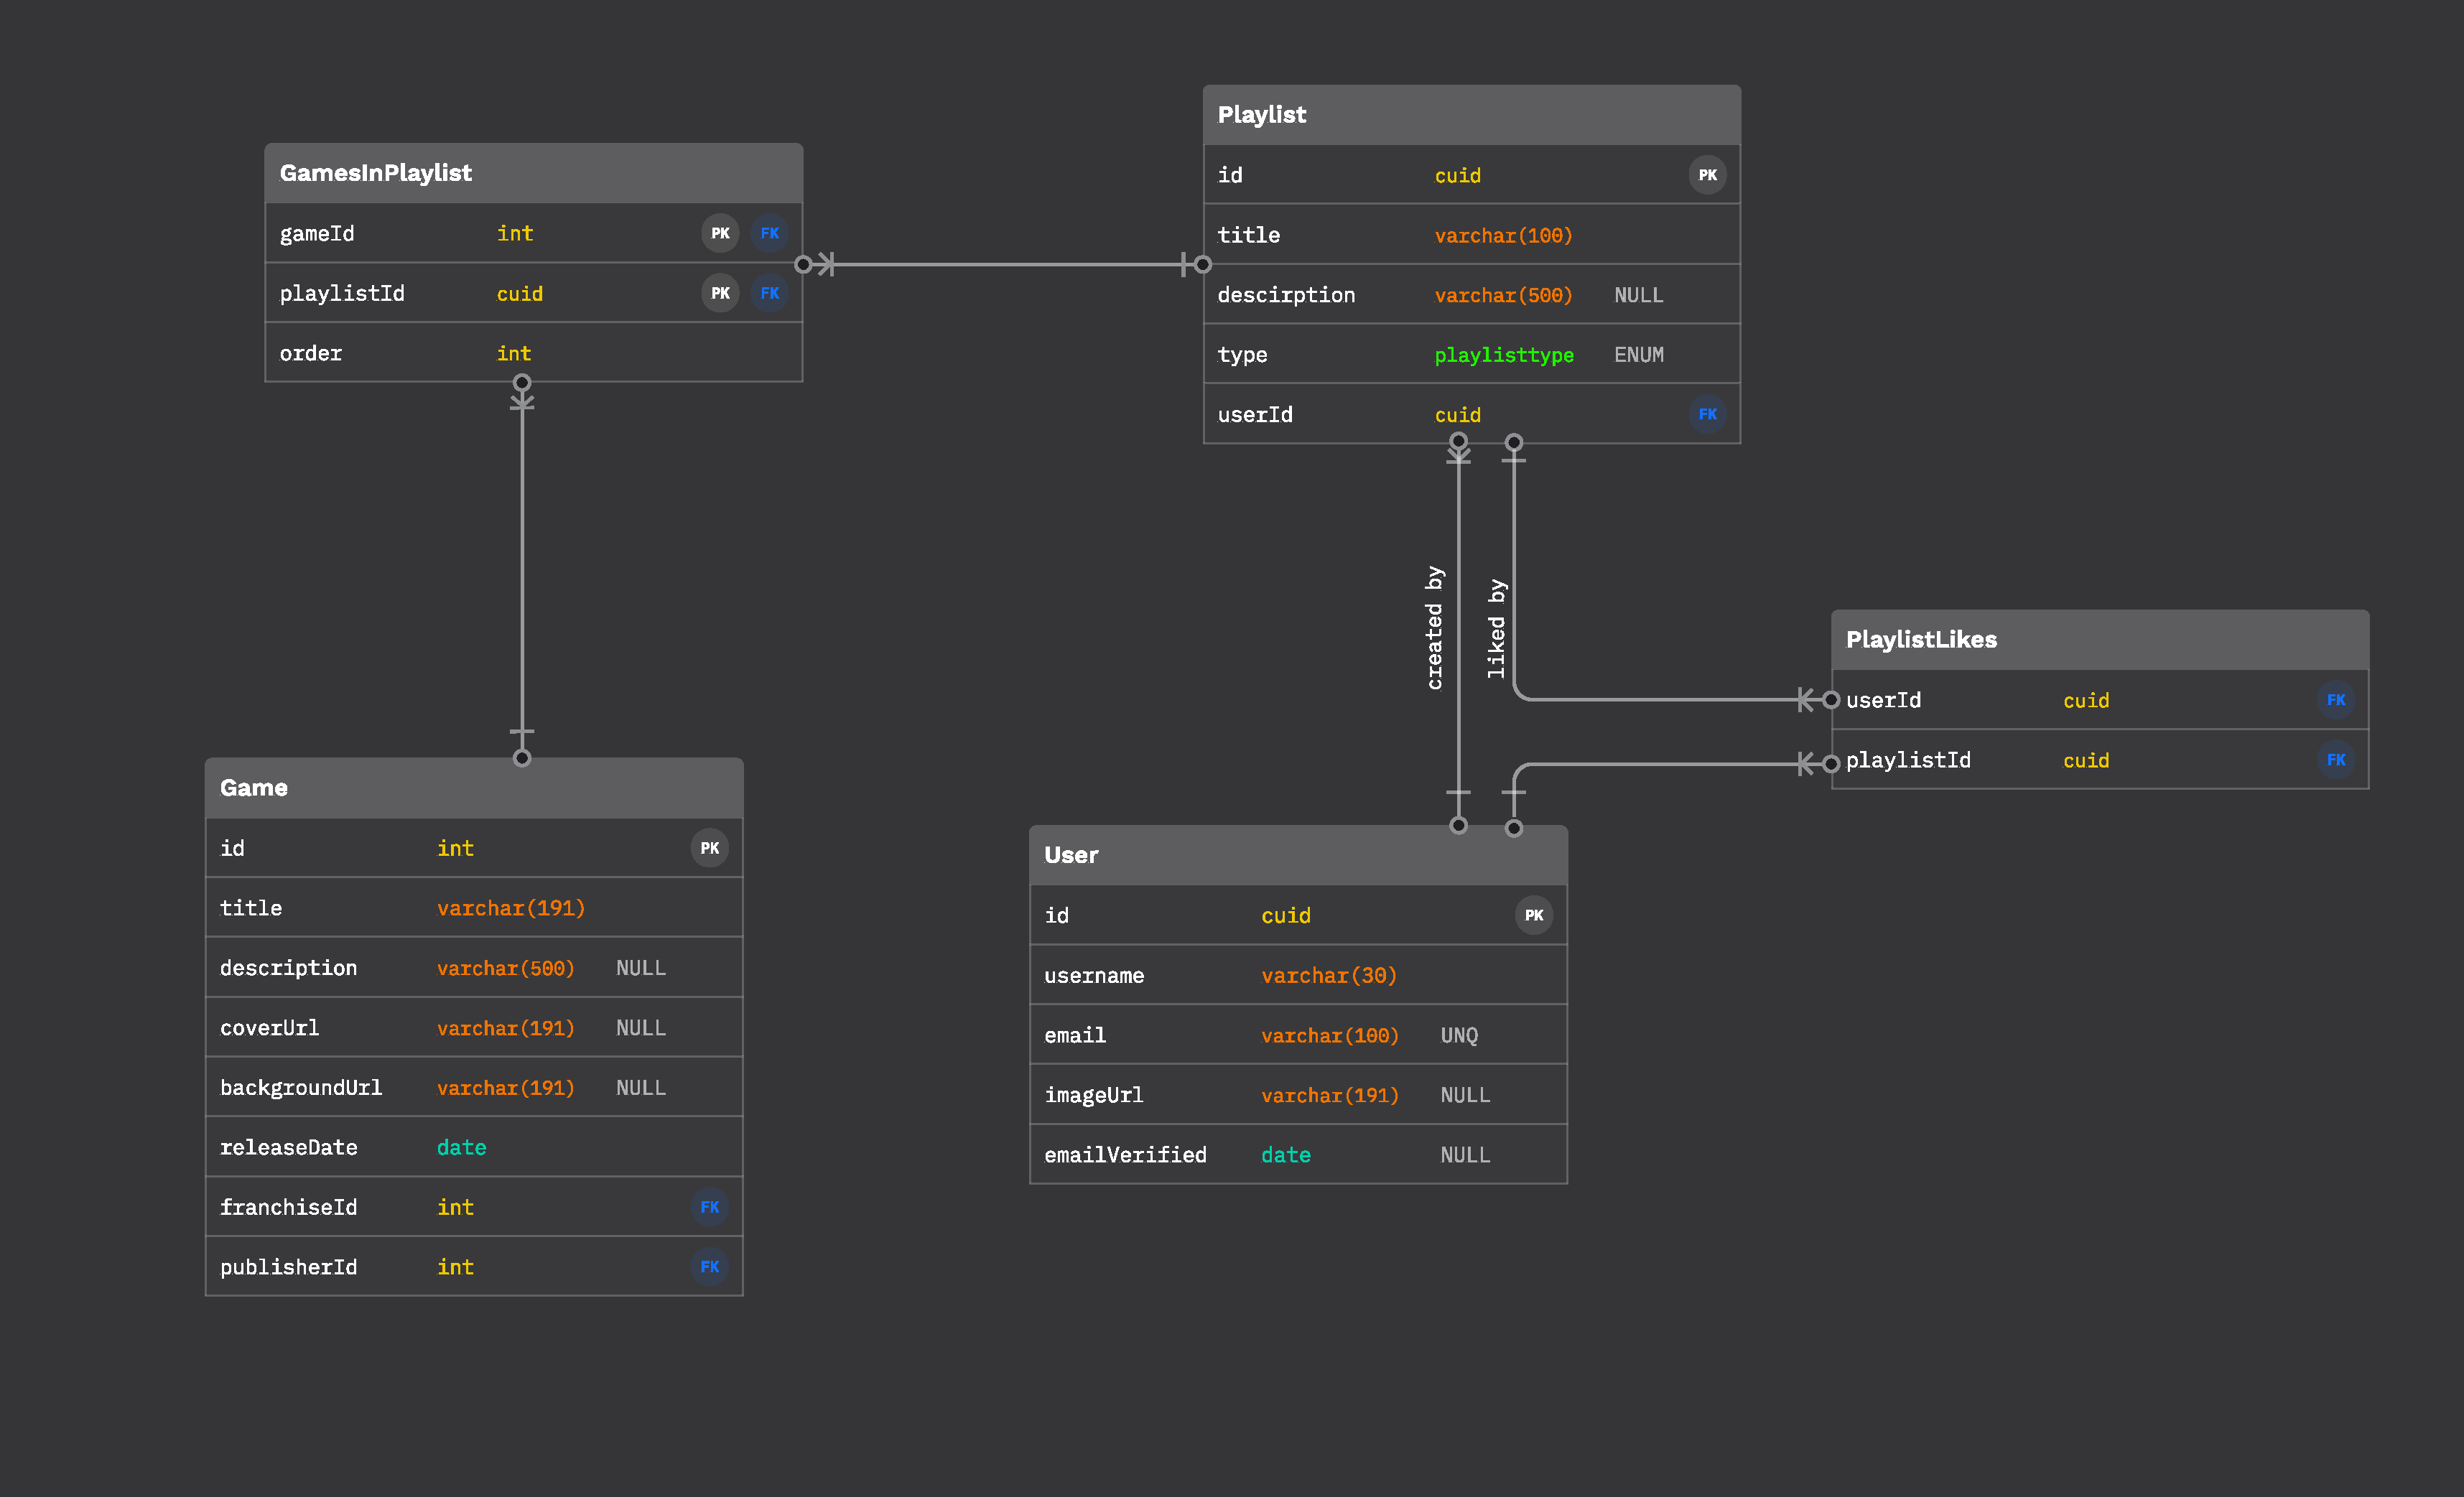
\includegraphics[width=\textwidth]{playlistrdd.pdf}
      \caption{Σχεσιακό διάγραμμα της οντότητας της λίστας}
    \end{center}
    \label{fig:playlistRdd}
  \end{figure}

  Το μοντέλο του \textlatin{GitHub Copilot} αδυνατούσε να ακολουθήσει την
  λογική, με αποτέλεσμα να χρειαστεί να υλοποιηθούν εξ᾽ ολοκλήρου από τον
  προγραμματιστή.

  \begin{figure}[H]
    \begin{center}
      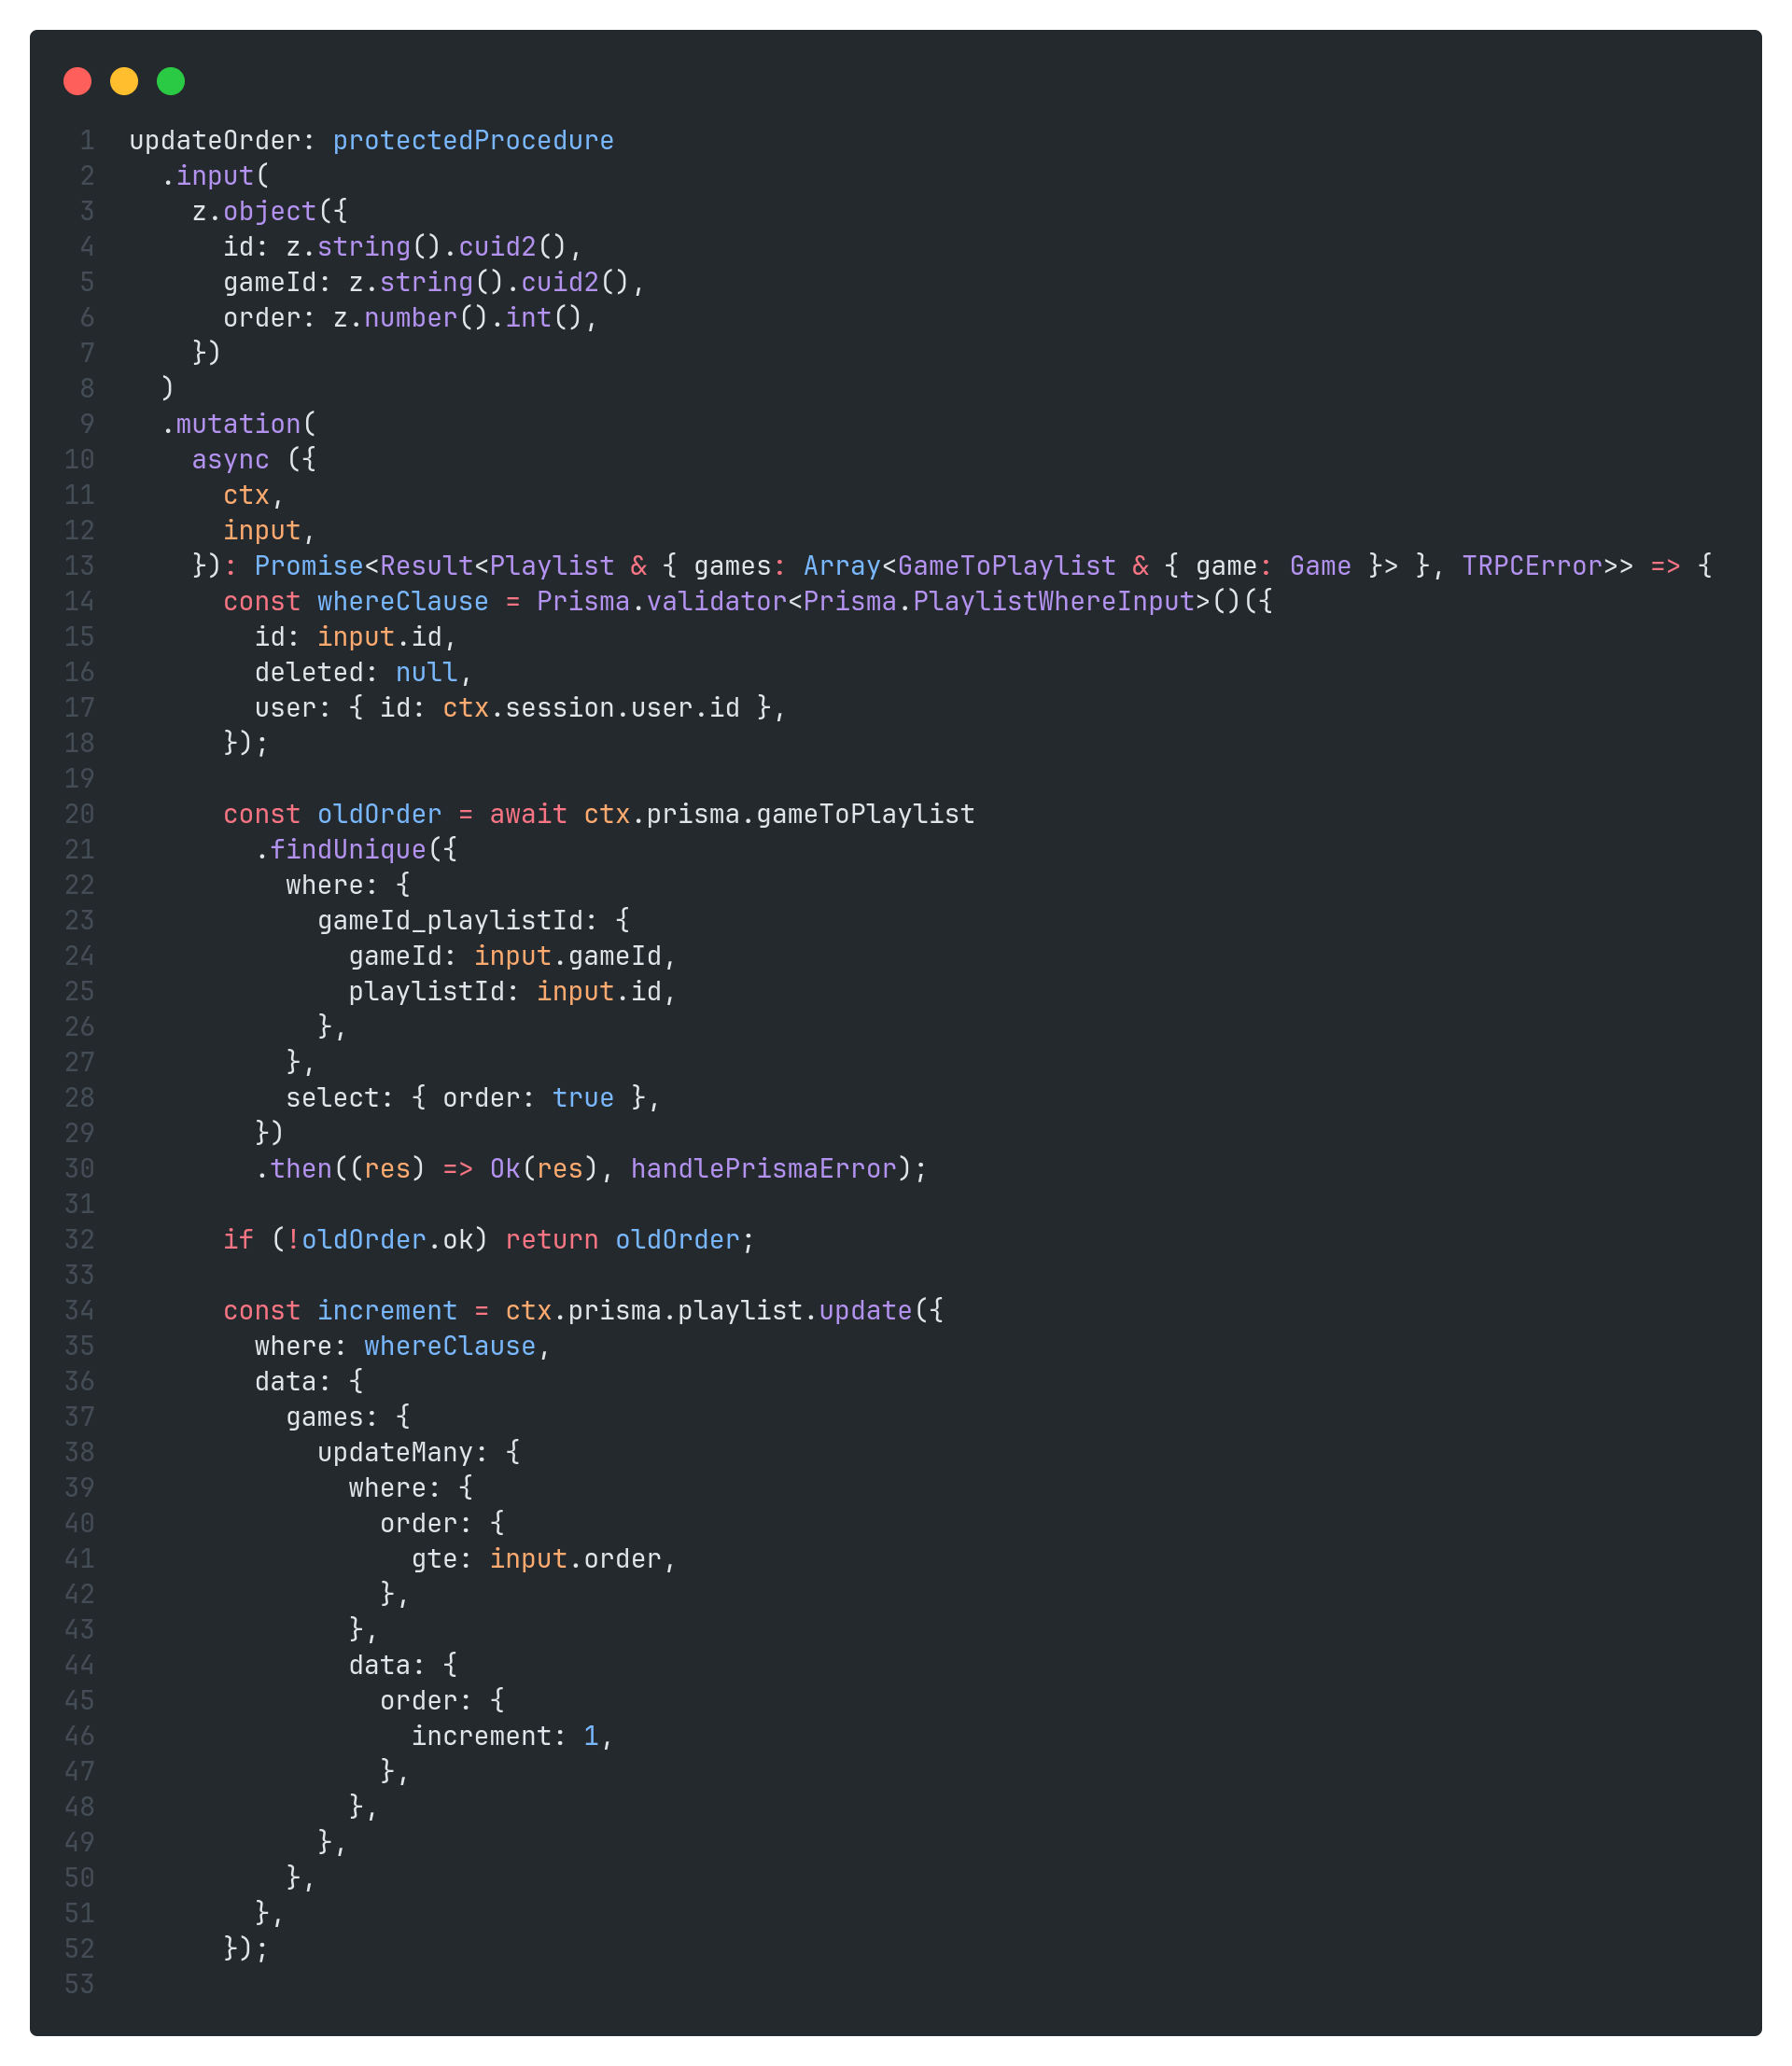
\includegraphics[width=\textwidth]{updateorder.png}
      \caption{Παράδειγμα μεθόδου που αφορά την αλλαγή της σειράς των
      βιντεοπαιχνιδιών στη λίστα, \textit{Μέρος 1}}
    \end{center}
    \label{fig:updateOrder}
  \end{figure}

  \begin{figure}[H]
    \begin{center}
      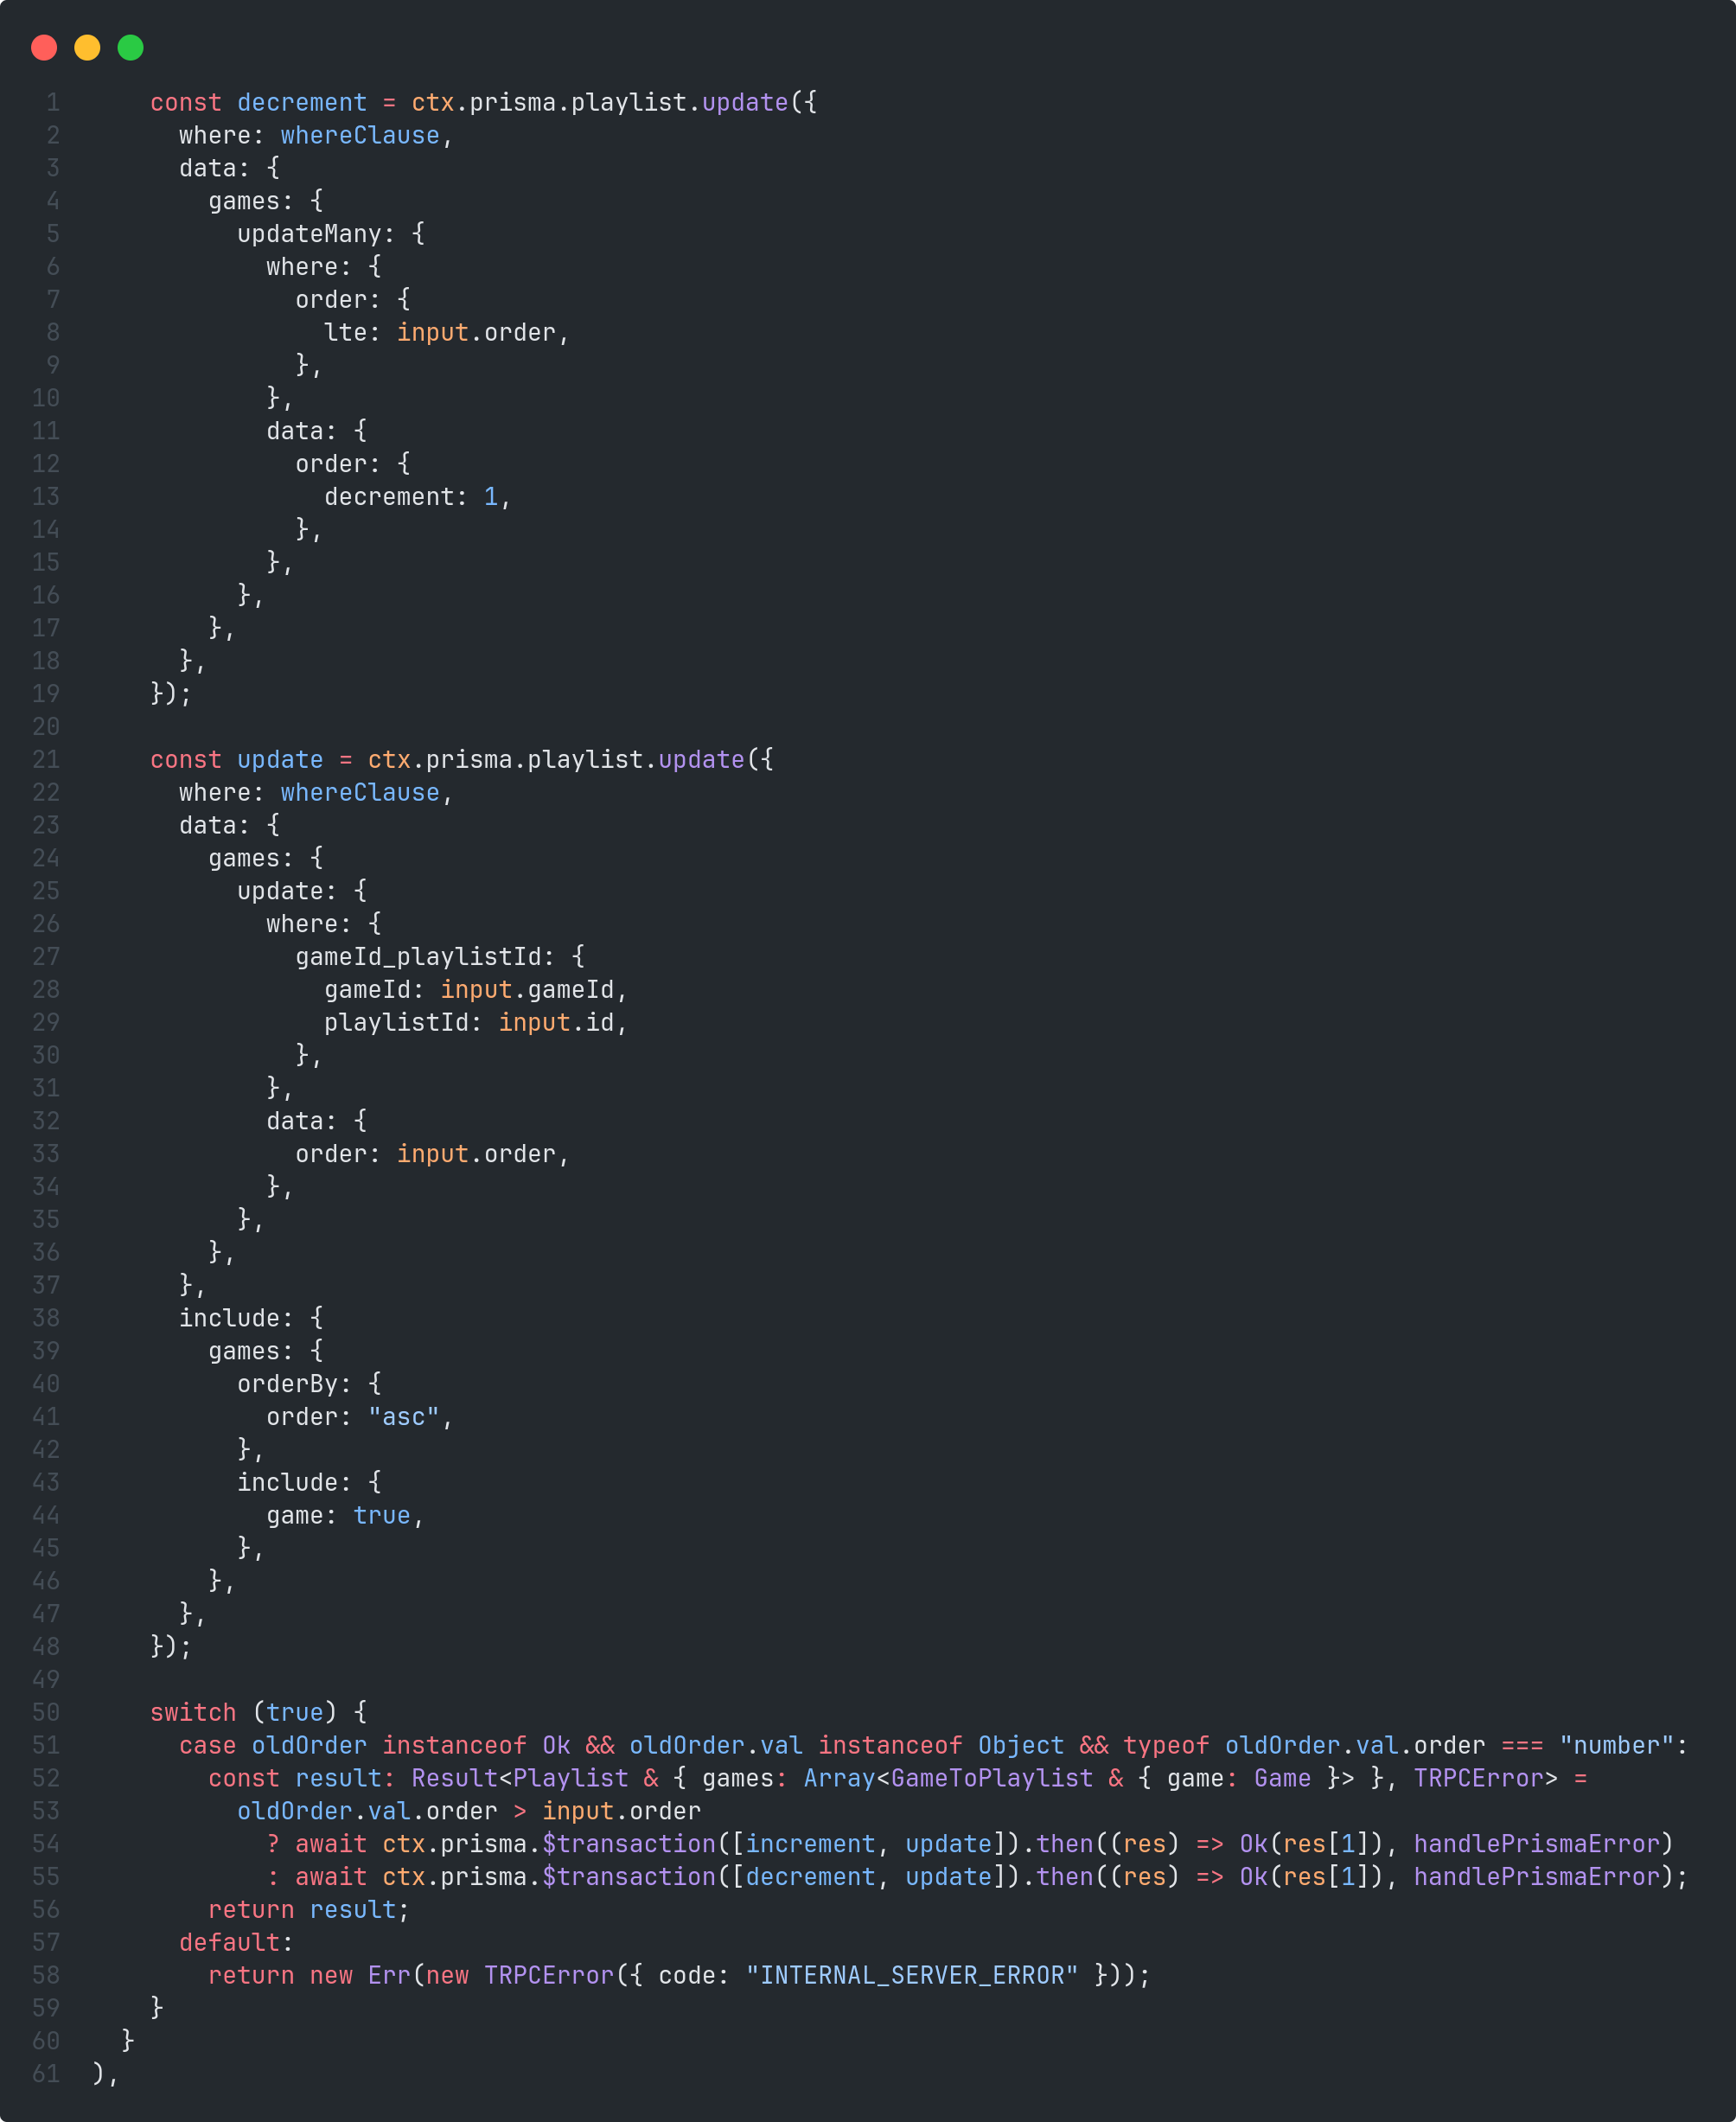
\includegraphics[width=\textwidth]{updateorder2.png}
      \caption{Παράδειγμα μεθόδου που αφορά την αλλαγή της σειράς των
      βιντεοπαιχνιδιών στη λίστα, \textit{Μέρος 2}}
    \end{center}
    \label{fig:updateOrder2}
  \end{figure}

  Πέρα από τη σειρά των βιντεοπαιχνιδιών, σημαντική ήταν και η εξασφάλιση
  της ορθής ορατότητας της λίστας σε άλλους χρήστες, χωρίς να επιτρέπεται
  η πρόσβαση σε λίστες που δεν είναι είτε δημόσιες, είτε ανήκουν σε
  χρήστες που ο χρήστης ακολουθεί, είτε είναι προσωπικές λίστες του ίδιου.
  Στην περίπτωση αυτή, αν και το μοντέλο ακολούθησε τη σωστή λογική,
  αδυνάτισε να βρει το σωστό ερώτημα προς τη βάση όσο αφορά την ορατότητα
  της λίστας προς τους ακολούθους του χρήστη.

  \begin{figure}[H]
    \begin{center}
      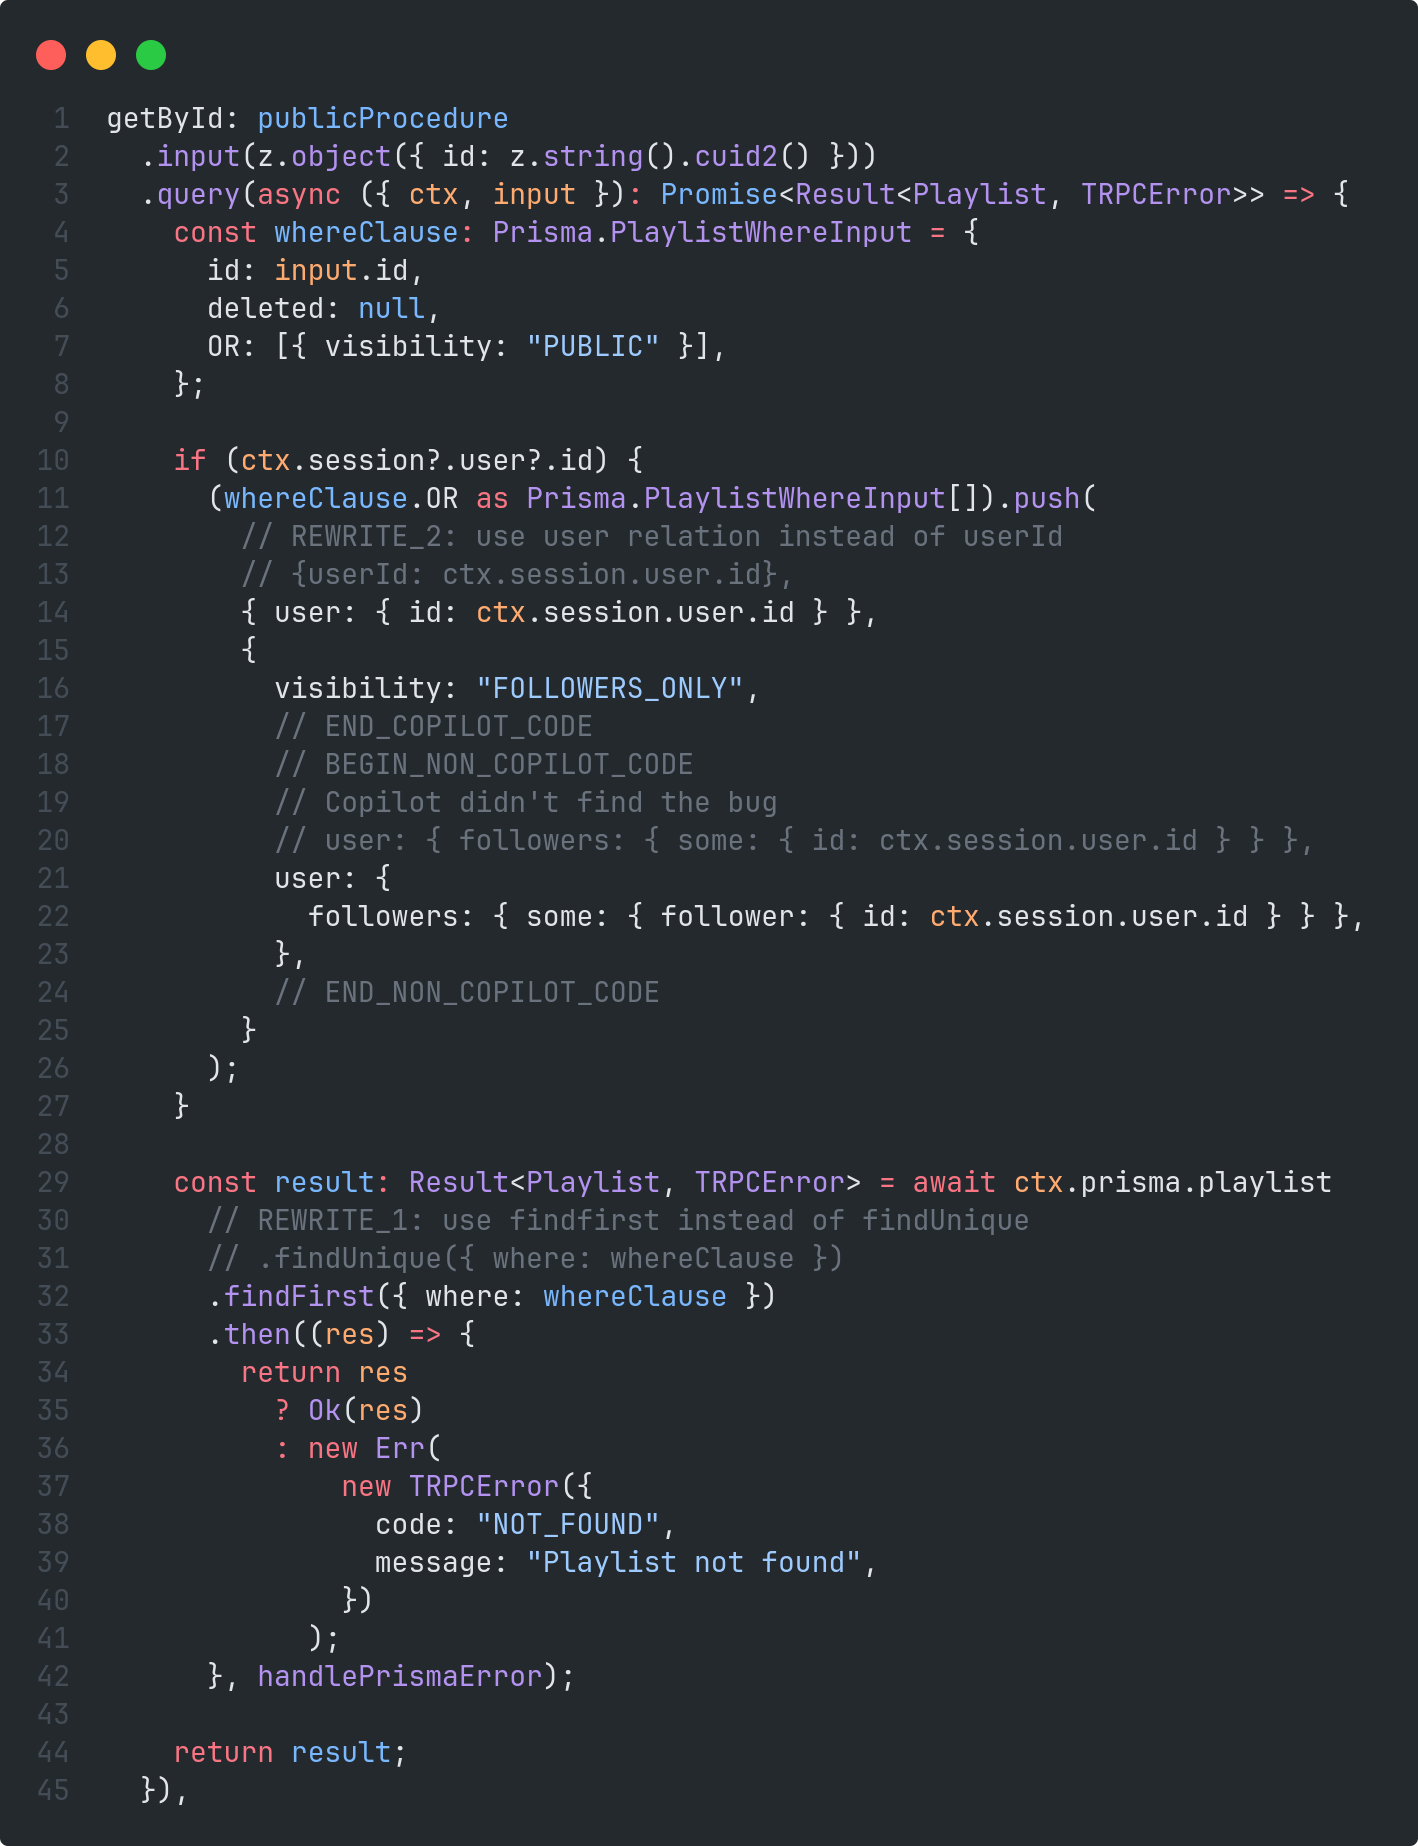
\includegraphics[width=\textwidth]{getbyidplaylist.png}
      \caption{Παράδειγμα μεθόδου που αφορά την ανάκτηση λίστας με βάση το
      αναγνωριστικό της}
    \end{center}
    \label{fig:getByIdPlaylist}
  \end{figure}

  Όπως παρατηρείται στο διάγραμμα \ref{fig:getByIdPlaylist}, το μοντέλο
  ορθά αναγνώρισε ότι σε περίπτωση που μια λίστα δημοσιεύονταν μόνο στους
  ακολούθους του δημιουργού της, θα έπρεπε ο χρήστης που την ανακτά θα
  έπρεπε να ανήκει στην λίστα των ακολούθων του δημιουργού, η υλοποίηση
  του κώδικα δεν ήταν σωστή, καθώς αγνόησε την Μ:Ν σχέση μεταξύ των
  χρηστών και των ακολούθων τους.

  \begin{figure}[H]
    \begin{center}
      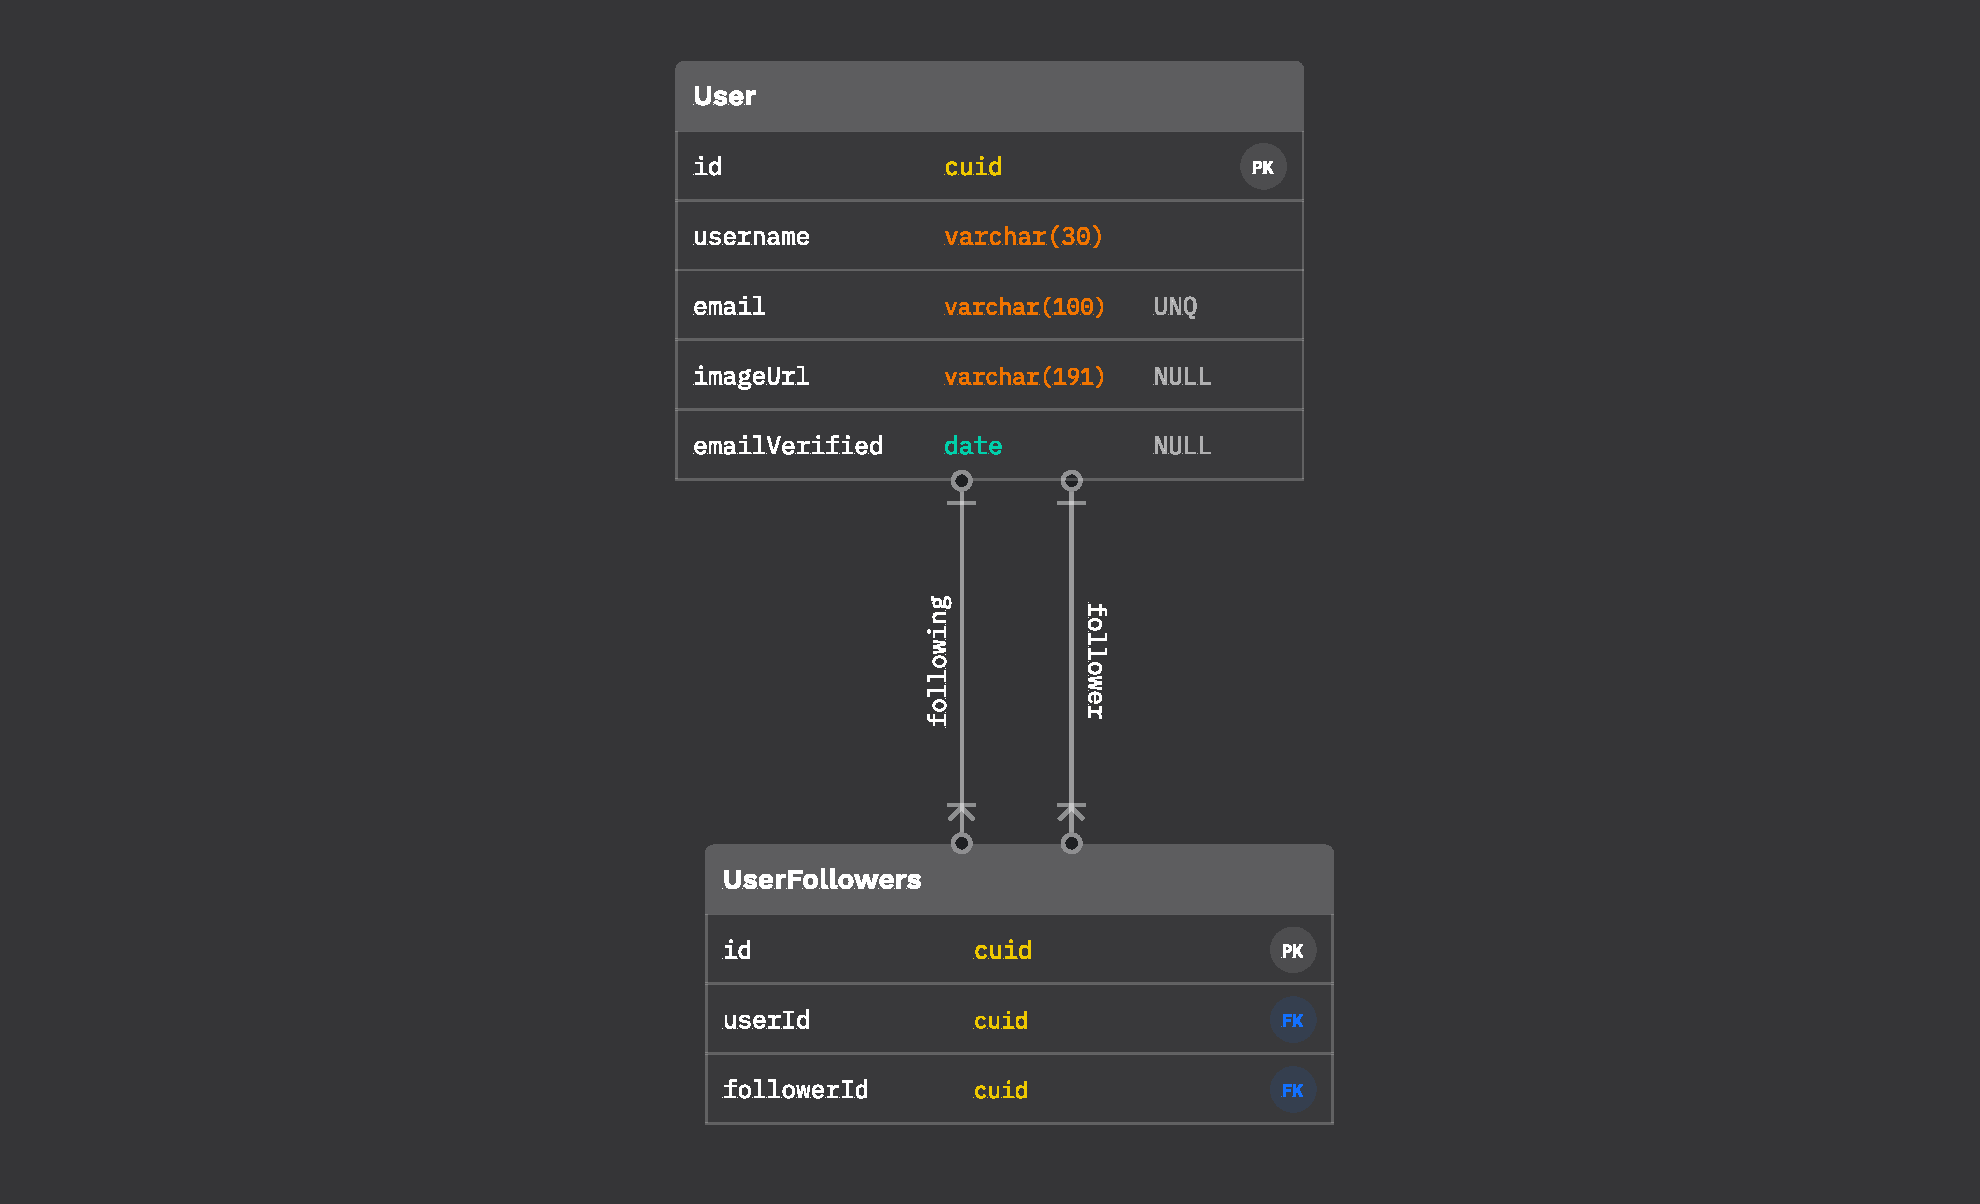
\includegraphics[width=\textwidth]{userfollower.pdf}
      \caption{Σχεσιακό διάγραμμα της σχέσης μεταξύ χρηστών και ακολούθων}
    \end{center}
    \label{fig:userFollower}
  \end{figure}

  Στις περιπτώσεις των αρχείων που αφορούσαν το \textlatin{Integration
  Testing}, οι αλλαγές ήταν οι περίσσοτερες συγκριτικά με τις
  περιπτώσεις ανάπτυξης του \textlatin{API} και του \textlatin{Unit
  Testing} και οι αλλαγές από την πλευρά του μοντέλου ήταν αρκετά πιο
  ισορροπημένες, με τις αλλαγές σε μεγάλη έκταση κώδικα να υπερβαίνουν
  αυτών της μικρής έκτασης κώδικα.

  Στην περίπτωση αυτή, ρόλο έπαιξε το γεγονός ότι κατά την γραφή των
  ελέγχων, το εργαλείο \textlatin{Jest}, παρέχει τη δυνατότητα στον
  προγραμματιστή να συντάξει μια περιγραφή για τον έλεγχο, μέσω των
  μεθόδων \textit{\textlatin{describe}} και \textit{\textlatin{it}}. Οι
  μέθοδοι αυτές, παίρνουν ως πρώτο όρισμα μια συμβολοσειρά που περιγράφει
  τον έλεγχο, και ως δεύτερο όρισμα μια συνάρτηση \textlatin{callback}
  \cite{crockfordjavascript} που περιέχει τον κώδικα του ελέγχου. Η
  περιγραφή του ελέγχου, ακολουθεί την ανάπτυξη \textbf{Λογισμικού
  Καθοδηγούμενη Από Τη Συμπεριφορά} (\textlatin{Behavior Driven
  Development, BDD}).

  Η \textlatin{BDD} είναι μια προσέγγιση στην ανάπτυξη λογισμικού που
  επικεντρώνεται στη συμπεριφορά του συστήματος από την οπτική γωνία του
  χρήστη. Ενθαρρύνει τη συνεργασία μεταξύ προγραμματιστών, ελεγκτών και μη
  τεχνικών ενδιαφερομένων, χρησιμοποιώντας μια κοινή γλώσσα για να
  περιγράψει την επιθυμητή συμπεριφορά του λογισμικού. Συνήθως
  περιλαμβάνει τη συγγραφή σεναρίων ή παραδειγμάτων που περιγράφουν πώς το
  λογισμικό θα πρέπει να συμπεριφέρεται σε διάφορες καταστάσεις, συχνά
  χρησιμοποιώντας τη μορφή \say{Δεδομένου-Όταν-Τότε}
  (\say{\textlatin{Given-When-Then}}). Αυτά τα σενάρια λειτουργούν τόσο ως
  προδιαγραφές όσο και ως περιπτώσεις δοκιμών, βοηθώντας να διασφαλιστεί
  ότι το αναπτυγμένο λογισμικό ανταποκρίνεται στις προβλεπόμενες
  απαιτήσεις και συμπεριφέρεται σωστά από την οπτική γωνία του χρήστη.
  \cite{bddstudy,mughal2024advancingbddsoftwaretesting,bddsystematic}

  \begin{figure}[H]
    \begin{center}
      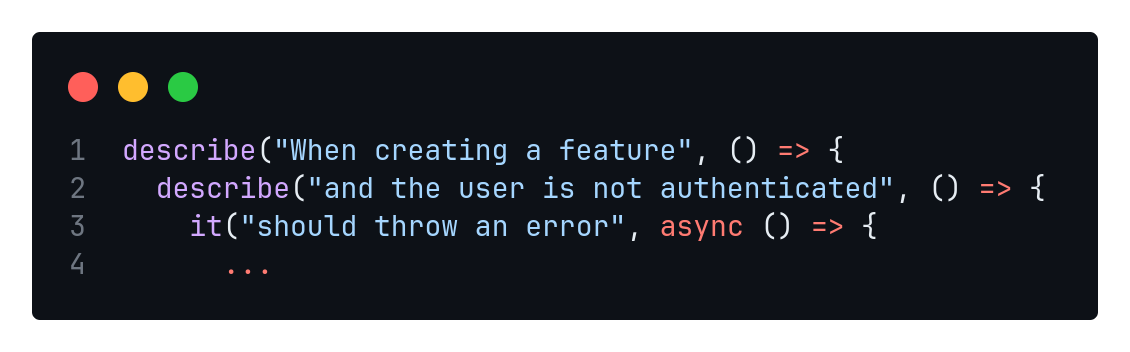
\includegraphics[width=\textwidth]{test_general.png}
      \caption{Παράδειγμα μεθόδου που αφορά την δημιουργία ενός ελέγχου,
        με χρήση των μεθόδων \textit{\textlatin{describe}} και
      \textit{\textlatin{it}}}
    \end{center}
    \label{fig:TestGeneral}
  \end{figure}

  \begin{figure}[H]
    \begin{center}
      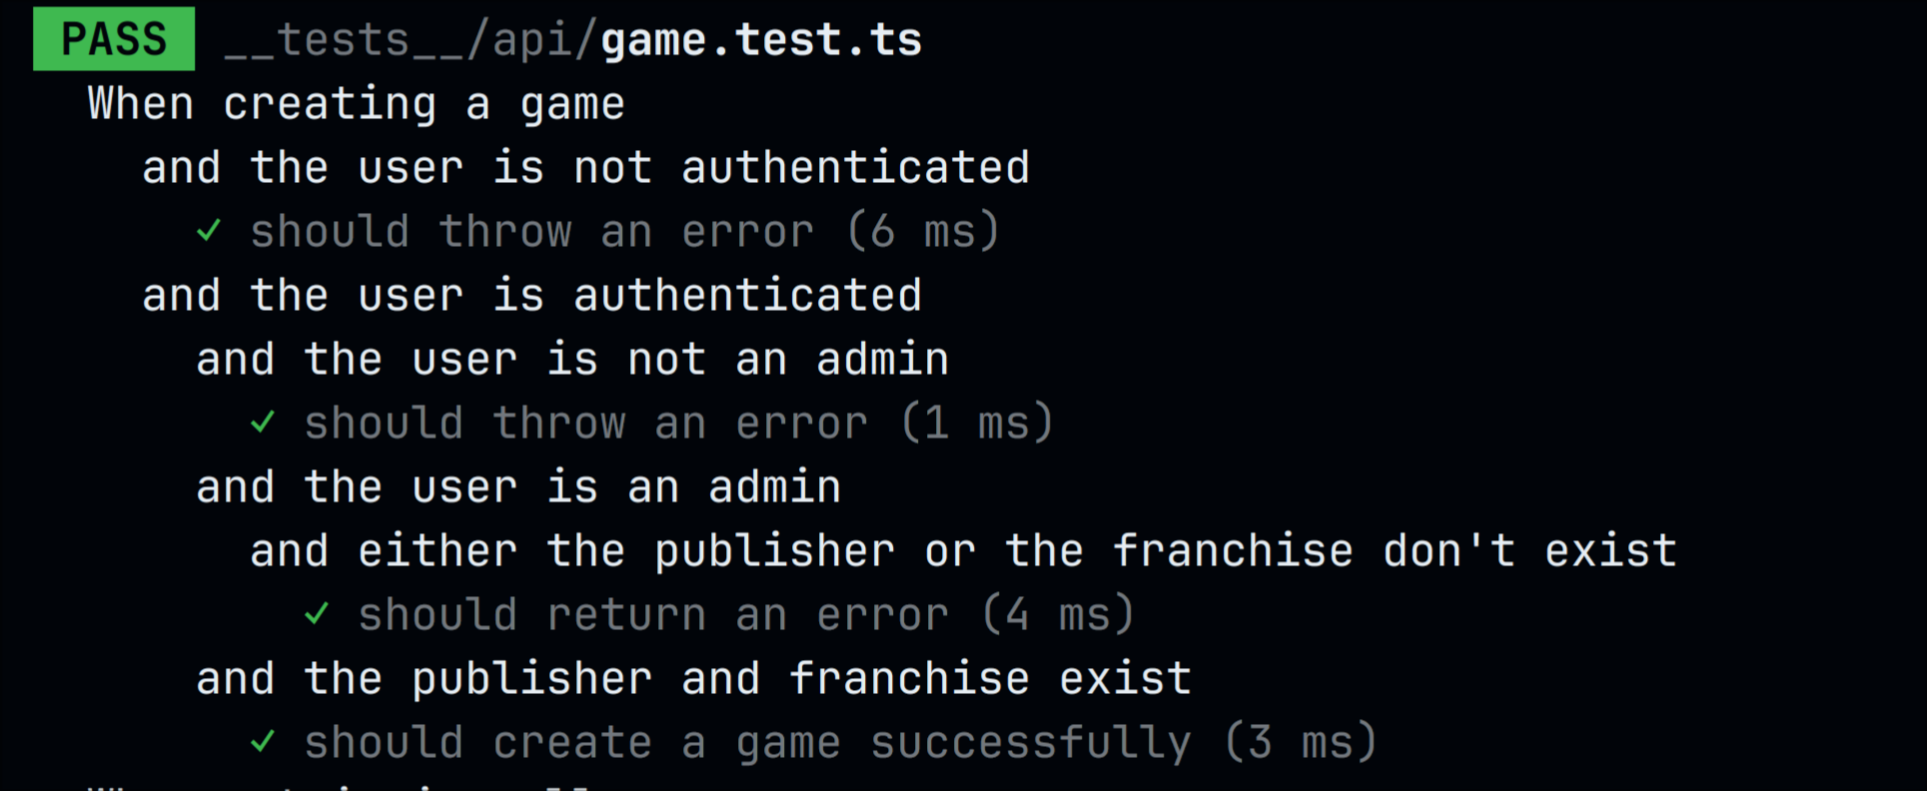
\includegraphics[width=\textwidth]{test_terminal.png}
      \caption{Παράδειγμα αποτελέσματος ελέγχου σε διεπαφή τερματικού, με
        χρήση των μεθόδων \textit{\textlatin{describe}} και
      \textit{\textlatin{it}}, μέσω του εργαλείου \textlatin{Jest}}
    \end{center}
    \label{fig:TestGeneralTerminal}
  \end{figure}

  Επειδή το μοντέλο δουλεύει με \textlatin{next token prediction}, και
  έλεγχοι γράφονται ο ένας μετά τον άλλο, το μοντέλο κατά τη συγγραφή των
  ελέγχων, λόγω των περιγραφών που περιέχονται στις μεθόδους, προσπαθούσε
  να γράψει τον έλεγχο με βάση την περιγραφή, αντί του κώδικα της μεθόδου,
  με αποτέλεσμα να οδηγείται συχνά σε λάθη και ανακρίβειες. Αξιοσημείωτη
  είναι η προσθήκη της δυνατότητας του \textlatin{GitHub Copilot Chat} να
  γράψει ελέγχους για μια μέθοδο μέσω μιας εντολής στο πλαίσιο προτροπής
  με το μοντέλο \cite{copilotchattips} τον Μάρτιο του 2024, ωστόσο κατά
  την διάρκεια της δοκιμής του μοντέλου, η συγκεκριμένη δυνατότητα δεν
  ήταν διαθέσιμη.

  Για την διαφορά μεταξύ αναγκαίων αλλαγών στις περιπτώσεις των αρχείων
  που αφορούσαν το \textlatin{Unit Testing} και το \textlatin{Integration
  Testing}, συνέβαλε και το γεγονός στην περίπτωση των ελέγχων μονάδας,
  οι έλεγχοι που πραγματοποιούνται είναι πιο απλοί και πολλές φορές
  χρησιμοποιούνται τεχνικές εικονικής αναπαράστασης εξαρτήσεων, γνωστές
  και ως τεχνικές προσομοίωσης εξαρτήσεων (\textlatin{dependency
  mocking}). Η προσομοίωση εξαρτήσεων είναι μια τεχνική που
  χρησιμοποιείται στους ελέγχους λογισμικού, όπου δημιουγούνται ψεύτικα ή
  προσομοιωμένα αντικείμενα που μιμούνται τη συμπεριφορά πραγματικών
  εξαρτήσεων ενός συστήματος. Αυτό επιτρέπει στους προγραμματιστές να
  ελέγχουν μια μονάδα κώδικα σε απομόνωση, χωρίς να επηρεάζονται από
  εξωτερικές εξαρτήσεις όπως βάσεις δεδομένων, υπηρεσίες δικτύου ή
  πολύπλοκες βιβλιοθήκες. Η προσομοίωση εξαρτήσεων βοηθά στη δημιουργία
  πιο ελεγχόμενων και προβλέψιμων συνθηκών δοκιμής, επιτρέποντας τον
  έλεγχο διαφόρων σεναρίων και καταστάσεων σφάλματος που μπορεί να είναι
  δύσκολο να αναπαραχθούν με πραγματικές εξαρτήσεις
  \cite{freeman2009growing}. Αντίθετα, στην περίπτωση των ελέγχων
  ενσωμάτωσης, οι εξαρτήσεις είναι πραγματικές, και οι ελέγχοι που
  πραγματοποιούνται είναι πιο πολύπλοκοι και απαιτούν την ύπαρξη
  πραγματικών εξαρτήσεων, και χρειάζονται περισσότερη σκέψη για την
  υλοποίησή τους. Παρατίθενται δύο παραδείγματα ελέγχων, ένα από την
  περίπτωση των ελέγχων μονάδας και ένα από την περίπτωση των ελέγχων
  ενσωμάτωσης, για τον ίδιο έλεγχο.

  \begin{figure}[H]
    \begin{center}
      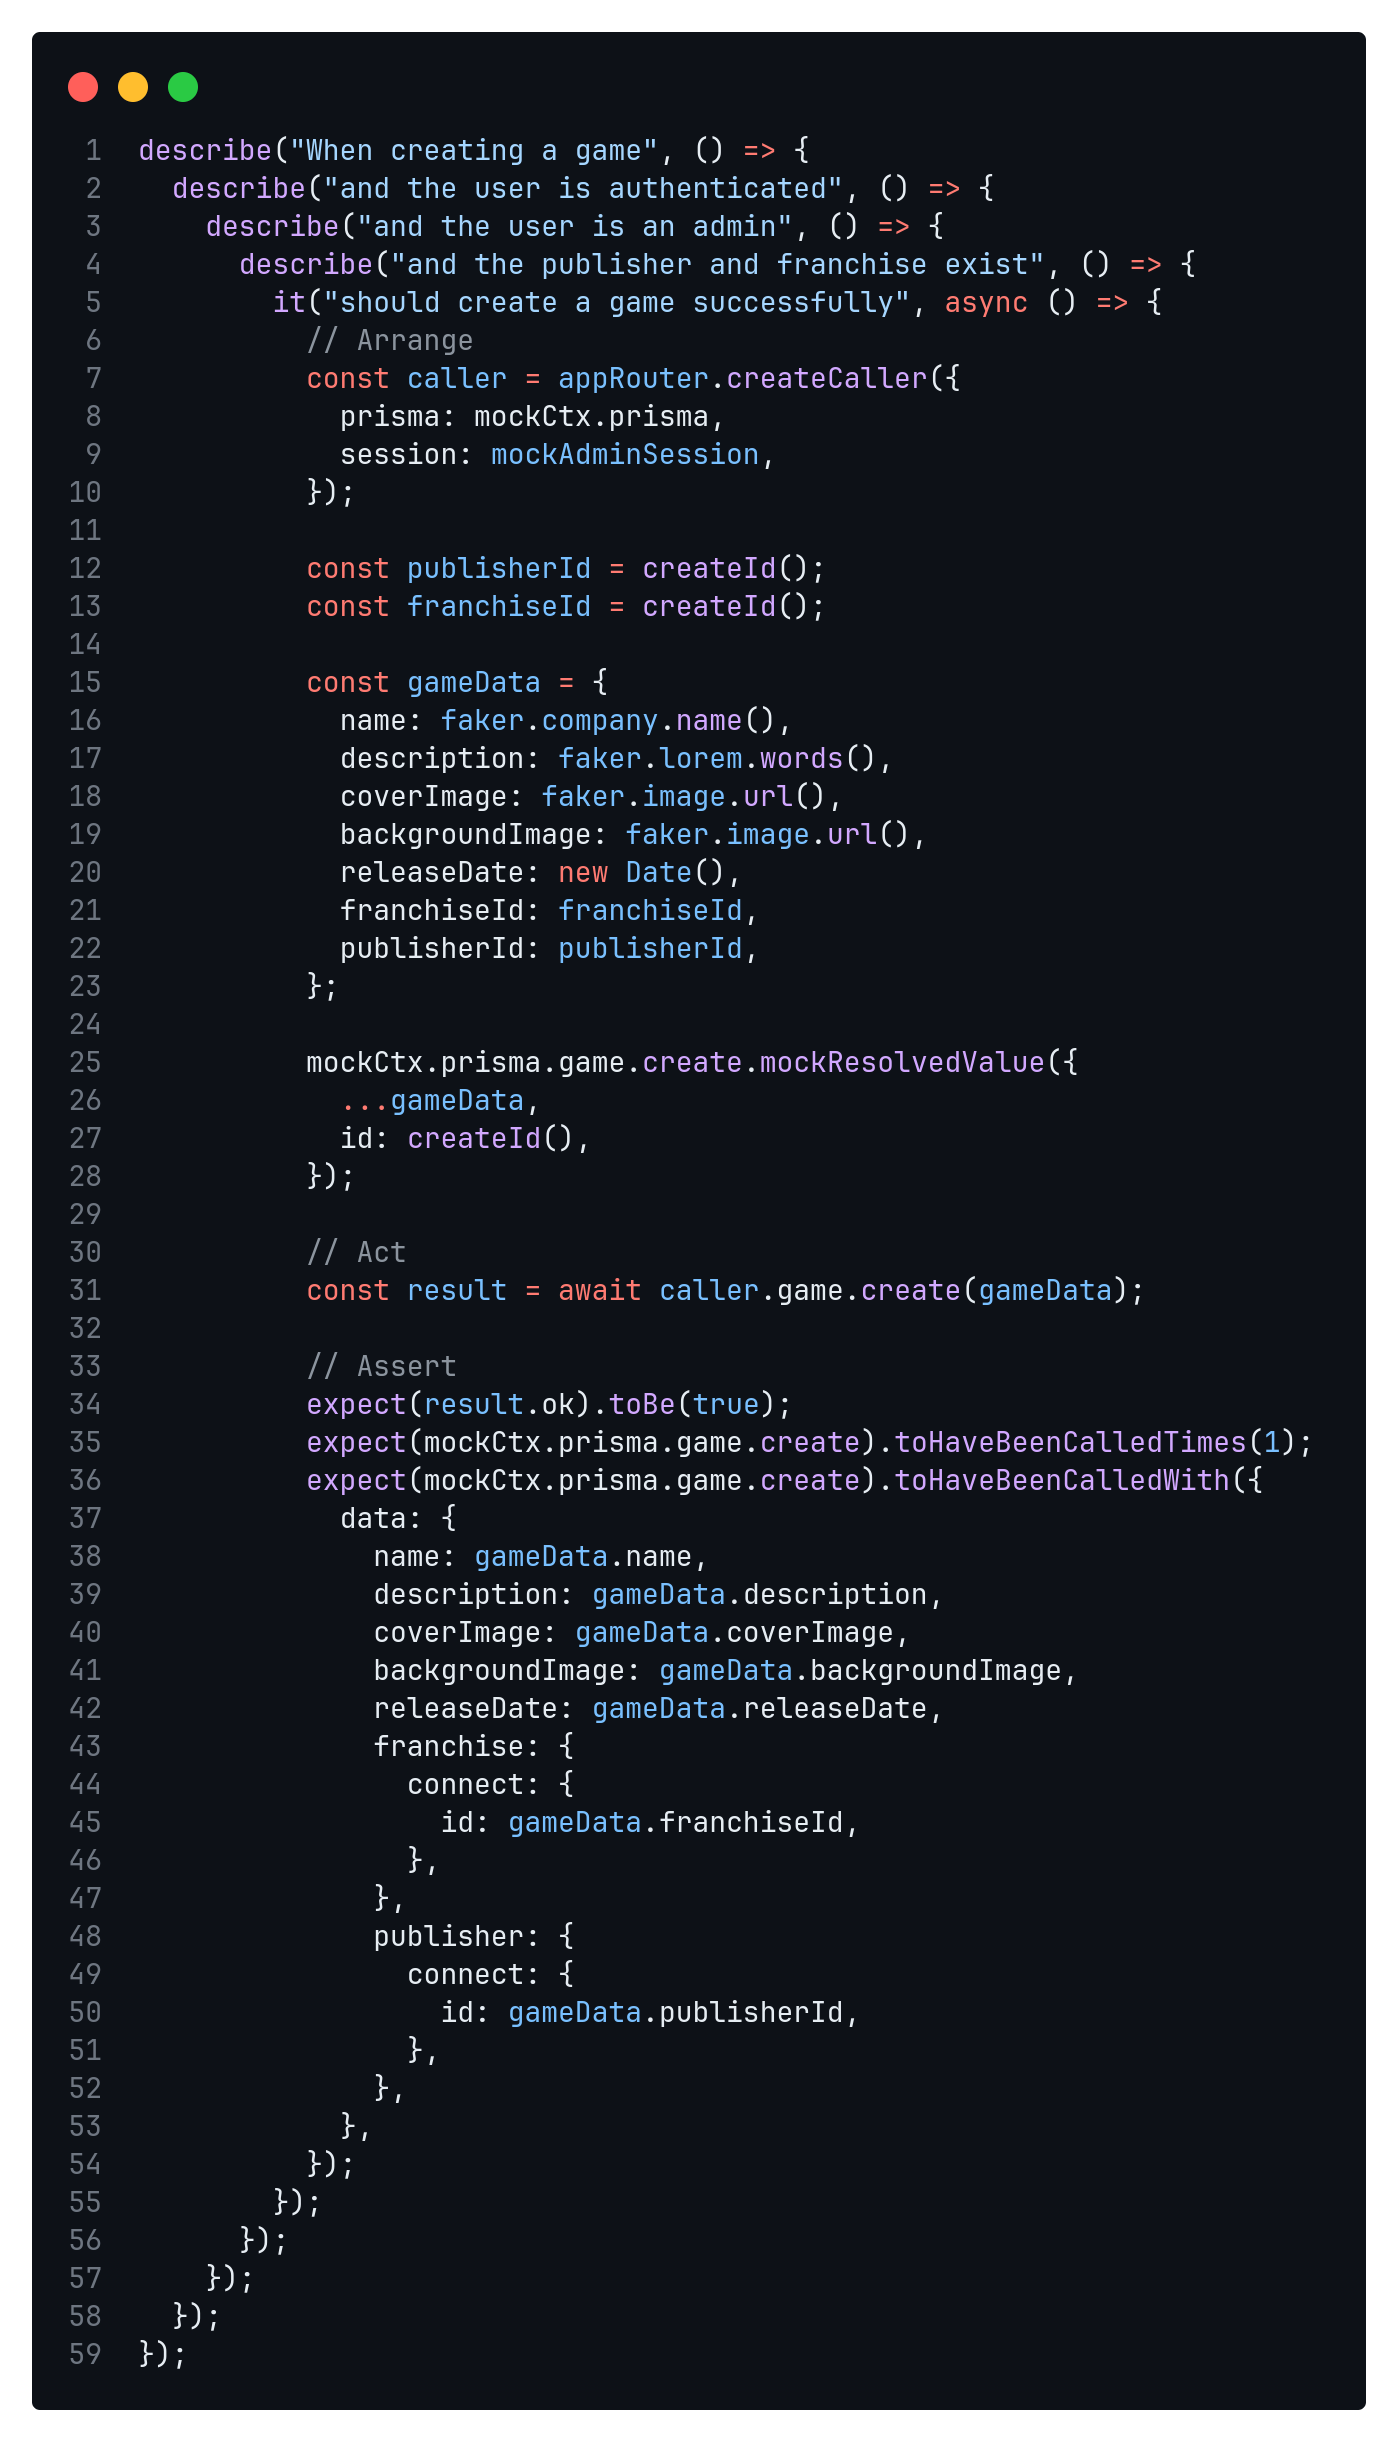
\includegraphics[height=\dimexpr
        \textheight-3\baselineskip-\parskip-.2em-
      \abovecaptionskip-\belowcaptionskip\relax]{test_unit.png}
      \caption{Παράδειγμα ελέγχου μονάδας για την επιτυχημένη δημιουργία
      παιχνιδιού}
    \end{center}
    \label{fig:TestUnit}
  \end{figure}

  \begin{figure}[H]
    \begin{center}
      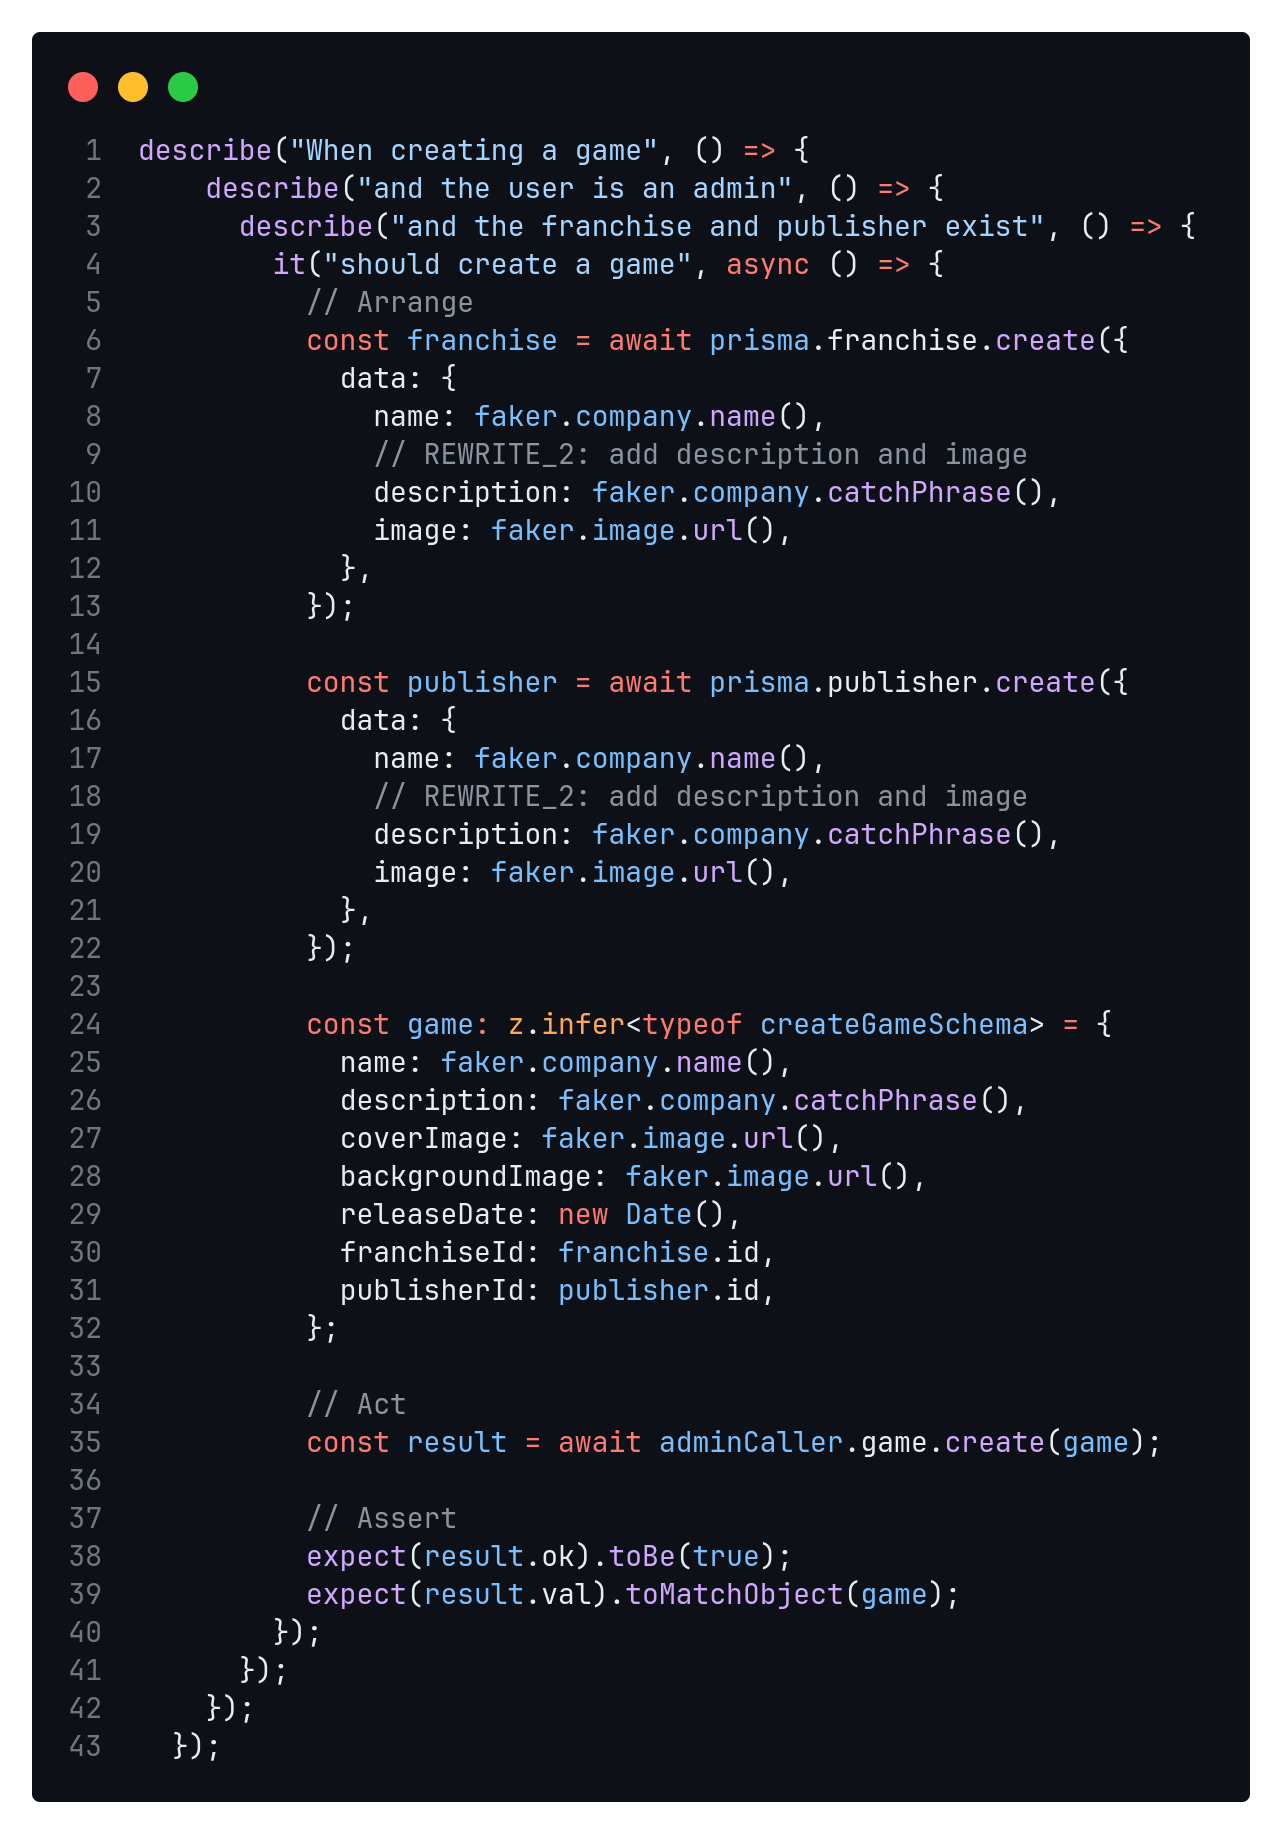
\includegraphics[height=\dimexpr
        \textheight-3\baselineskip-\parskip-.2em-
      \abovecaptionskip-\belowcaptionskip\relax]{test_integration.png}
      \caption{Παράδειγμα ελέγχου συμαβότητας για την επιτυχημένη
      δημιουργία παιχνιδιού}
    \end{center}
    \label{fig:TestIntegration}
  \end{figure}

  Εκ πρώτης όψεως, ο κώδικας στο Σχήμα \ref{fig:TestUnit} φαίνεται να
  είναι πιο περίπλοκος αυτού στο Σχήμα \ref{fig:TestIntegration}, ωστόσο,
  στην περίπτωση του ελέγχου μονάδας, οι εξαρτήσεις είναι προσομοιωμένες.
  Δεν υπάρχει κάποιος πραγματικός χρήστης, ή κάποια πραγματική βάση
  δεδομένων. Αντίθετα, στην περίπτωση του ελέγχου συμβατότητας, οι
  εξαρτήσεις είναι πραγματικές, και ο έλεγχος πρέπει να ελέγξει την
  συμβατότητα του συστήματος με μια πραγματική βάση δεδομένων, ένα
  πραγματικό χρήστη και μετά από τον κάθε έλεγχο, πρέπει να είναι σίγουρο
  ότι εσωτερική κατάσταση του προγράμματος και της βάσης είναι κοινή για
  όλες τις περιπτώσεις, αποφεύγοντας περιπτώσεις ασταθών δοκιμών
  (\textlatin{flaky tests}), όπου το αποτέλεσμα της δοκιμής δεν είναι
  πάντοτε αμετάβλητο. \cite{Parry2022}

  \section{Αξιολόγηση Απαντήσεων}

  Κατά την αλληλεπίδραση με το μοντέλο, για κάθε απάντηση που δόθηκε
  έπειτα προτροπής, πραγματοποιήθηκε μια αξιολόγηση σε μια κλίμακα μεταξύ
  μείον δύο (-2) και δύο (2), με το μείον δύο να αντιστοιχεί σε μια
  απάντηση η οποία κρίθηκε ως εντελώς λάθος, το μείον ένα (-1) σε μια
  απάντηση η οποία κρίθηκε ως μερικώς λάθος, το μηδέν (0) σε μια απάντηση
  η οποία κρίθηκε ως αδιάφορη προς την ορθότητά της, το ένα (1) σε μια
  απάντηση η οποία κρίθηκε ως σωστή και το δύο (2) σε μια απάντηση η οποία
  κρίθηκε ως εντελώς σωστή.

  Η επιλογή μιας κλίμακας η οποία εκτείνεται από \say{πολύ κακό} έως
  \say{πολύ καλό}, αποσκοπεί στην καλύτερη αναπαράσταση της ποικιλίας και
  της πολυπλοκότητας της αξιολόγησης μιας απάντησης και στην δημιουργία
  ενός συνόλου ασαφούς λογικής (\textlatin{fuzzy logic}) για την
  αξιολόγηση των απαντήσεων
  \cite{ZADEH1965338,klir1995fuzzy,ross2010fuzzy}.

  Η αξιολόγηση των απαντήσεων αποσκοπεί στην εξάσκηση ενός μοντέλου
  μηχανικής μάθησης, προκειμένου να βελτιωθεί η απόδοσή του στην παραγωγή
  απαντήσεων, με βάση την ορθότερη προτροπή, του οποίου η ανάλυση γίνεται
  στο επόμενο κεφάλαιο.

  \begin{figure}[H]
    \begin{center}
      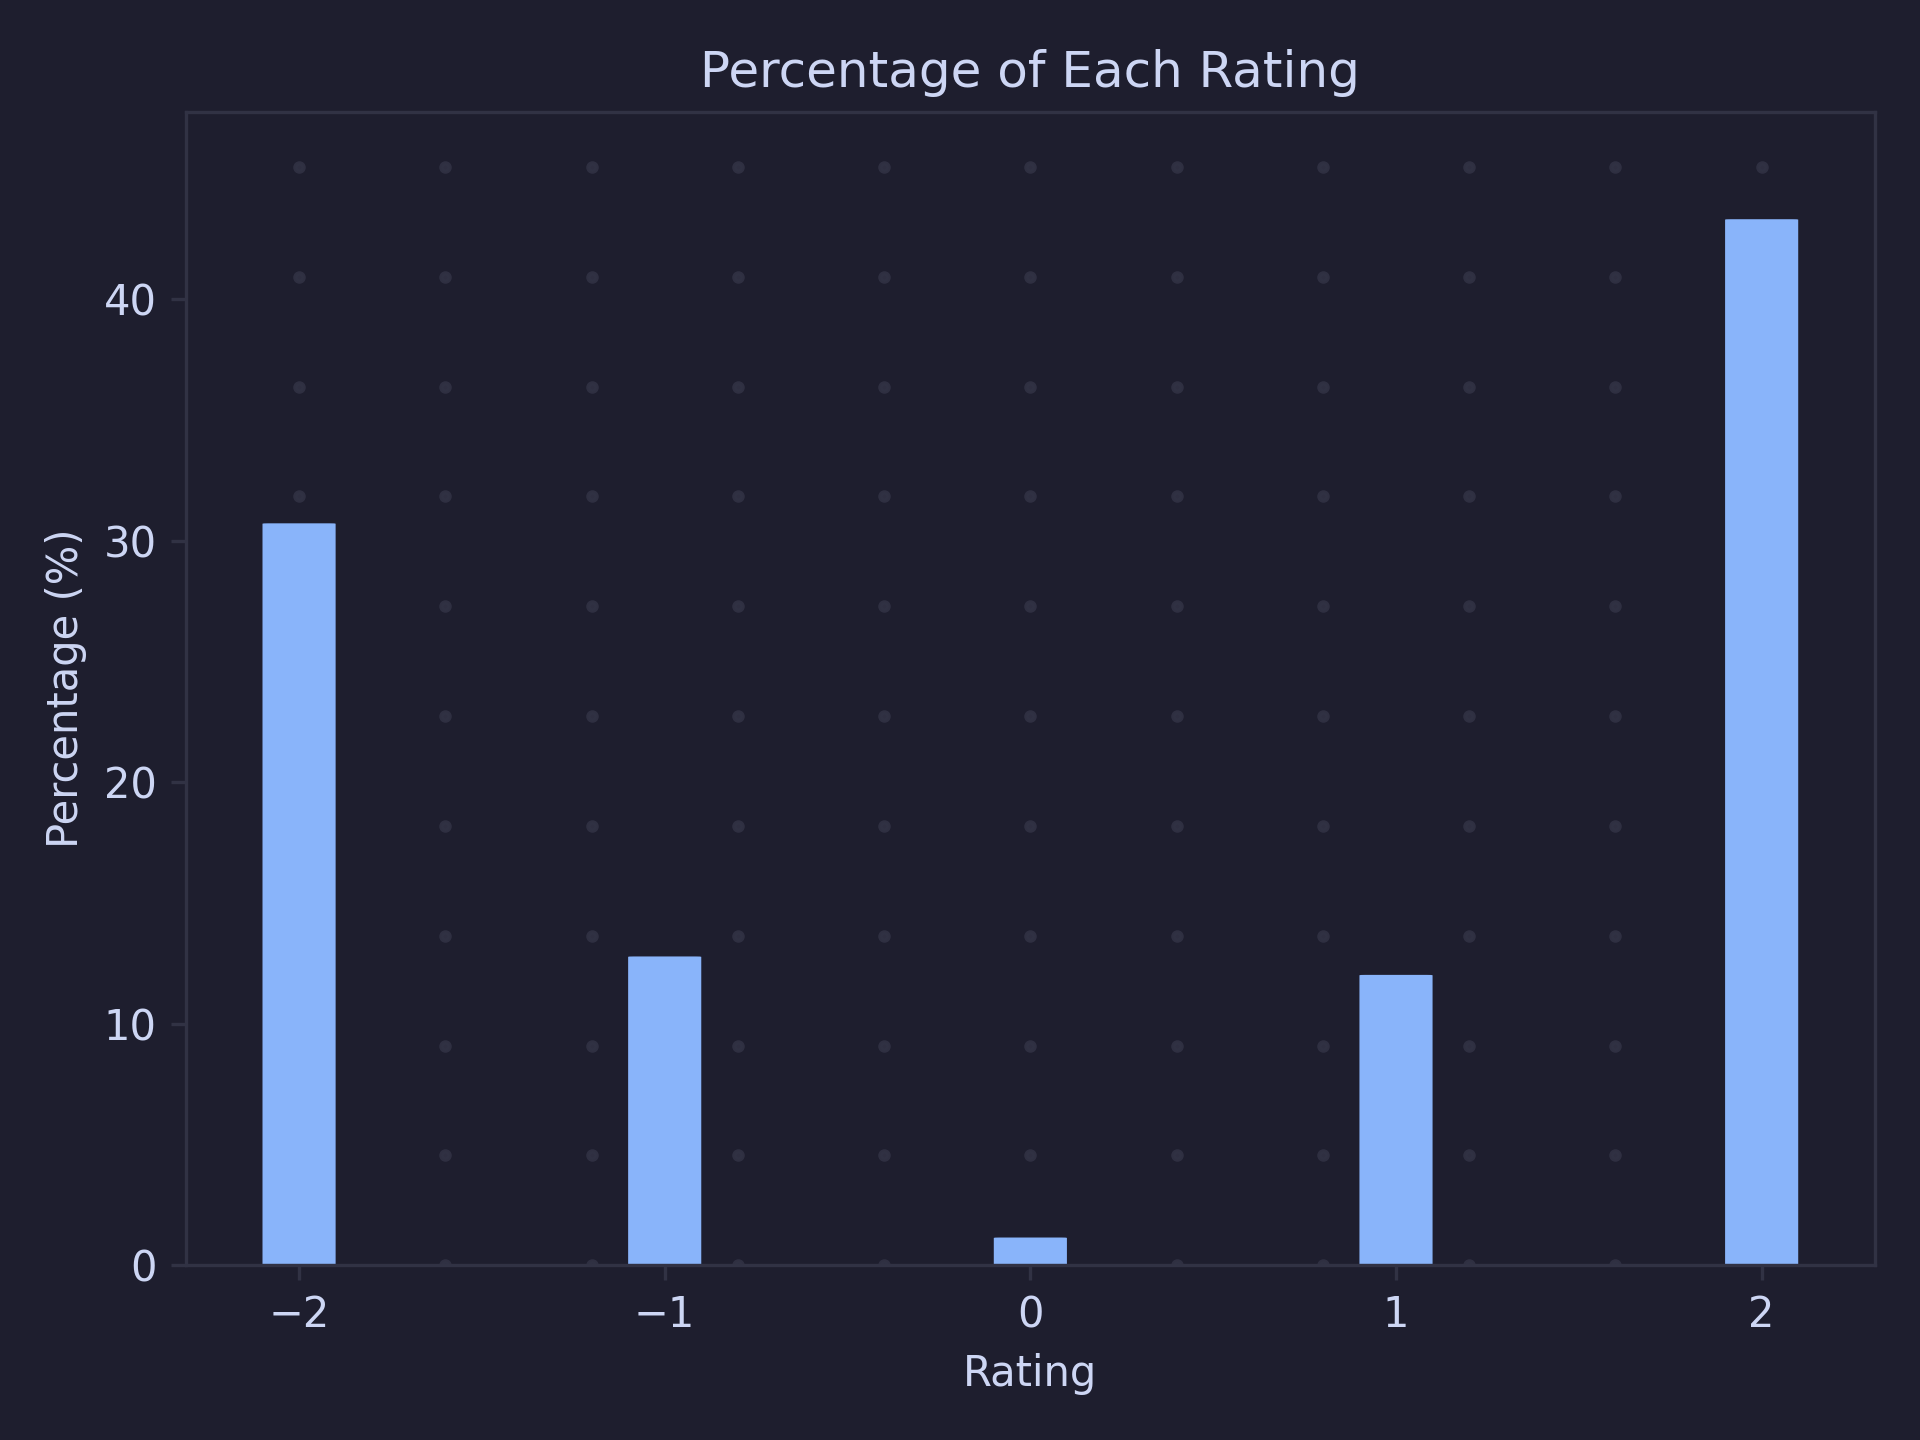
\includegraphics[width=0.85\textwidth]{rating_perc.png}
      \caption{Ποσοστό αξιολόγησης απαντήσεων}
    \end{center}
    \label{fig:RatingPerc}
  \end{figure}

  \begin{figure}[H]
    \begin{center}
      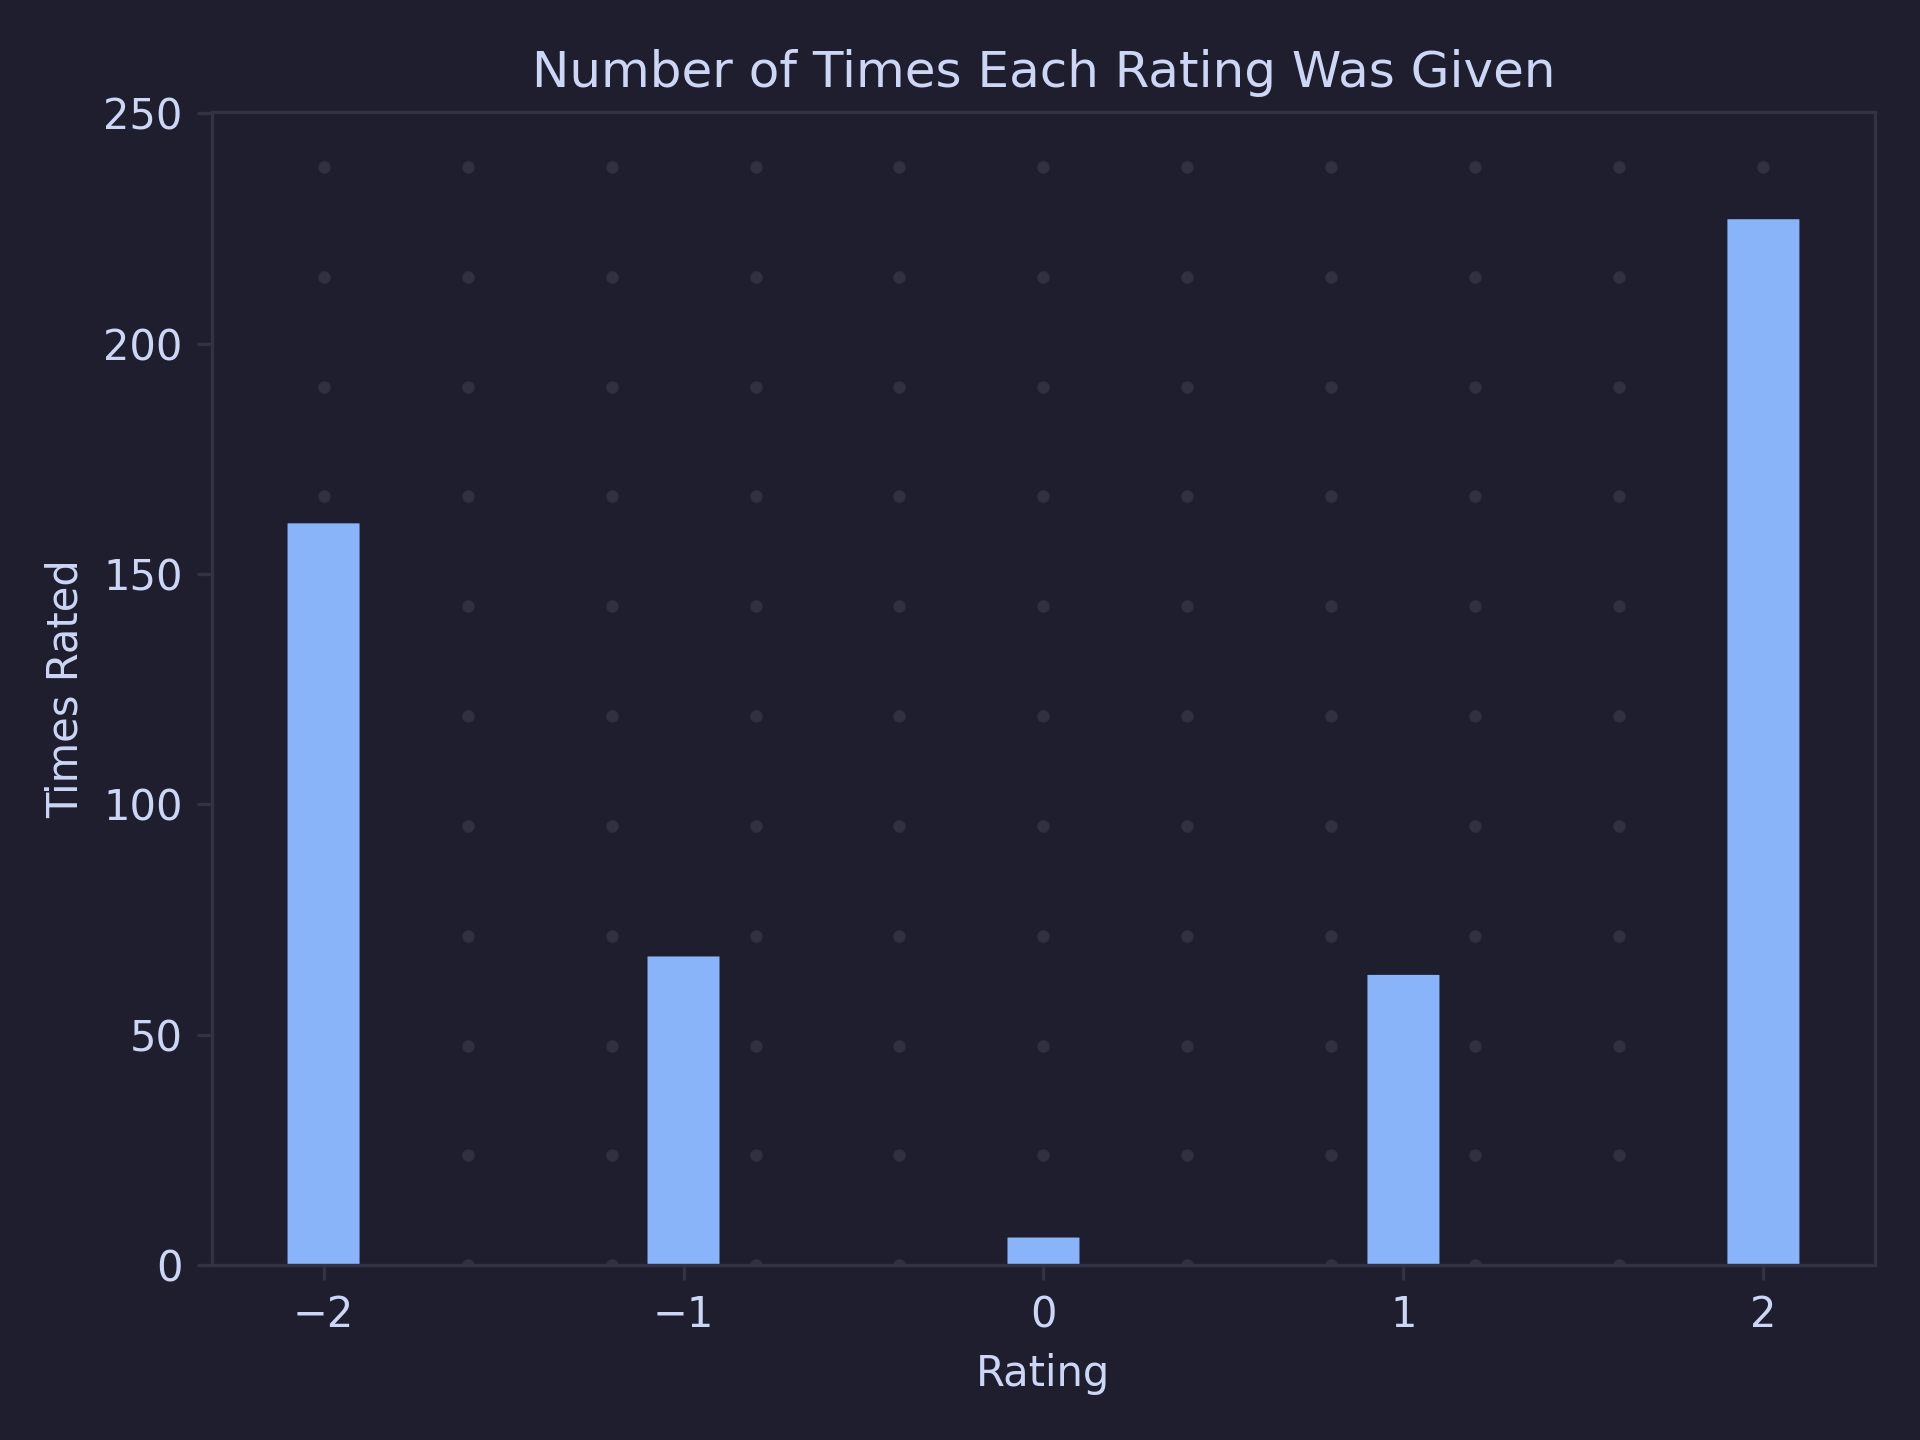
\includegraphics[width=0.85\textwidth]{rating_times.png}
      \caption{Αριθμός αξιολόγησης απαντήσεων}
    \end{center}
    \label{fig:RatingTimes}
  \end{figure}

  Από τα σχήματα \ref{fig:RatingPerc} και \ref{fig:RatingTimes},
  παρατηρείται ότι η πλειοψηφία των απαντήσεων αξιολογήθηκαν θετικά, με το
  το πενήντα πέντε τοις εκατό (55.3435\%), με σύνολο 290 θετικών
  αξιολογήσεων, έναντι του σαράντα τρία τοις εκατό (43.5115\%), με με
  σύνολο 228 αρνητικών αξιολογήσεων. Ο συνηθέστερος βαθμός αξιολόγησης
  ήταν το δύο (2), με σύνολο διακοσίων εικοσιεπτά (227) αξιολογήσεων, ενώ
  ο σπανιότερος βαθμός αξιολόγησης ήταν το μηδέν (0), με σύνολο έξι (6)
  αξιολογήσεων.

  \begin{figure}[H]
    \begin{center}
      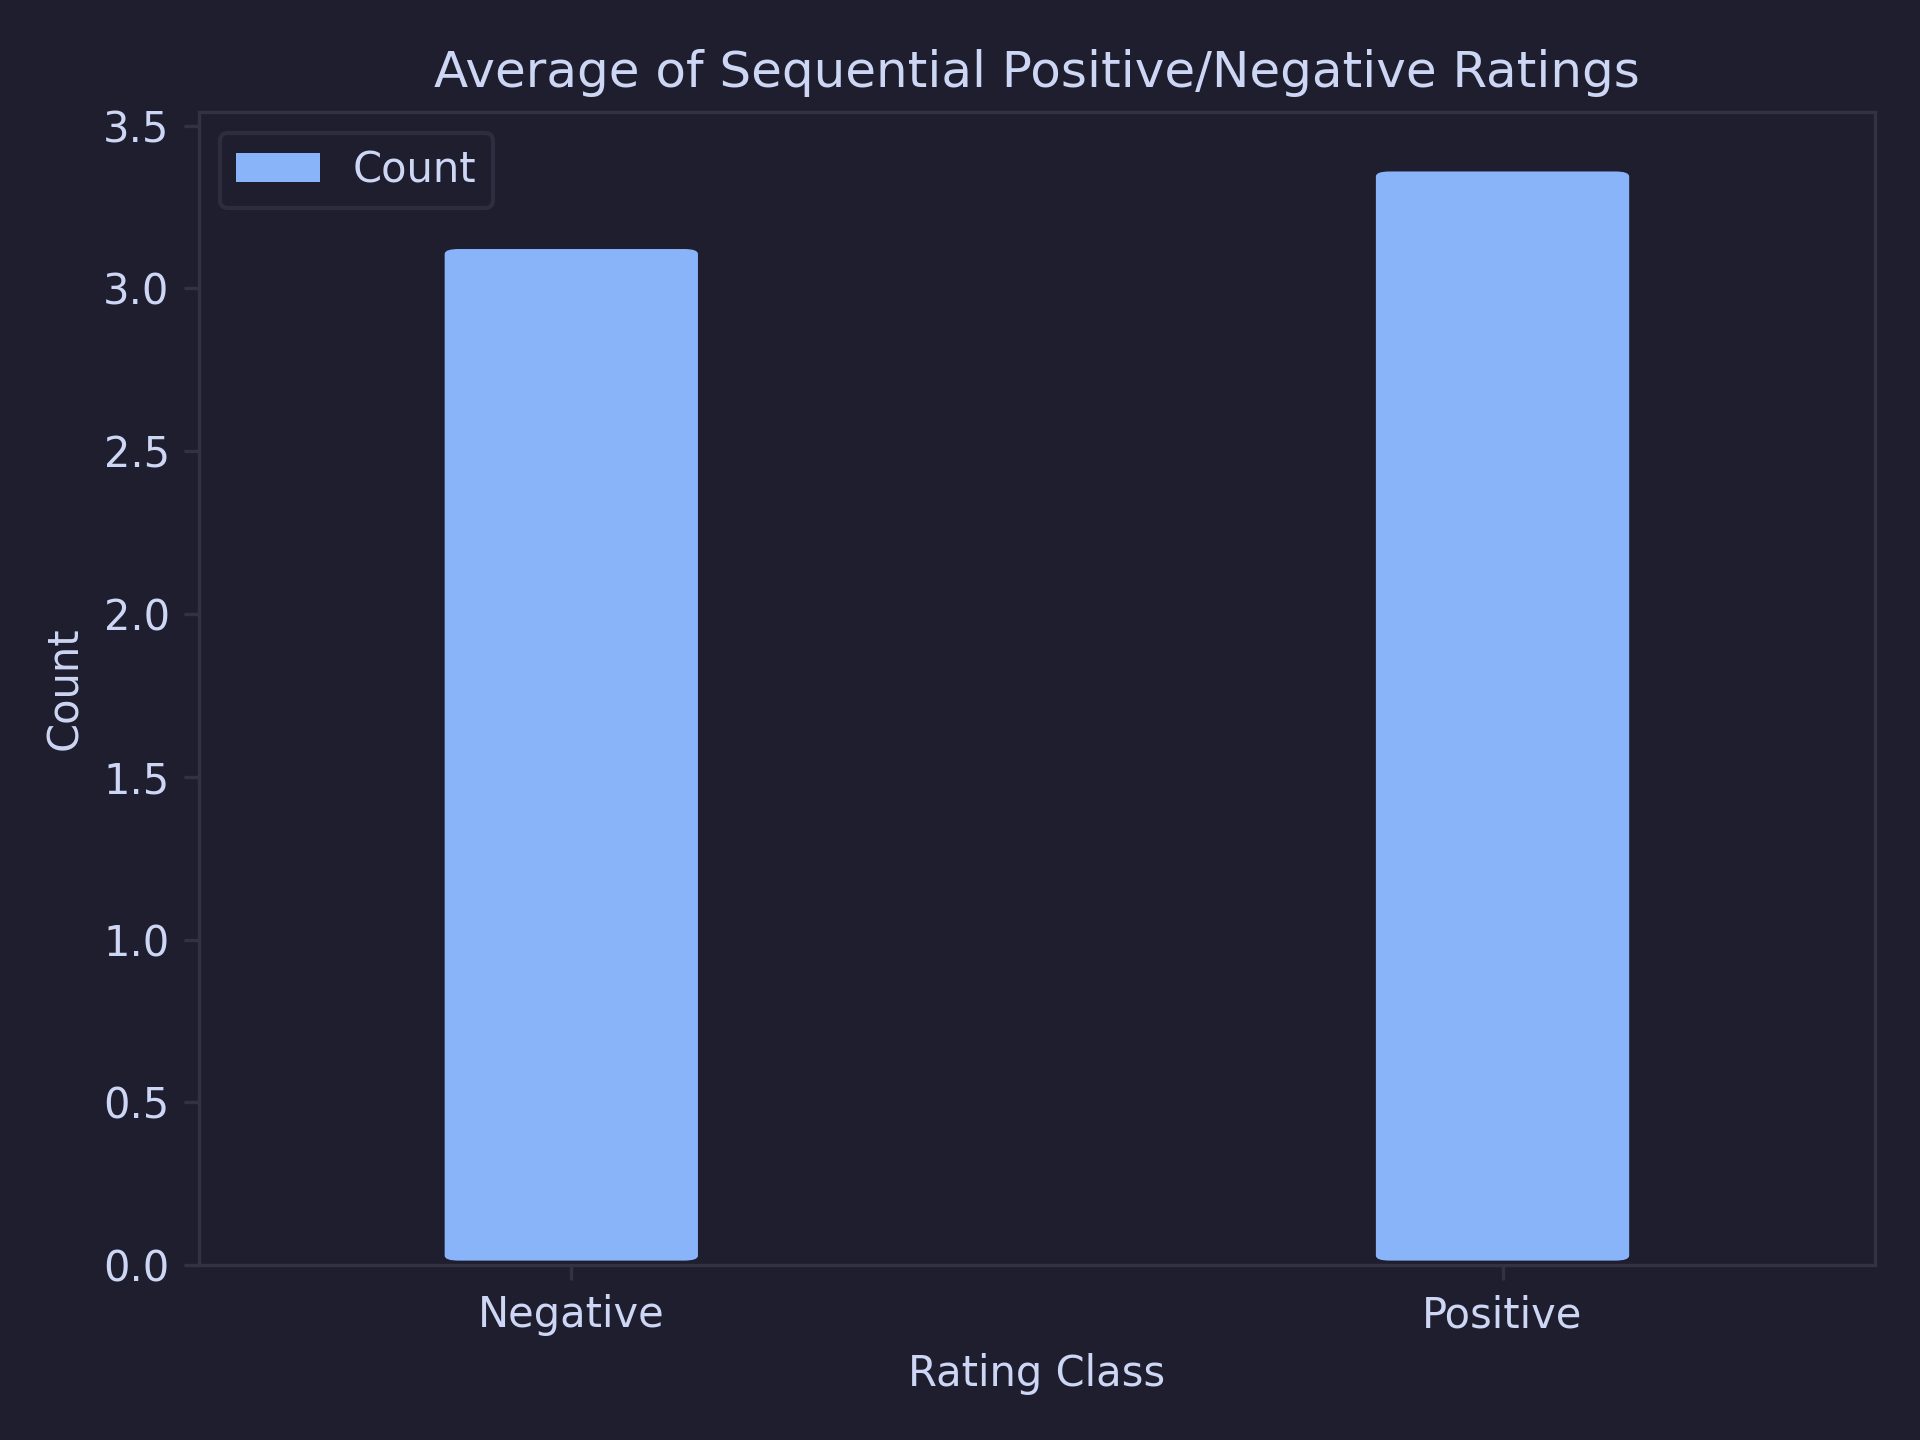
\includegraphics[width=0.7\textwidth]{avg_sequential.png}
      \caption{Μέσος όρος συνεχόμενης αξιολόγησης απαντήσεων}
    \end{center}
    \label{fig:AverageSequential}
  \end{figure}

  \begin{figure}[H]
    \begin{center}
      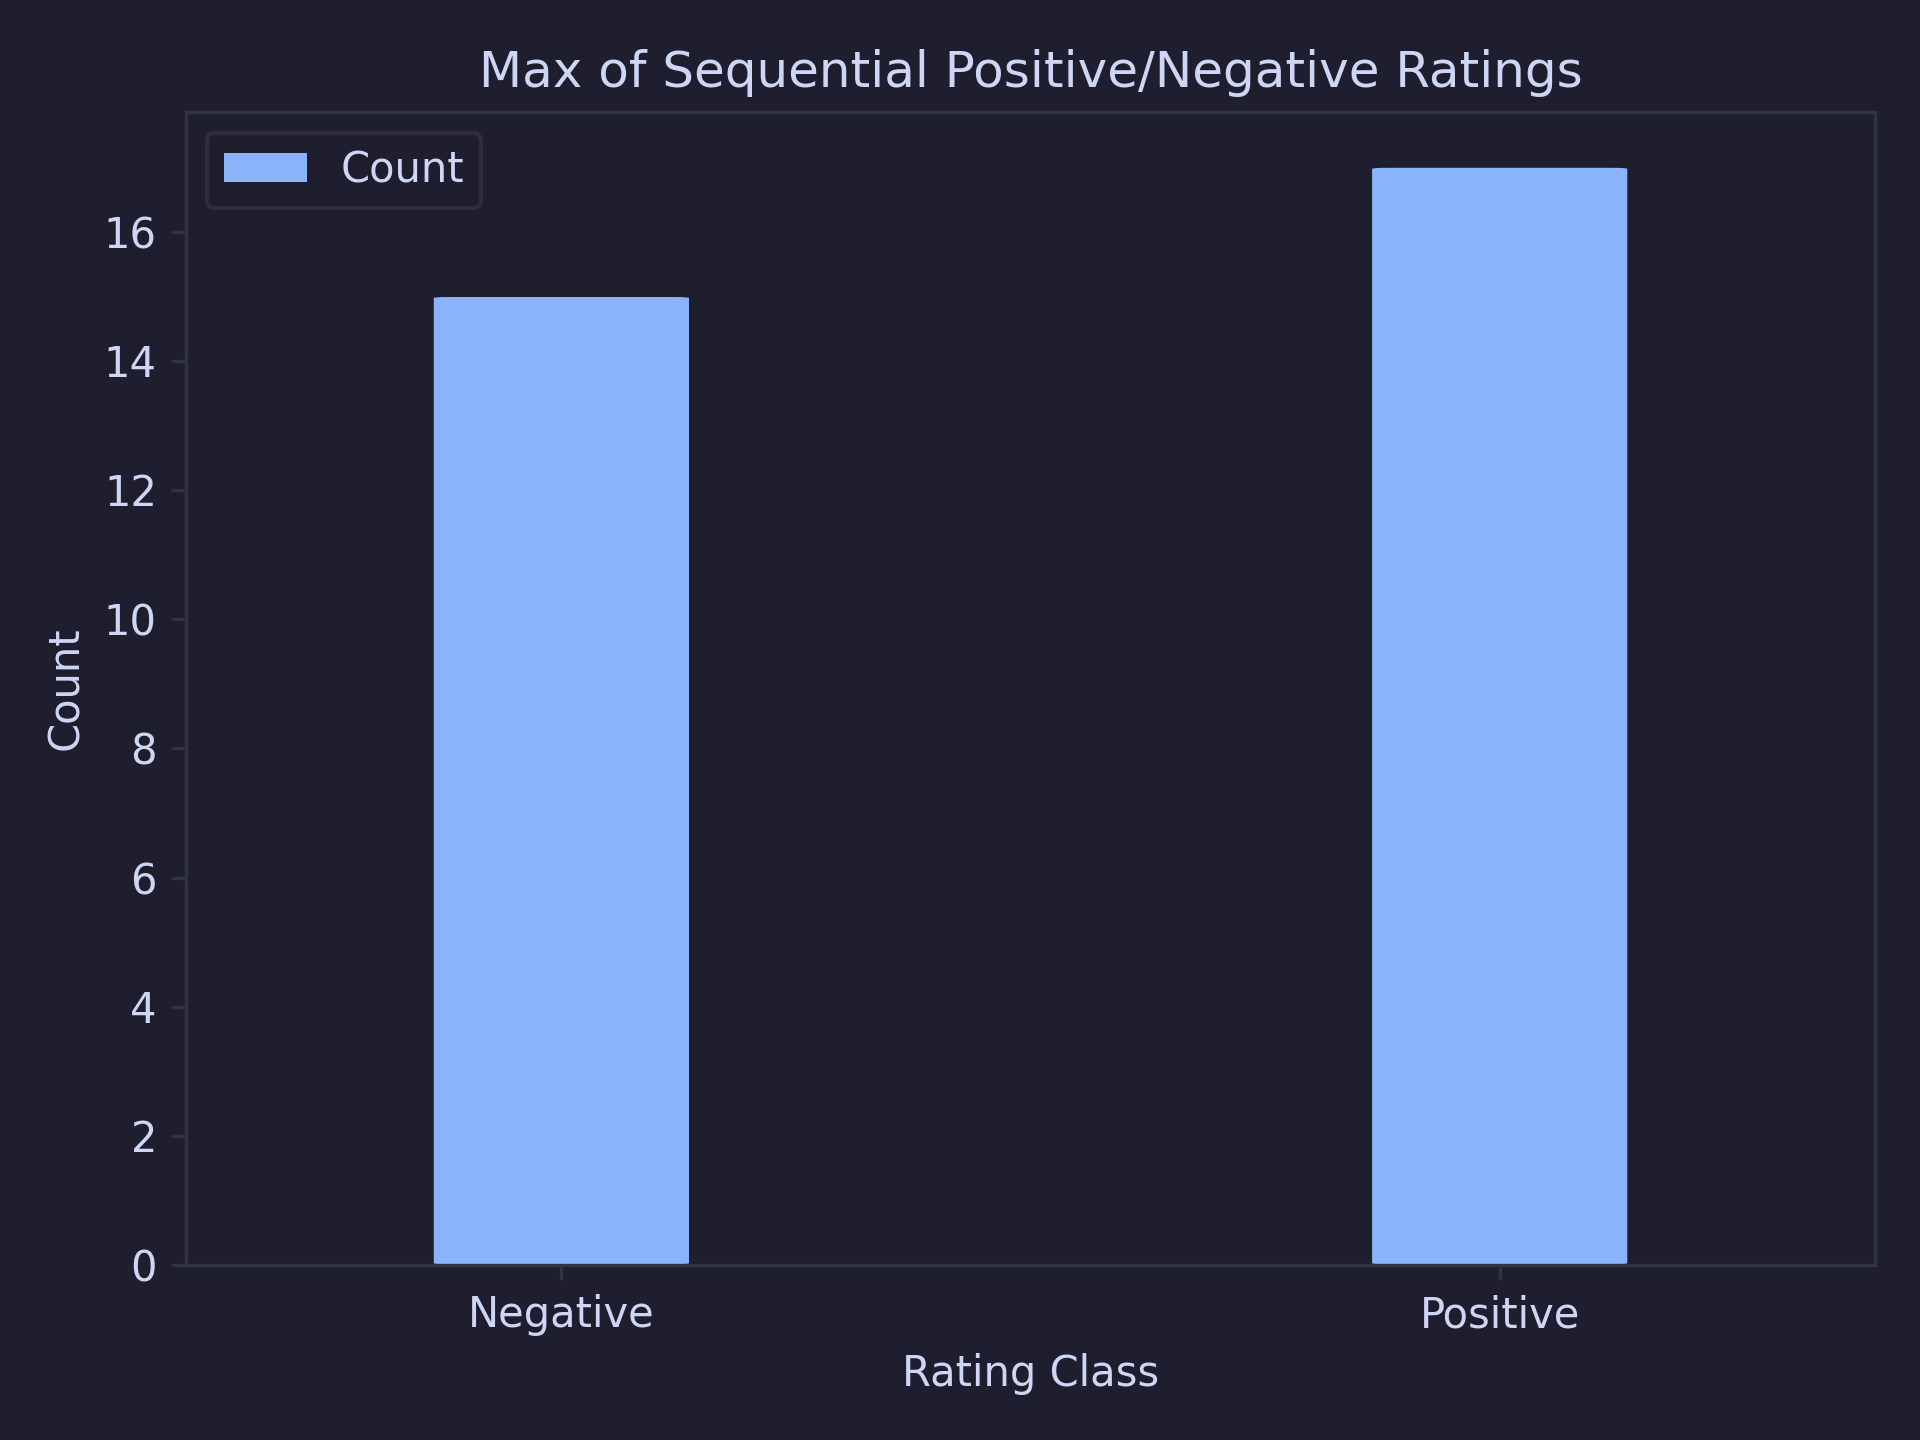
\includegraphics[width=0.7\textwidth]{max_sequential.png}
      \caption{Μέγιστη συνεχόμενη αξιολόγηση απαντήσεων}
    \end{center}
    \label{fig:MaxSequential}
  \end{figure}

  Το μοντέλο φαίνεται να έχει την τάση να παράγει απαντήσεις οι οποίες
  βασίζονται πολύ στην αρχική παρότρυνση από την προτροπή του
  προγραμματιστή. Αυτό αποδεικνύεται και από το σχήμα
  \ref{fig:MaxSequential}, όπου παρατηρείται ότι ο μέγιστος αριθμός
  συνεχόμενων αρνητικών αξιολογήσεων είναι δεκατέσσερεις (14), ενώ ο
  μέγιστος αριθμός συνεχόμενων θετικών αξιολογήσεων είναι δεκατρείς (16).
  Στην περίπτωση των συνεχόμενων θετικών αξιολογήσεων, οι προτροπές
  αφορούσαν 3 διαφορετικά θέματα, τους ελέγχους της λειτουργίας των
  κριτικών, την ανάπτυξη της λειτουργίας των λιστών, καθώς και τους
  ελέγχους της. Στην περίπτωση των συνεχόμενων αρνητικών αξιολογήσεων, οι
  προτροπές αφορούσαν μόνο τους ελέγχους μιας λειτουργίας.

  \begin{figure}[H]
    \begin{center}
      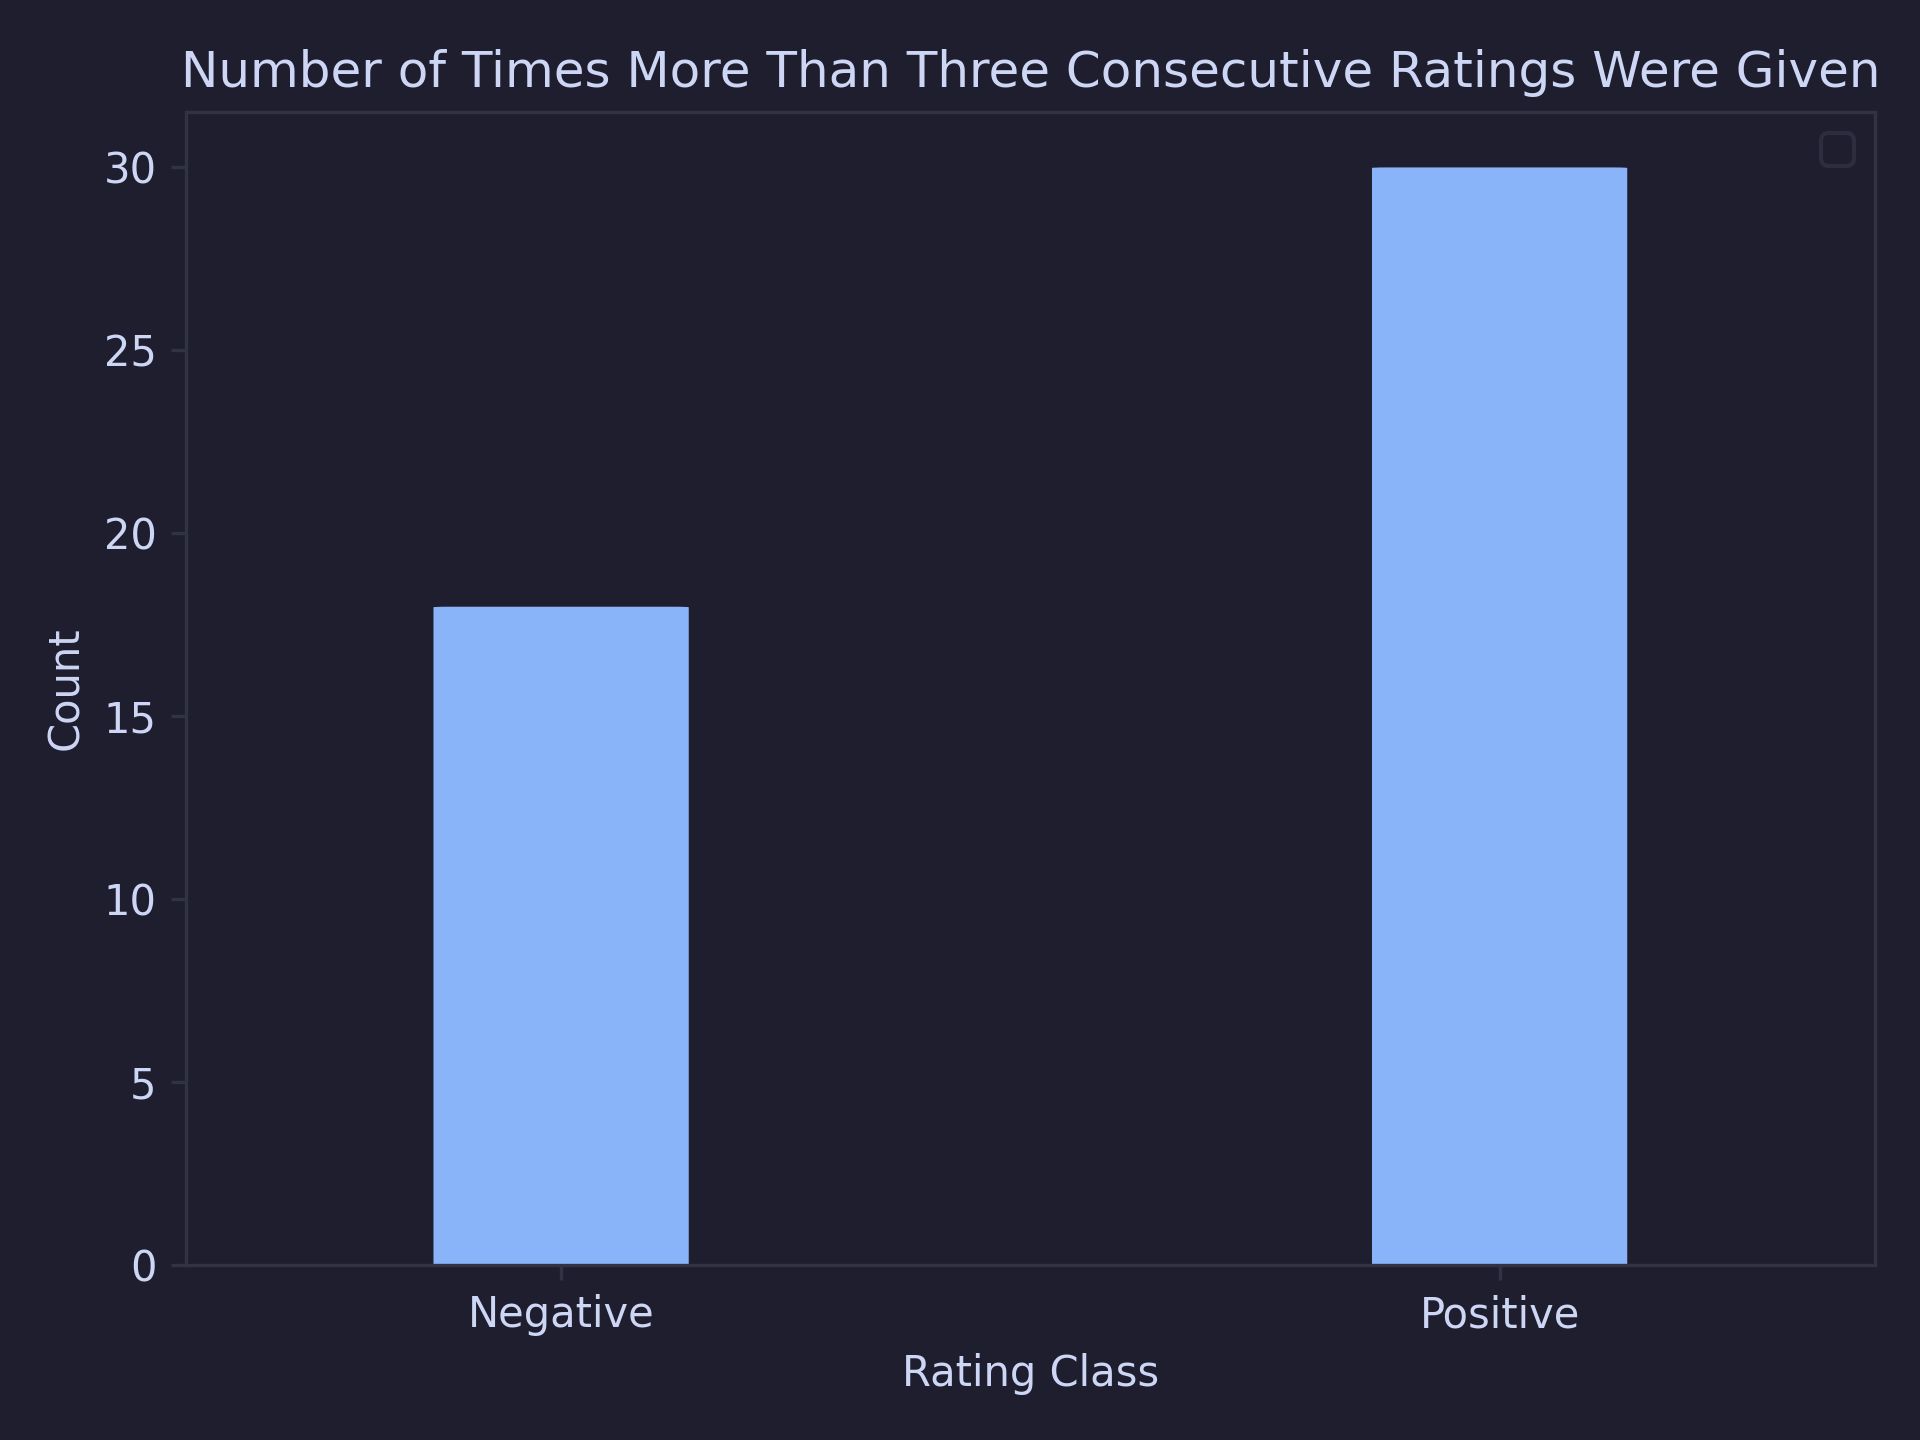
\includegraphics[width=0.7\textwidth]{consecutive_streaks.png}
      \caption{Αριθμός εμφανίσεων συνεχόμενων αξιολογήσεων άνω των τριών
      (3)}
    \end{center}
    \label{fig:ConsecutiveStreaks}
  \end{figure}

  \begin{figure}[H]
    \begin{center}
      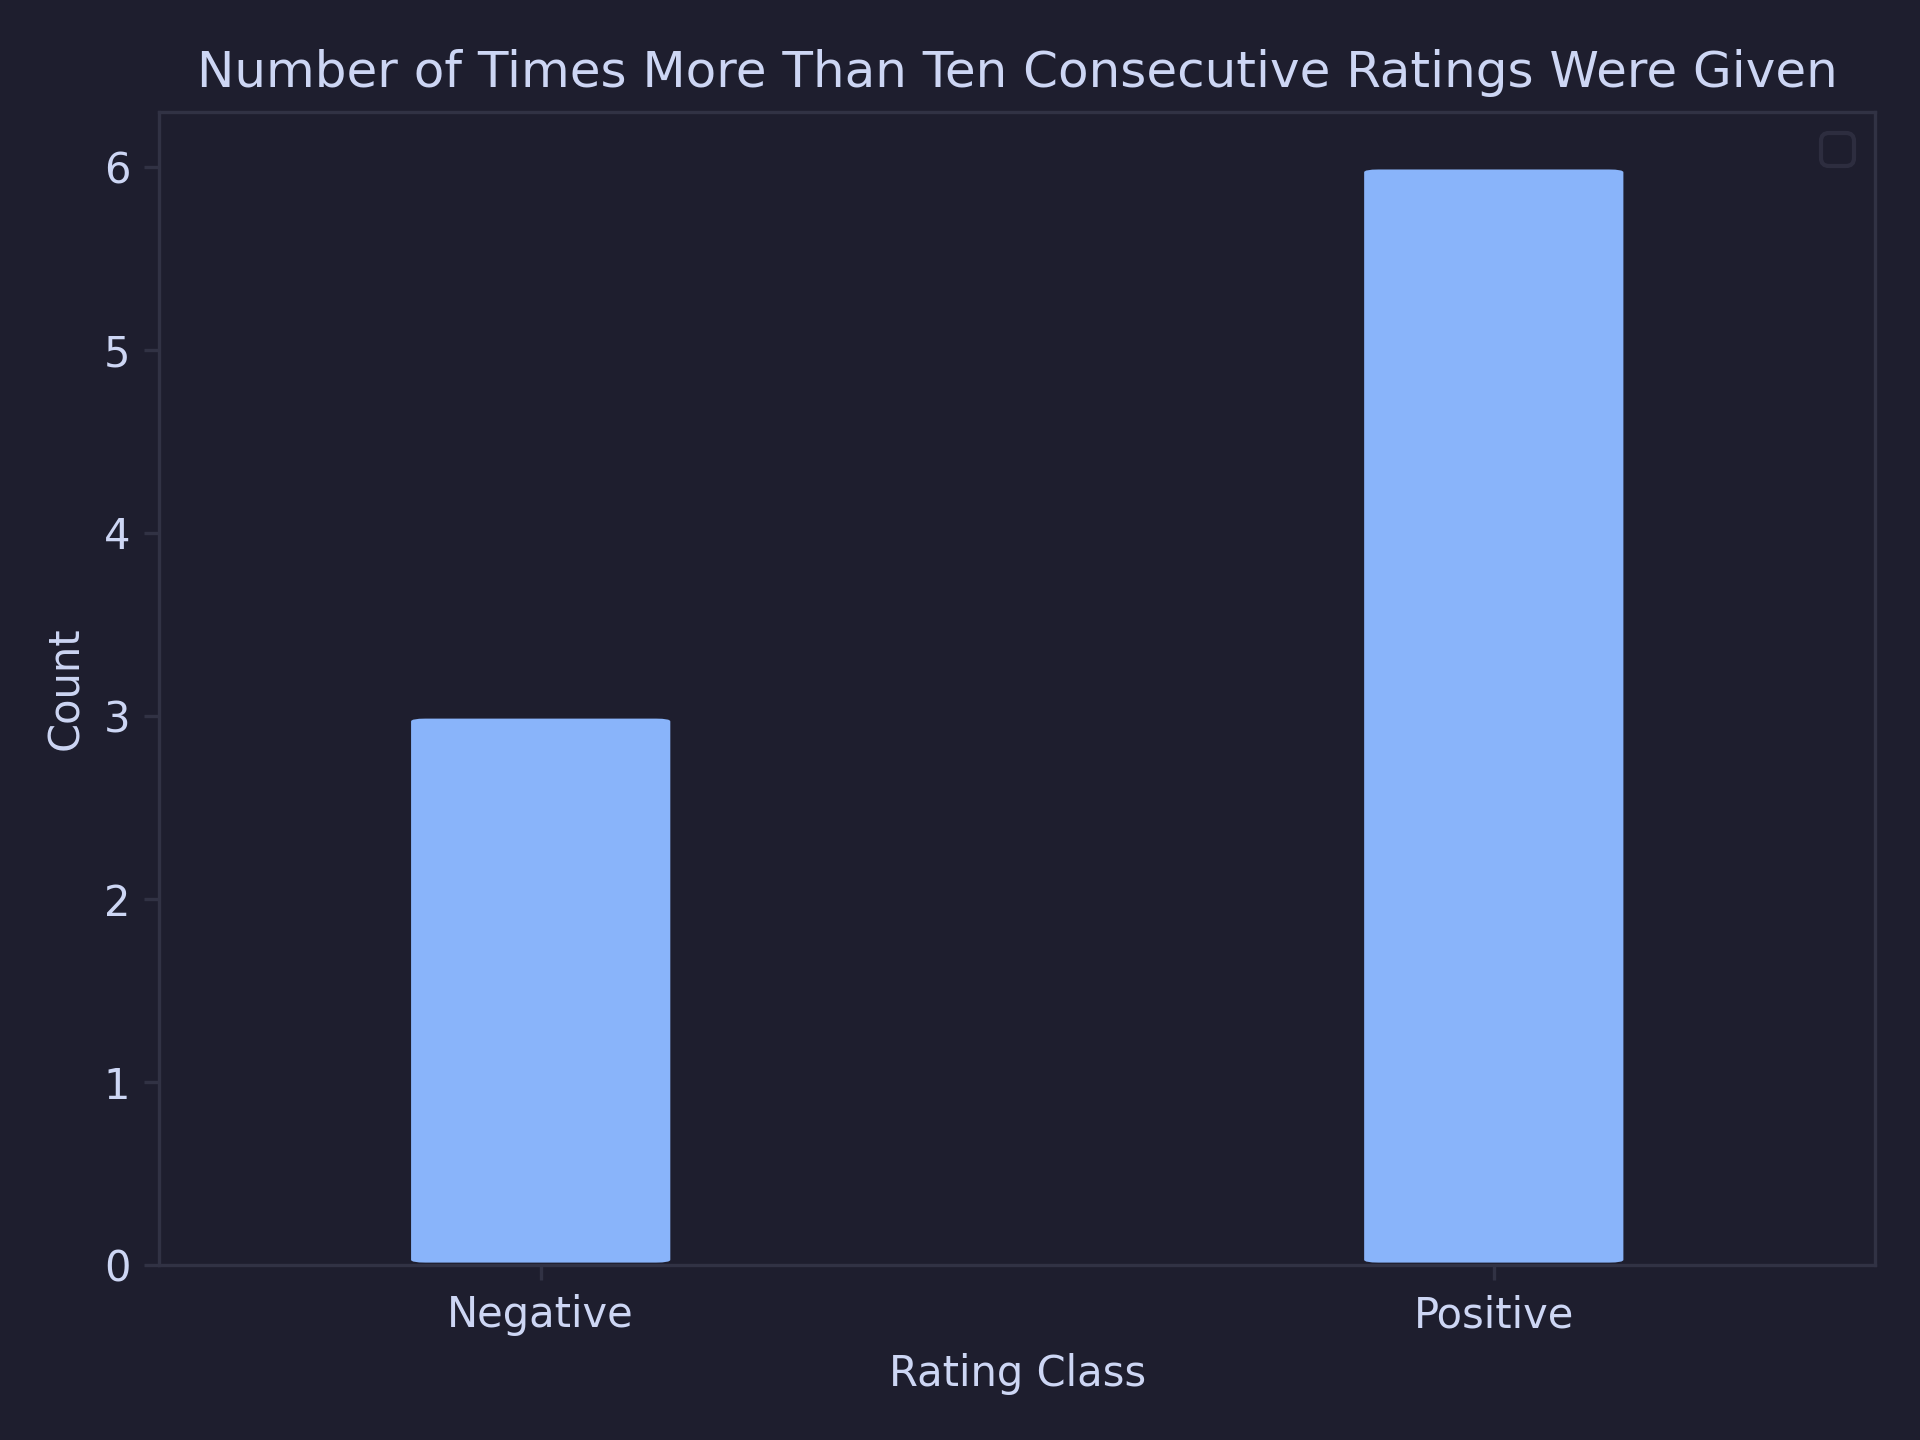
\includegraphics[width=0.7\textwidth]{consecutive_streaks_more_than_10.png}
      \caption{Αριθμός εμφανίσεων συνεχόμενων αξιολογήσεων άνω των δέκα
      (10)}
    \end{center}
    \label{fig:ConsecutiveStreaks10}
  \end{figure}

  Για την περίπτωση των άνω των δέκα (10) συνεχόμενων θετικών
  αξιολογήσεων, κατά μέσο όρο, αφορούσαν δύο (2) διαφορετικά θέματα, ενώ
  ήταν διπλάσιες οι περιπτώσεις εμφάνισης των συνεχόμενων θετικών έναντι
  των αρνητικών αξιολογήσεων (\ref{fig:ConsecutiveStreaks10}), που
  αφορούσαν ένα θέμα. Φαίνεται πως αν η πρώτη προτροπή από τον
  προγραμματιστή δεν οδηγήσει ορθά το μοντέλο, τότε δύσκολα βρίσκει τη
  λύση με τις επόμενες προτροπές, καθώς διατηρείται η αρχική κατεύθυνση
  που έλαβε.

  \begin{figure}[H]
    \begin{center}
      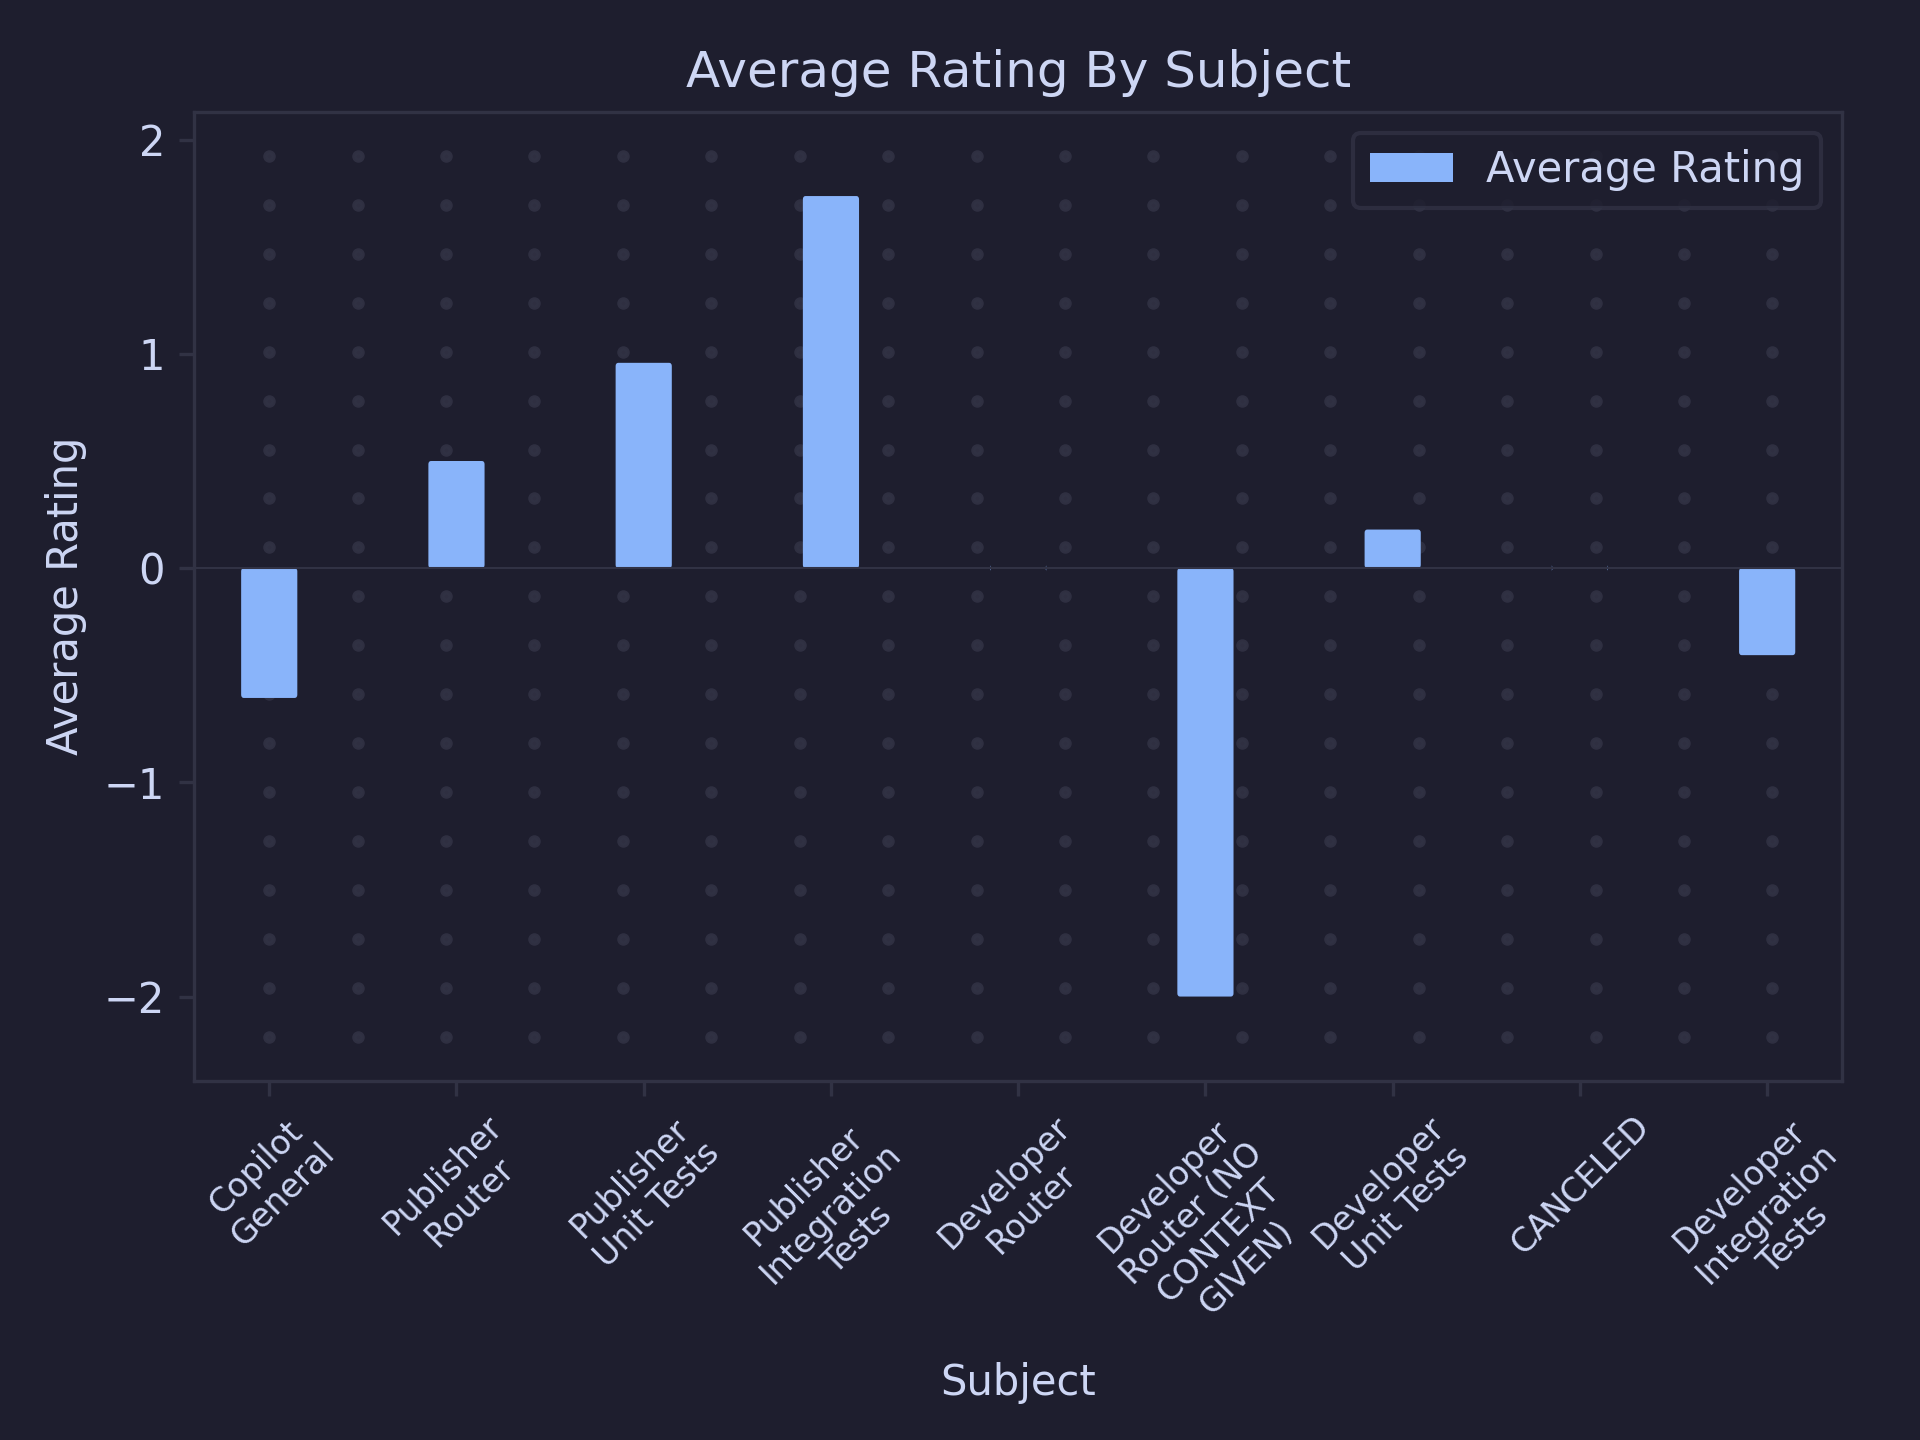
\includegraphics[width=0.85\textwidth]{subject_query_1.png}
      \caption{Μέσος όρος αξιολόγησης απαντήσεων για θέματα, \textit{μέρος
      1}}
    \end{center}
    \label{fig:SubjectQuery1}
  \end{figure}

  \begin{figure}[H]
    \begin{center}
      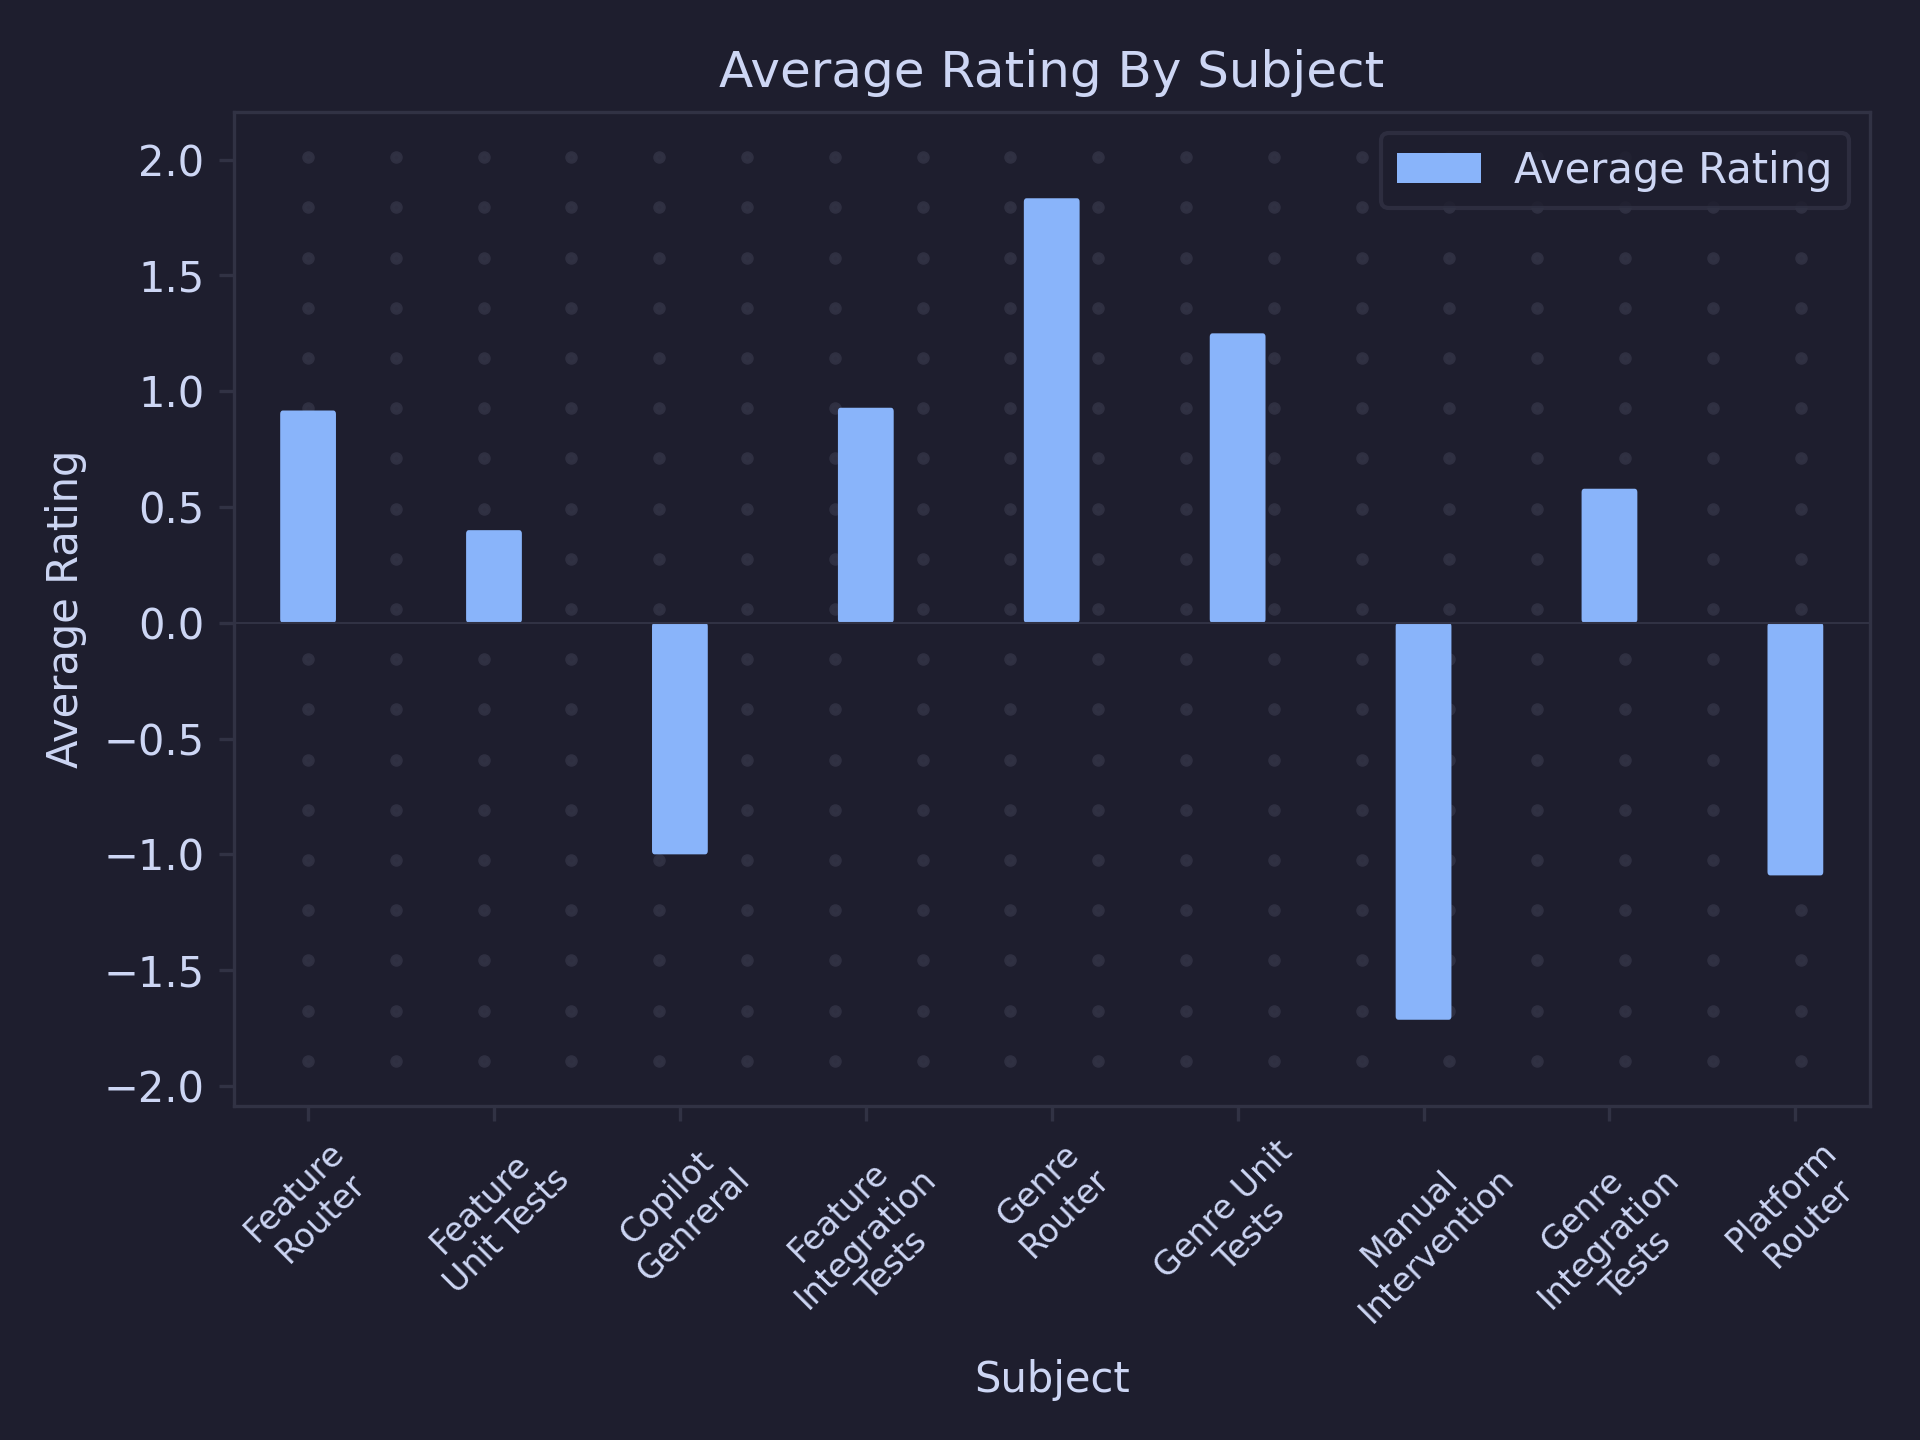
\includegraphics[width=0.85\textwidth]{subject_query_2.png}
      \caption{Μέσος όρος αξιολόγησης απαντήσεων για θέματα, \textit{μέρος
      2}}
    \end{center}
    \label{fig:SubjectQuery2}
  \end{figure}

  \begin{figure}[H]
    \begin{center}
      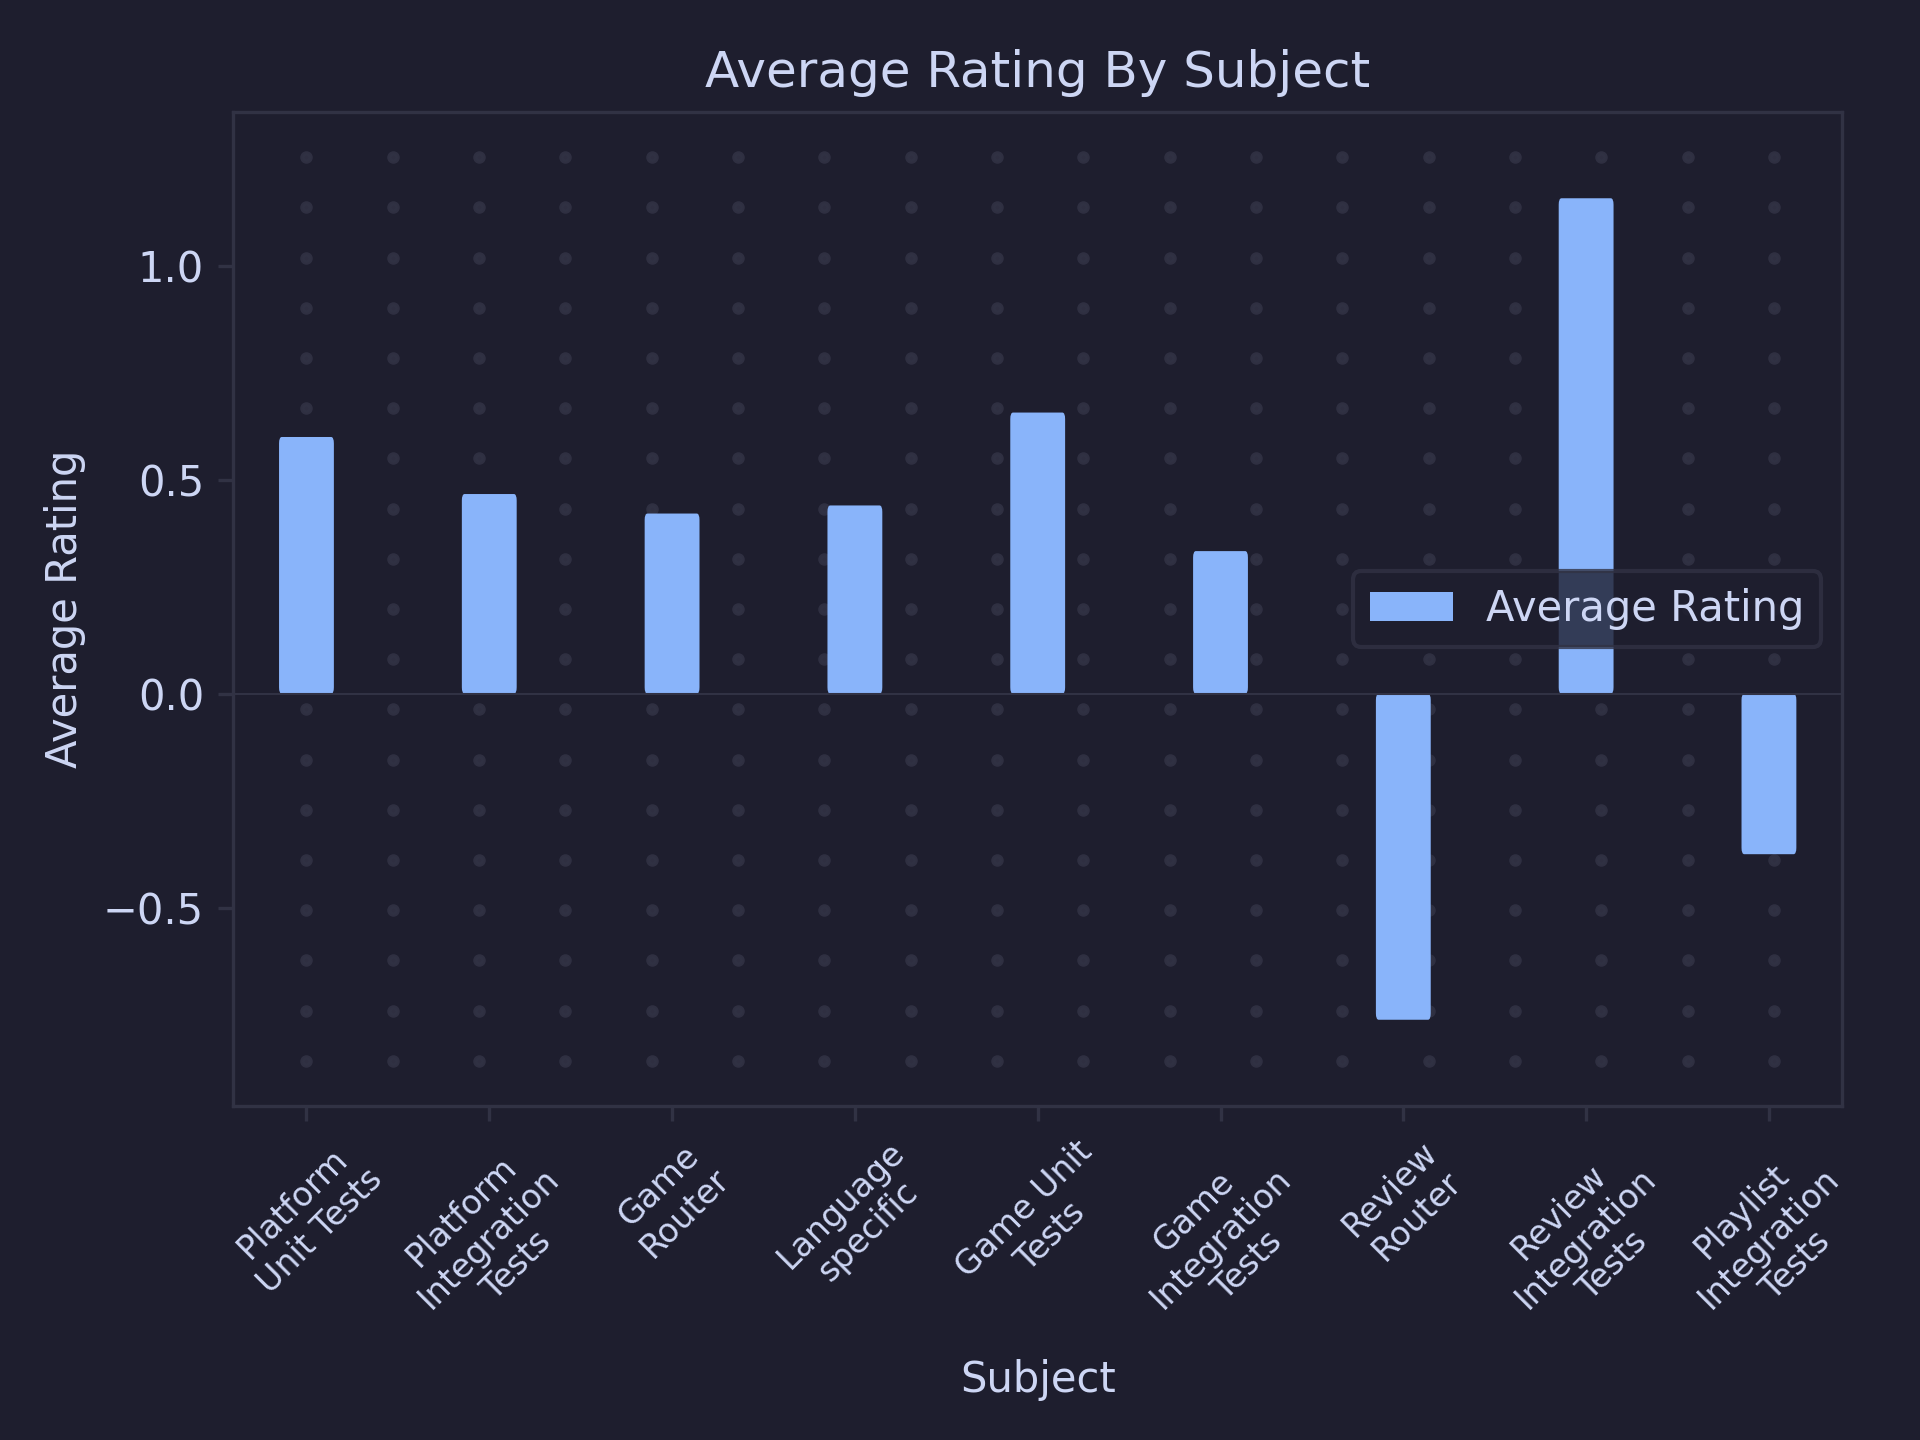
\includegraphics[width=0.85\textwidth]{subject_query_3.png}
      \caption{Μέσος όρος αξιολόγησης απαντήσεων για θέματα, \textit{μέρος
      3}}
    \end{center}
    \label{fig:SubjectQuery3}
  \end{figure}

  Από τα σχήματα \ref{fig:SubjectQuery1}, \ref{fig:SubjectQuery2} και
  \ref{fig:SubjectQuery3}, παρατηρείται ότι δεν υπάρχει κάποια
  συγκεκριμένη τάση στην αξιολόγηση των απαντήσεων ανά θέμα, με τα
  περίσσοτερα των θεμάτων να έχουν θετικό μέσο όρο. Αξιοσημείωτη η
  περίπτωση του θέματος της ανάπτυξης της λειτουργίας του προγραμματιστή
  του παιχνιδιού (\textlatin{Developer Router}), όπου στις πρώτες
  προτροπές, δεν δόθηκε στο μοντέλο κάποια κατεύθυνση, με αποτέλεσμα οι
  απαντήσεις που παρήχθηκαν να αξιολογηθούν αρνητικά, ενώ στις επόμενες
  προτροπές, οι απαντήσεις που παρήχθηκαν αξιολογήθηκαν κατά μέσο όρο ίσο
  με μηδέν (0), παρατηρώντας την μεγαλύτερη αύξηση στο μέσο όρο
  αξιολογήσεων από θέμα σε θέμα.

  Το θέμα \textlatin{Manual Intervention} αφορούσε τις περιπτώσεις που ο
  προγραμματιστής αναγκάστηκε να επενέβει, με σκοπό να αποφευχθούν
  συνεχόμενες αρνητικές αξιολογήσεις στο ίδιο θέμα μετά από μια σειρά
  λάθος απαντήσεων.

  \section{Συμπεράσματα}

  Ώντας μια καινοτόμος επιλογή τεχνολογικής στοίβας, η χρήση της
  \textlatin{Typescript}, σε συνδυασμό με το \textlatin{tRPC} και το
  \textlatin{Prisma}, αποτέλεσε μια πρόκληση για το μοντέλο του
  \textlatin{GitHub Copilot}. Η επιλογή αυτή έγινε με σκοπό την ορθότερη
  αξιολόγηση της ικανότητας του μοντέλου να ακολουθήσει την ταχεία εξέλιξη
  των τεχνολογιών και συγκεκριμένα στο οικοσύστημα της
  \textlatin{Javascript}, καθώς έχει συνεχείς προσθήκες και αλλαγές στον
  τρόπο που γράφεται ο κώδικας και επίσης αποτελεί τη βασική
  προγραμματιστκή γλώσσα του διαδικτύου.

  Εκ του αποτελέσματος των δοκιμών, η ιδανικότερη χρήση του μοντέλου του
  \textlatin{GitHub Copilot} φαίνεται είναι να ακολουθήσει τις επιλογές
  του προγραμματιστή για την ανάπτυξη του κώδικα, την αρχιτεκονική, τα
  πρότυπα σχεδίασης και τις βιβλιοθήκες που θα χρησιμοποιηθούν κατά την
  ανάπτυξη της εφαρμογής, όπως και αποδείχθηκε από τα αποτελέσματα στις
  περιπτώσεις που δόθηκε η ευκαιρία στο μοντέλο να λάβει αποφάσεις, καθώς
  οι περισσότερες αλλαγές που πραγματοποιήθηκαν από την πλευρά του
  προγραμματιστή ήταν σε μεγάλες εκτάσεις κώδικα και συγκεκριμένα στις
  περιπτώσεις των ελέγχων, όπου εκεί το μοντέλο έλαβε πρωτοβουλίες κατά τη
  σύνταξη των ελέγχων, οδηγώντας σε λάθη.
